\documentclass[12pt]{jreport}
\usepackage[dvipdfmx]{graphicx}
\usepackage{fancybox}
\usepackage{ascmac}
\usepackage{amsmath}
\usepackage{array,arydshln}
\usepackage{url}
\usepackage{comment}
\usepackage{amssymb}
\usepackage{multirow}
\usepackage{url}

\def\figurename{Figure}
\def\tablename{Table}
\def\bibname{参考文献}

\setlength{\topmargin}{-1.0cm}
\setlength{\oddsidemargin}{1.0cm}
\setlength{\evensidemargin}{1.0mm}
\setlength{\textwidth}{15cm}
\setlength{\textheight}{23cm}
\setcounter{topnumber}{5}%    ページ上部の図表は 5 個まで
\def\topfraction{1.00}%       ページの上 1.00 まで図表で占めて可
\setcounter{bottomnumber}{5}% ページ下部の図表は 5 個まで
\def\bottomfraction{1.00}%    ページの下 1.00 まで図表で占めて可
\setcounter{totalnumber}{10}% ページあたりの図表は 10 個まで
\def\textfraction{0.0}%      ページうち本文が占める割合の下限
\def\floatpagefraction{0.7}%  図表だけのページは少なくともこれだけを図表が占める

\newcommand{\IB}{$\bullet$}
\newcommand{\IC}{$\circ$}
\newcommand{\IS}{$\ast$}


\begin{document}%ドキュメントの始まり
\baselineskip=0.8cm%タイトルの行間隔
%\input{cover.tex}%外タイトル
 %!TEX root = ../main.tex

\newcommand{\hdate}[1]{\setcounter{page}{0}\begin{center}{\LARGE
#1\\}\vskip 10pt {\Huge 修士論文}\end{center}\vskip 40pt}


%題目が入ります
\newcommand{\htitle}[1]{
        \begin{center}
%                {\LARGE 題目}\\
                \vskip 16pt
                {\LARGE #1}\\
                \setlength{\unitlength}{1mm}
%               \vskip -20pt
%               \begin{picture}(120,10)(0,0)
%                       \put(0,0){\thicklines\line(1,0){120}}
%               \end{picture}
        \end{center}
        \vskip 40pt
}

\begin{titlepage}
\vspace*{2cm}
\hdate{2025年度}
\htitle{太陽光発電による電力グリッドに対する\\数理モデルを用いた運用最適化手法}

\hspace{8cm}
\begin{center}
\Large

神戸大学大学院システム情報学研究科\\
システム情報学専攻\\

\vskip 20pt
奥村~侑真\\
\vskip 50pt

\begin{tabular}{llll}
指導教員 & & {\Large 玉置　久} & 教授 \\ \cline{1-4}
審査教員 & 主査 & {\Large 玉置　久} & 教授 \\ \cline{1-4}
         & 副査 & {\Large 浦久保　孝光} & 教授 \\ \cline{2-4}
\end{tabular}

\vskip 40pt

2026年2月5日
\end{center}
\end{titlepage}%内タイトル

%% 著者近影

\vspace*{15cm}
\begin{flushleft}
\hspace*{-9mm}
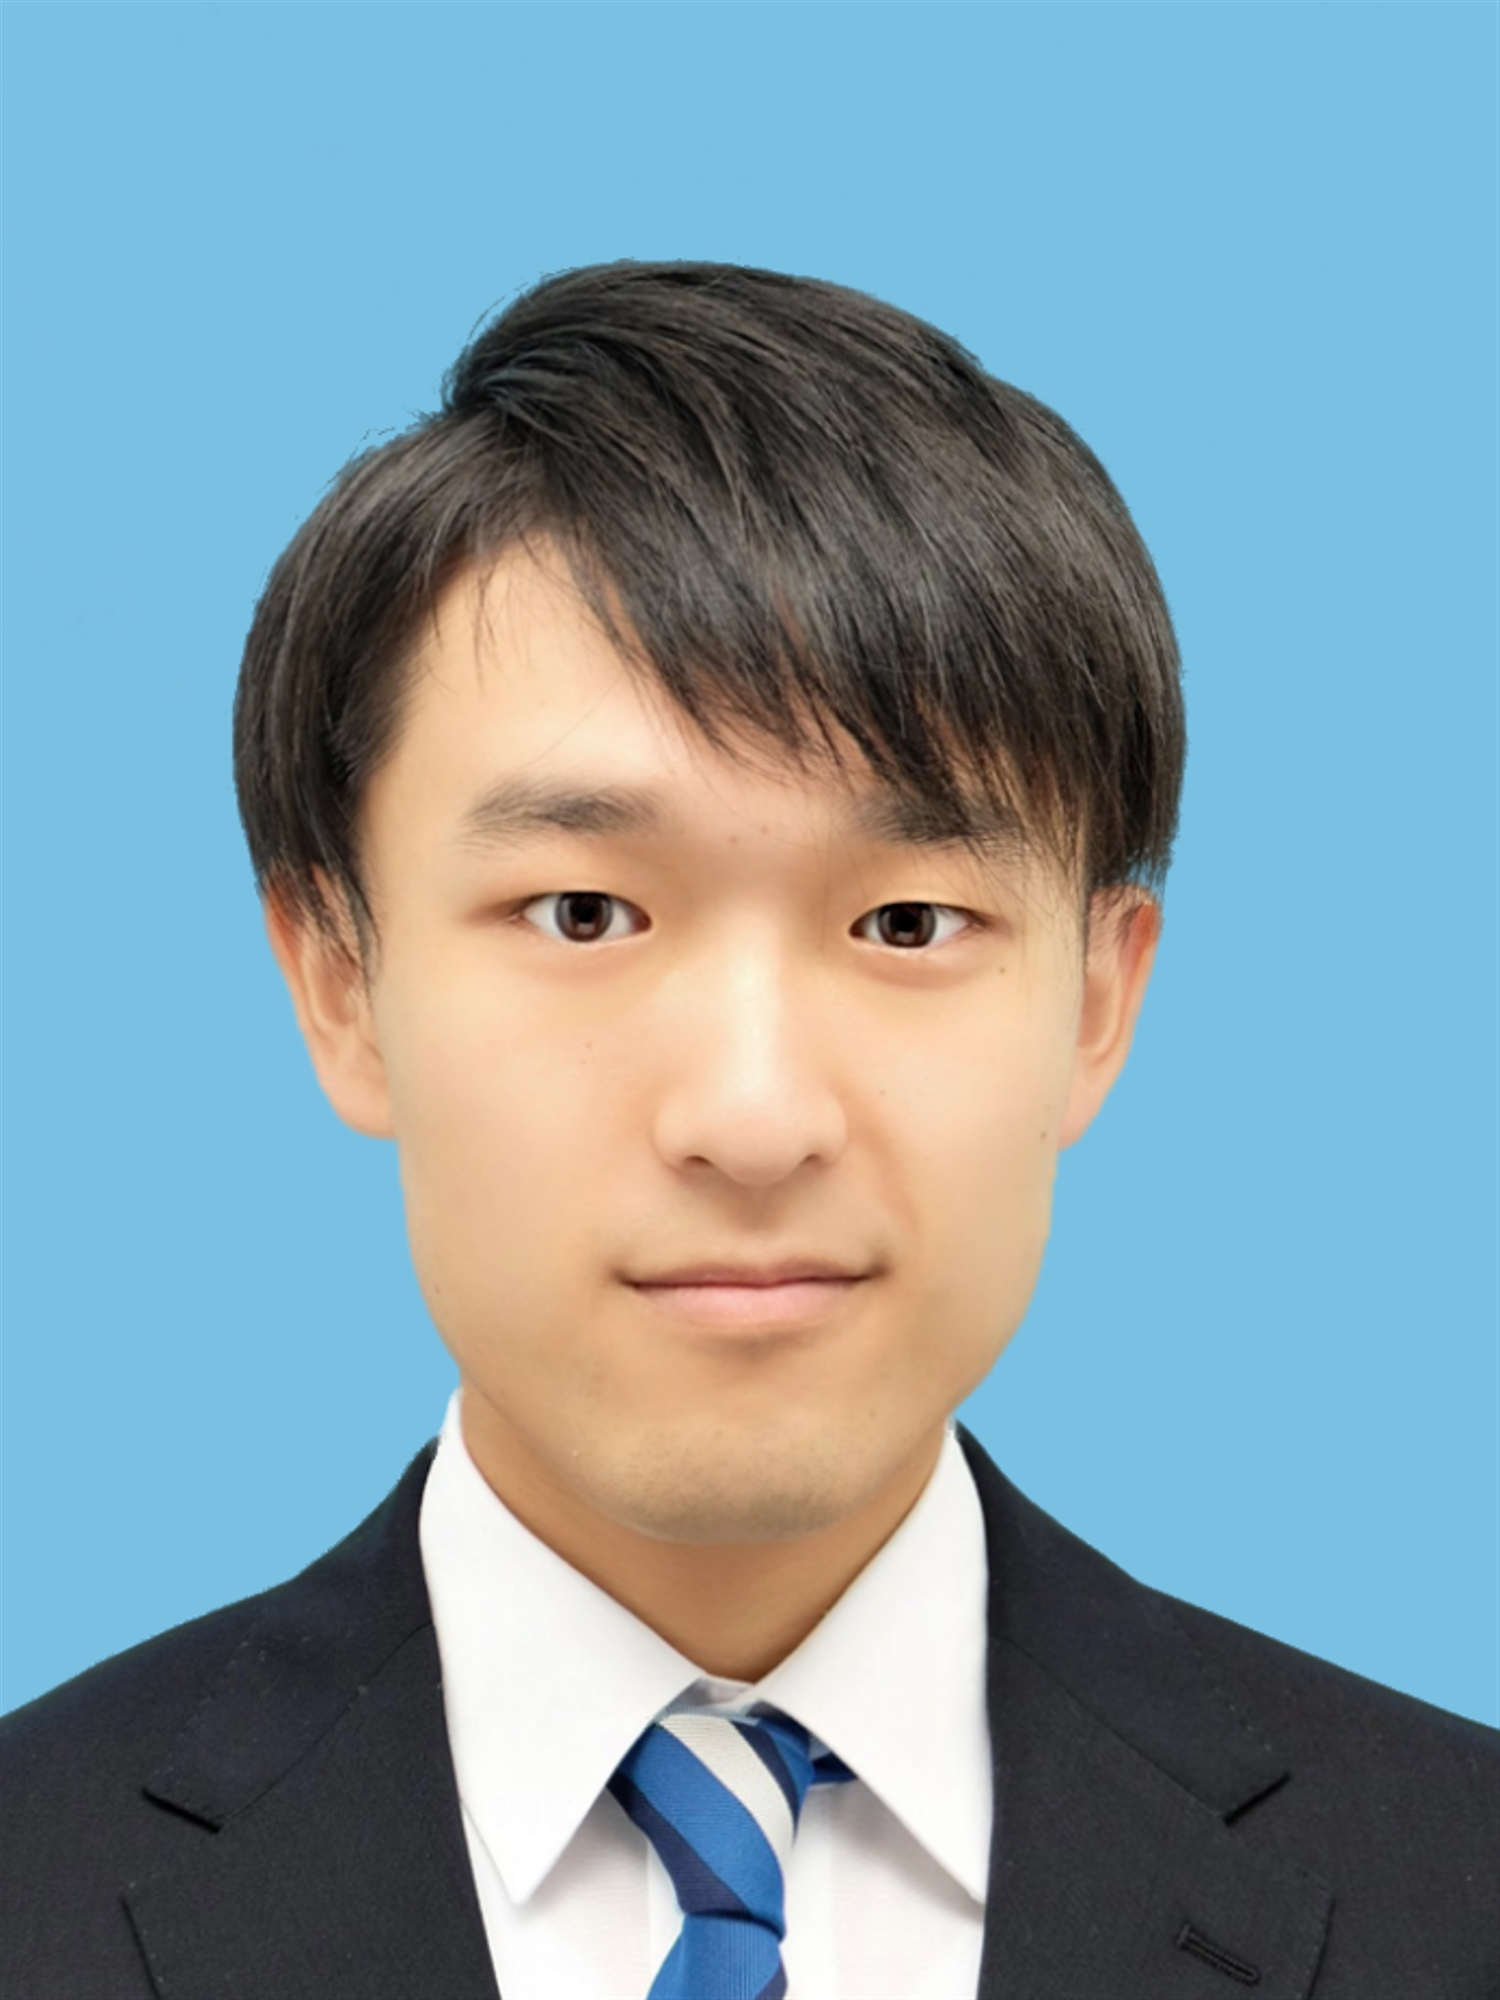
\includegraphics[height=6cm]{fig/okumura.jpg}
\end{flushleft}
\vspace*{-4mm}
\hspace*{-8mm}
Copyright \copyright \, 2026, Yuma Okumura
\newpage


\baselineskip=0.75cm%要旨の行間隔

% 英文要旨
\thispagestyle{empty} %英文要旨ページ番号なし
%!TEX root = ../main.tex
\begin{center}

{\LARGE \bf Operational Optimization Methods Using Mathematical Models for a Power Grid with Photovoltaic Generation}
\\[0.7cm] 
{\Large YUMA OKUMURA}
\\[1.0cm]
{\LARGE \bf ABSTRACT}
\end{center}

In recent years, initiatives such as ``Carbon Neutrality by 2050'' and the ``GX2040 Vision'' have been promoted to address global warming, accelerating the deployment of renewable energy. While photovoltaics are anticipated to play a substantial role as distributed power sources, their fluctuations of weather-dependent output disrupt the grid's supply-demand balance. As a result, effective power management using battery storage systems has become an increasingly important issue. In particular, with the spread of market-linked electricity pricing schemes, it has become crucial to formulate economically efficient charging and discharging schedules that respond to market supply-demand conditions.
This study proposes an optimal operational method aimed at reducing costs and improving efficiency in a power grid system---comprising photovoltaic facilities, storage batteries, and self-consignment destinations---modeled on a factory located in Kochi Prefecture. Specifically, two mathematical models---a linear programming model and a dynamic programming model---are constructed to compare and verify their computational characteristics and practical applicability. The linear programming model derives exact solutions by setting multiple objective functions, such as minimizing electricity purchasing costs and minimizing net expenditure while accounting for revenue from surplus power sales. In contrast, the dynamic programming model discretizes battery capacity and is formulated through the Bellman equation based on the principle of optimality.
Experiments using real data from July 2025 show that although both models yield reasonable operational plans, distinct differences appear in their computational characteristics. The linear programming model is more sensitive to constraints, whereas the dynamic programming model demonstrates stable scalability, with computation time increasing linearly with the length of the planning period. In conclusion, this study establishes guidelines for model selections in the real environments: the linear programming model is effective for short-term planning and high-precision operations, while the dynamic programming model is preferable when long-term planning and predictable computation times are prioritized.




% 和文要旨

\thispagestyle{empty} %和文要旨ページ番号なし
%!TEX root = ../main.tex
\begin{titlepage}

\begin{center}
{\LARGE \bf 太陽光発電による電力グリッドに対する\\数理モデルを用いた運用最適化手法}
\\[0.7cm]
{\Large 奥村~侑真}
\\[1.0cm]
{\LARGE \bf 要\vspace{36pt}   旨\\}
\end{center}

近年，地球温暖化対策として「2050年カーボンニュートラル」や「GX2040ビジョン」が掲げられ，再生可能エネルギーの導入が加速している．その中でも太陽光発電は分散型電源として期待されているが，気象条件による出力変動が電力系統の需給バランスに影響を与えるため，蓄電池を活用した電力運用が急務となっている．
特に，市場連動型料金プランの普及に伴い，電力市場の需給に応じた経済的な充放電計画を実運用における時間的制約条件下で策定することが肝要である．本研究では，徳島県内のある工場をモデルとした，太陽光発電設備，蓄電池，および自己託送先を含む電力グリッドシステムを対象とし，その運用コスト削減と効率化を目的とした最適な運用手法を提案する．具体的には，線形計画モデルと動的計画モデルの2つの数理モデルを構築し，それぞれの計算特性や実用性を比較・検証した．線形計画モデルでは，買電コストの最小化や余剰電力の売電益を考慮した正味支出の最小化など複数の目的関数を設定し，厳密解の導出を行った．一方，動的計画モデルでは，蓄電池容量を離散化し，逆方向の最適性の原理に基づくBellman方程式を用いて定式化した．
2025年7月の陽光発電および需要電力の実データを用いた実験の結果，両モデルとも合理的な運用計画を導出したが，計算特性には差異が確認された．線形計画モデルは制約条件の影響を受けやすい一方，動的計画モデルは計画期間に対し計算時間が線形に増加する安定したスケーラビリティを示した．結論として，短期間の高精度な運用には線形計画モデル，長期間の計画や計算時間の予測性を重視する場合には動的計画モデルが有効であるという，実環境における選定指針を明らかにした．
\end{titlepage}



% 目次
%\baselineskip=0.7cm%%%%目次の間隔狭い時ON
\baselineskip=0.9cm%%%%%目次の行間隔
\pagenumbering{roman}%%%目次のページ番号roman
\tableofcontents%%%%%%%%目次
\newpage%%%%%%%%%%%%%%%%改ページ

% 本文
\baselineskip=0.7cm%%%%%本文の行間隔
\pagenumbering{arabic}%%本文のページ番号arabic
\setcounter{page}{1}%%%%本文のページ1から開始

% 序論
%!TEX root = ../main.tex

\chapter{序論}
近年，地球温暖化対策としての温室効果ガス排出削減は世界的に課題となっている．日本政府は「2050年カーボンニュートラル」を掲げ，2025年2月にはエネルギー安定供給，経済成長，脱炭素の同時実現を目指す「GX2040ビジョン」を閣議決定した． 日本のエネルギー自給率は2023年度時点で15.3％とG7諸国で最低水準にあり，ロシアによるウクライナ侵略や中東情勢の緊迫化に伴う経済安全保障上のリスクが顕在化している．一次エネルギー供給の8割以上を海外からの輸入化石燃料に依存する現状において，国産の脱炭素エネルギー源である再生可能エネルギーの導入加速が急務となっている\cite{a1}．

再生可能エネルギーの中でも，太陽光発電は比較的リードタイムが短く，工場や公共施設等の屋根を活用した分散型電源として期待されている．しかし，太陽光発電は気象条件に依存して出力が変動するため，大量導入は電力系統の需給バランスを不安定化させる要因となる． このため，地域内での出力制御が増加しており，系統への負荷を抑えつつ再エネを有効活用するための「自家消費」や「需給近接型」の運用が重要視されている．特に，市場連動型の電力料金プランの普及に伴い，発電事業者自らが電力市場の需給に応じた供給計画を策定し，蓄電池等の調整力を活用して運用を高度化させることが求められている\cite{a1}．

電力グリッドの最適化に関しては，多様な数理的アプローチが提案されている． 岩瀬（2017）は，電気と熱の融通を考慮した分散型エネルギーグリッドの数理計画モデルを構築し，一次エネルギー消費量とCO2排出量の削減効果を定量的に評価した\cite{a3}．秋山（2013）は，東日本大震災後の電力供給の脆弱性を背景に，直流マイクログリッドにおける電力利用効率向上を目指し，据置型だけでなく移動型バッテリーを併用した混合整数計画モデルを提案した\cite{a4}．また，三浦（2015）は，兵庫県南あわじ市の沼島をモデルとした実証研究を補完するため，住民の電力消費行動を模擬するエージェントモデルとシステムモデルを統合したシミュレーションを行い，災害時の自立性やCO2削減効果を検証した\cite{a5}． これらの研究は，数理計画やシミュレーションを用いてシステムの有効性を示している．しかし，需要予測や市場単価が刻々と変動する実運用の現場において，限られた計算時間内でいかに迅速かつ確実に最適解を導出するかという，具体的な実装・適用フェーズにおける実用的な検討については，依然としてさらなる検討の余地がある．

本研究では，先行研究の知見を踏まえつつ，より実務的な運用手法の確立を目指す．具体的には，徳島県内の工場をモデルとした電力グリッドシステムを対象とし，市場連動型料金体系や自己託送制度を考慮した蓄電池運用の最適化モデルを構築する． 本研究の独自性は，線形計画法と動的計画法の2つの手法を同一モデルに適用し，その計算パフォーマンスや実用性を比較・検証する点にある．これにより，工場のエネルギーマネジメントにおける最適な数理的手法の選定指針を提示する．

本論文の構成は以下の通りである． まず第2章では，本研究の対象となる太陽光発電設備，蓄電池，および自己託送先を含む電力グリッドシステムの構成と，運用において満たすべき諸条件について述べる． 第3章では，連続値を扱うことで高精度な最適化が可能な線形計画モデルの定式化について，目的関数や制約条件の詳細を説明する． 第4章では，蓄電池の状態を離散化し，長期間の計画に対して効率的な計算が期待できる動的計画モデルの構築と，最適性の原理に基づくBellman方程式の適用について述べる． 第5章では，実データを用いた計算機実験の結果を示し，線形計画法と動的計画法の双方の観点から，計画期間や離散化数が計算時間に与える影響を比較・検討する． 
最後に第6章では，本研究で得られた知見を総括し，今後の課題と展望について述べる．

% 
%!TEX root = ../main.tex

\chapter{太陽光発電による電力グリッドシステム}
\section{電力グリッドの概要}
電力グリッド(電力系統，Electrical grid)とは，発電した電力を電力を必要とする設備に供給するために，発電・変電・送電・配電・充放電の各工程を統合したシステムである．

\section{本研究で扱う対象}
本研究では高知県の某工場を対象とする．本研究の対象は以下の要素で構成されている．
\begin{itemize}
	\item 電力の導線
	\item 太陽光発電設備\\
	工場屋上に設置された発電設備．
	\item 電力消費機器\\
	空調照明，および製造用機械など，電力を消費する設備群．本研究の対象では設備群が3つ存在する．
	\item 蓄電池\\
	電力量の需給調整や非常用電源として機能する設備．
	\item 電力変換装置\\
	パワーコンディショナや変圧器などの，電圧を変換したり，交流から直流，あるいはその逆に変換する設備.
	\item 商用電力系統\\
	卸売電力取引所や電力会社から電力を購入・受電したり，電力を売電するために接続されている外部系統． 
	電力を購入するにあたり，単位電力量あたりの料金単価は市場価格に応じて変動する． 
	また，連続する30分間の平均使用電力を需要電力とし，
	その月の最大需要電力と過去11ヶ月の最大需要電力のうち，大きい方の値を基準に契約電力が決定され，契約電力に応じて基本料金が課される．\cite{m}
	\item 自己託送先\\
	自社で発電した余剰電力を，外部のネットワークを介して送電する設備群．
	\item 余剰電力の破棄先\\
	発電した電力が需要や蓄電容量，および売電可能量を超過した場合に，
	余剰分を破棄するための仮想的な領域．
	数理モデル上では電力の破棄として扱われるが，物理的にはパワーコンディショナの出力制御機能による発電量の抑制に相当する．	
\end{itemize}
	
本研究における電力運用の大きな特徴は，構成要素に太陽光発電設備と蓄電システムが含まれている点，
および商用電力系統からの買電単価が市場に応じて変動する点にある．%また，余剰電力を自己託送する要求が存在する点も特徴的である．
したがって，将来の予測発電量や予測消費電力量，予測料金単価%，および自己託送先の需要予測値
を踏まえつつ，
いかなるタイミングでどの程度の電力を蓄電池に充放電させるかを決定することが肝要となる．本研究で扱う対象を図\ref{fig:tecseed}に示す．
\begin{figure}[h]
	\centering
 	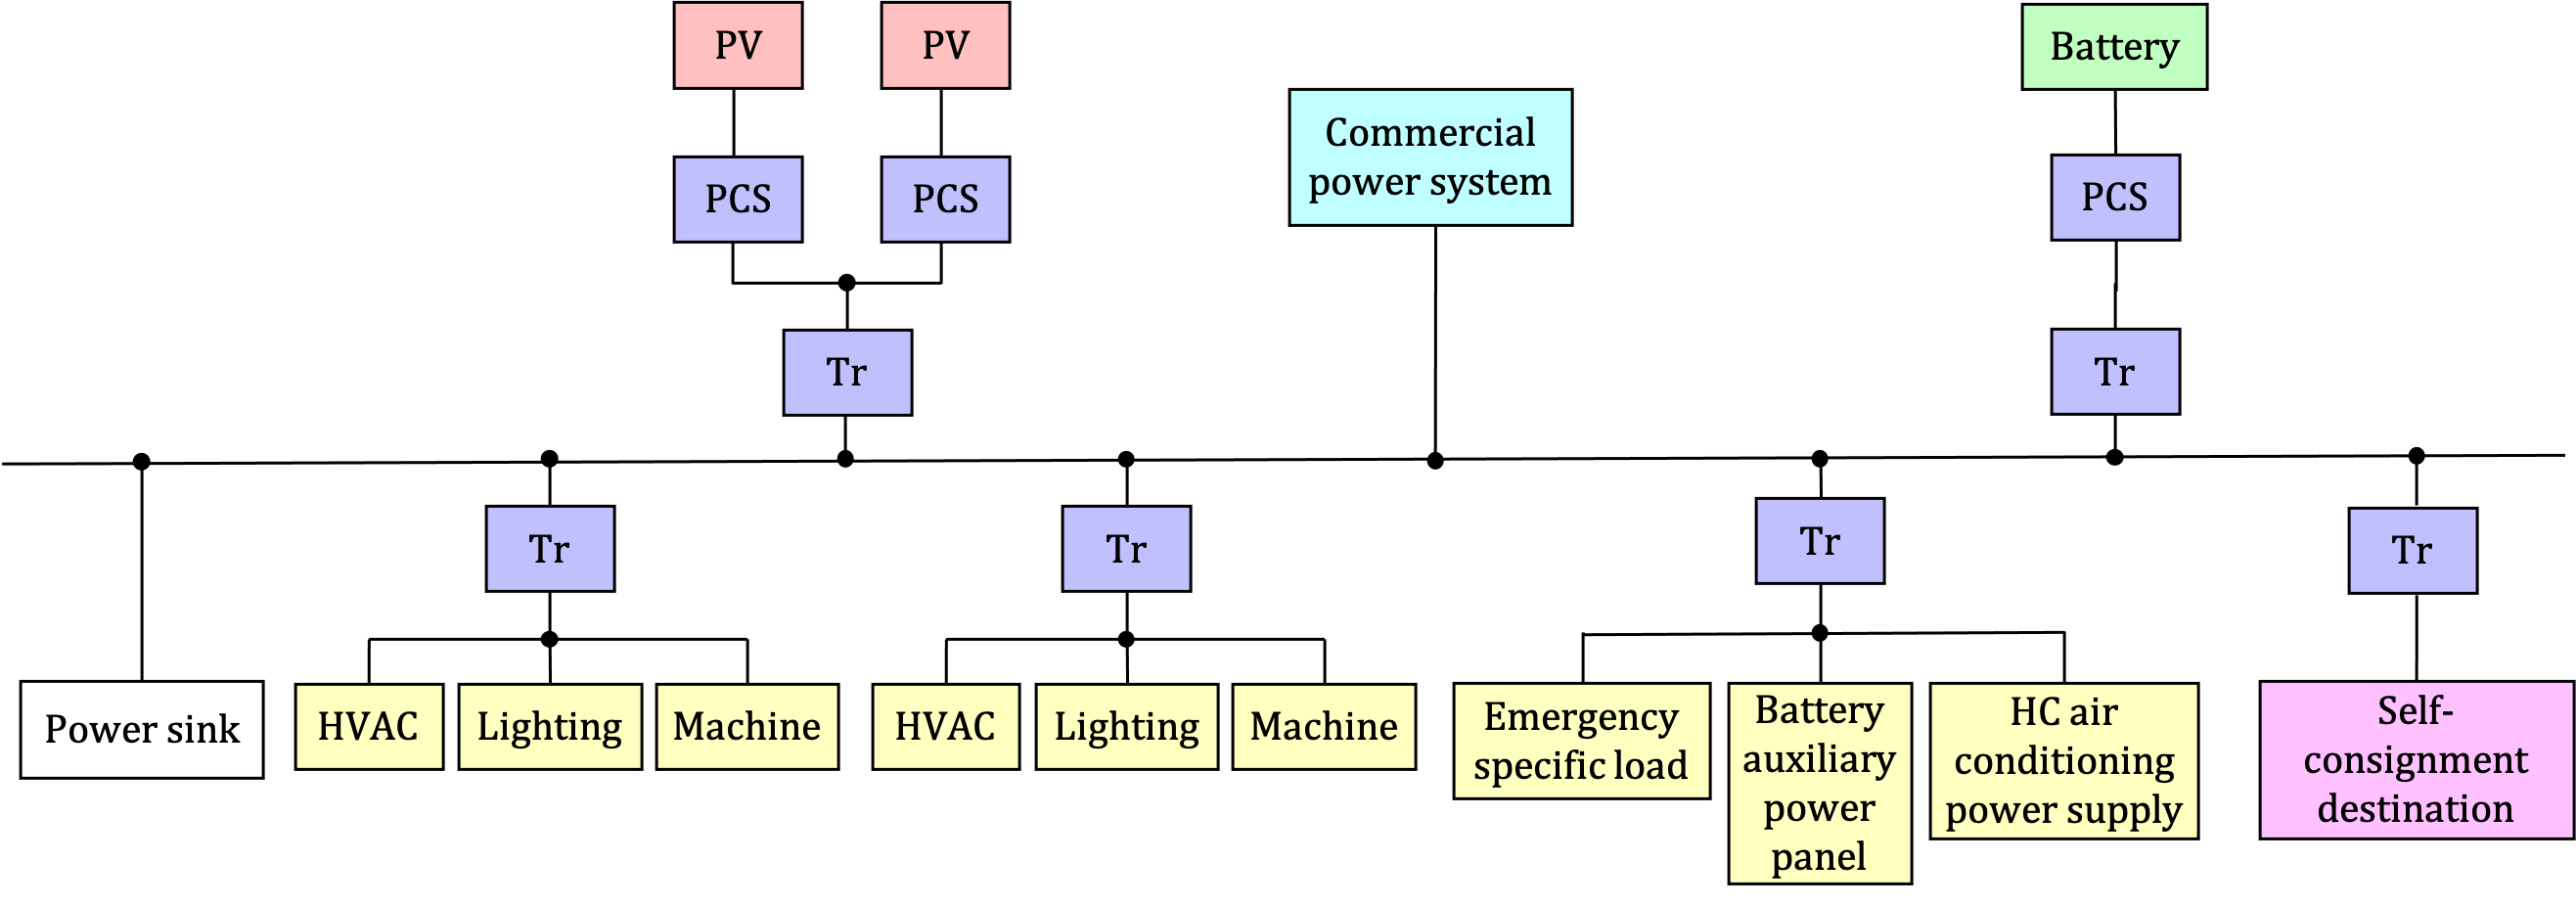
\includegraphics[width=215mm ,angle=270]{../figure/food_techno_eng.png}
 	\caption{Architecture of target system(PV: Photovoltaic, PCS: Power Conditioning System, Tr: Transformer)}
 	\label{fig:tecseed}
\end{figure}

\section{本研究で扱う対象が満たすべき事項}\label{sec:object}
本研究で扱う電力グリッドをモデル化するにあたり，考慮すべき事項を，モデル構築の基礎となる前提条件，設備や運用ルールに基づく制約条件，および最適化によって達成を目指す運用目的上の条件の3つに分類して定義する．

\subsection{モデル化における前提条件}
本研究の数理モデルにおいて，物理的な整合性を保つために導入する仮定である．
\begin{itemize}
	\item 導線\\
	導線の各接続点において，流入する電力と流出する電力の総和が等しいものとする．
	\item 電力変換装置 \\
	パワーコンディショナや変圧器などを介して電力を変換・送電する際，一定の変換効率に応じた電力損失が発生するものとする．
\end{itemize}

\subsection{システムおよび運用上の制約条件}\label{sec:object_seiyaku}
各設備の仕様および，電力契約や制度上のルールとして遵守しなければならない事項である．
\begin{itemize}
	\item 蓄電池
	\begin{itemize}
		\item 蓄電池の残量は常に定められた範囲内を外れないこと．
		\item 単位時間あたりの充放電電力は，最大出力を超過しないこと．
	\end{itemize}
	\item 商用電力系統 \\
	任意の連続する30分間の区間について，商用電力系統からの総買電力を一定量以下に制限すること．
	\item 自己託送先 \\
	自己託送先の需要電力量を上回る送電を行わないこと．
\end{itemize}

\subsection{運用目的上の条件}
上記の制約条件を満たした実行可能領域の中で，最適化によって最大化・最小化を目指す評価指標である．
\begin{itemize}
	\item 商用電力系統 \\
	期間内の商用電力からの買電コストを最小化すること．
	\item 自己託送先 \\
	可能な限り多くの余剰電力を自己託送に回すこと．
\end{itemize}



%モデル
%!TEX root = ../main.tex

\chapter{ 線形計画モデル}
問題の対象となるモデルを線形な等式・不等式制約の集合として表現できる場合，
線形計画法を適用することが合理的である．線形計画法を用いる主な利点として，
変数を連続値として扱えるため，離散化誤差が生じない点が挙げられる．本章では，まず線形計画法を用いたモデル化について述べる．

\section{本研究での時間の扱い}
計画対象となる期間の先頭の時刻を時刻0とし，当該期間を等間隔に$K$個の区間に分割する．
分割された各々の区間の区間幅を$\Delta t$とし，これ以降この区間のことを以降「期」とよぶ．
特に，時刻$(k-1)\Delta t$から時刻$k\Delta t$までの区間のことを「$k$期」と定義する．

以降，各々の変数について期の情報を伴う場合は，その変数に$1,\dots,K$のインデックスを付す．その下で，
太陽光発電電力量や電力需要量など，期間で定義される変数$E_k(k=1,\dots ,K)$は$k$期における総量として定義し，
蓄電池の残量など，時点の状態で定義される変数$S_k(k=1, \dots , K)$については各々の期の末尾で定義する．
なお，例外的に計画期間における初期状態は$S_0$のように表す．時間の扱いについてのイメージを図\ref{fig:time_dig_lp}に示す．

\begin{figure}[h]
	\centering
 	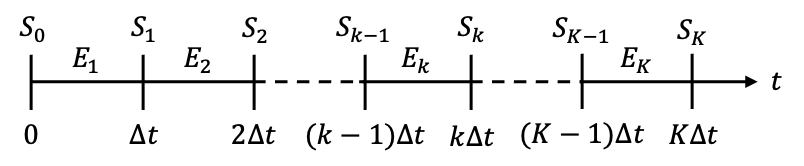
\includegraphics[width=155mm]{../figure/time_dig.png}
 	\caption{Period and measured time}
 	\label{fig:time_dig_lp}
\end{figure}

\section{モデルの要素}
\ref{sec:object}節で示したモデルの要素(\IS を付して記す)と，これらの要素に付随する定数(\IB を付して記す)，変数(\IC を付して表す)を列挙する．
モデル中の定数・変数と電力グリッドとの関係を図\ref{fig:variables_lp}に示す．
赤色の文字は決定変数，青色の文字は従属変数，緑色の文字は外生変数である．
なお，定数・変数の傍らに灰色で付記された文字は，その定数・変数が後述する当該のケースを採用した場合にのみ現れることを表している．

\begin{itemize}
 	\item[\IS] 太陽光発電設備G
		\begin{itemize}
		 	\item[\IB] 太陽光発電電力量(変換前) $g^{\rm P1}_{k}$
  			\item[\IC] 太陽光発電電力量(変換後) $g^{\rm P2}_{k}$
		\end{itemize}	
	 \item[\IS] 電力消費機器D$^{\rm A}$
	 	\begin{itemize}
		 	\item[\IC] 電力需要量A (変換前) $d^{\rm A1}_{k}$
 			\item[\IB] 電力需要量A (変換後) $d^{\rm A2}_{k}$
		\end{itemize}
 	\item[\IS] 電力消費機器D$^{\rm B}$
	 	\begin{itemize}
		 	\item[\IC] 電力需要量B (変換前) $d^{\rm B1}_{k}$
 			\item[\IB] 電力需要量B (変換後) $d^{\rm B2}_{k}$
		\end{itemize}	
 	\item[\IS] 電力消費機器D$^{\rm C}$
	 	\begin{itemize}
		 	\item[\IC] 電力需要量C (変換前) $d^{\rm C1}_{k}$
 			\item[\IB] 電力需要量C (変換後) $d^{\rm C2}_{k}$
		\end{itemize}
 	\item[\IS] 電力消費機器（自己託送先）D$^{\rm D}$
 	\begin{itemize}
   		\item[\IB] 自己託送先が必要とする電力 $d^{\rm D}$
   		\item[\IB] 自己託送先へ託送することのインセンティブ係数 $p^{\rm D}$   
		\item[\IC] 自己託送先への託送量 (変換前) $d^{\rm D1}_{k}$
 		\item[\IC] 自己託送先への託送量(変換後) $d^{\rm D2}_{k}$
  	\end{itemize} 
 	\item[\IS] 蓄電池B$^{\rm F}$
  		\begin{itemize}
   			\item[\IB] 蓄電池の最大容量 $\overline{b}^{\rm F}$
			\item[\IB] 蓄電池の初期残量 $b^{\rm F}_{0}$
		  	\item[\IC] 蓄電池の(期末の)残量 $b^{\rm F}_{k}$
  			\item[\IC] 蓄電池の充電量(変換前) $x^{\rm FC1}_{k}$
  			\item[\IC] 蓄電池の充電量(変換後) $x^{\rm FC2}_{k}$
			\item[\IC] 蓄電池の放電量(変換前) $x^{\rm FD1}_{k}$
			\item[\IC] 蓄電池の放電量(変換後) $x^{\rm FD2}_{k}$
			 \item[\IB] 単位時間あたりの最大充電電量 $a^{\rm FC}$
  			\item[\IB] 単位時間あたりの最大放電量 $a^{\rm FD}$
  		\end{itemize}
 	\item[\IS] 電力変換装置(太陽光) E$^{\rm P}$
  		\begin{itemize}
   			\item[\IB] 変換効率 $\alpha^{\rm P}$
  		\end{itemize}
 	\item[\IS] 電力変換装置(商用電力系統) E$^{\rm S}$
 	\item[\IS] 電力変換器(消費機器A) E$^{\rm DA}$
  		\begin{itemize}
   			\item[\IB] 変換効率 $\alpha^{\rm DA}$
 		\end{itemize}
 	\item[\IS] 電力変換器(消費機器B) E$^{\rm DB}$
  		\begin{itemize}
  	 		\item[\IB] 変換効率 $\alpha^{\rm DB}$
 	 	\end{itemize}
 	\item[\IS] 電力変換器(消費機器C) E$^{\rm DC}$
	  	\begin{itemize}
	   		\item[\IB] 変換効率 $\alpha^{\rm DC}$
	 	 \end{itemize}
  	\item[\IS] 電力変換器(消費機器D) E$^{\rm DD}$
  	\begin{itemize}
   		\item[\IB] 変換効率 $\alpha^{\rm DD}$
  	\end{itemize} 
	
 	%\item[\IS] 蓄電池の自己放電に相当する仮想的な変換器 Z$^{ -1}$
  		%\begin{itemize}
   			%\item[\IB] 期$k$の先頭から期$k$の末尾にかけての自己放電効率$\alpha^{\rm FT}$
  		%\end{itemize}
 	\item[\IS] 電力変換器(蓄電池)E$^{\rm BF}$
  		\begin{itemize}
   			\item[\IB] 充電効率 $\alpha^{\rm FC}$
   			\item[\IB] 放電効率 $\alpha^{\rm FD}$
			\item[\IB] 自己放電効率 $\alpha^{\rm FT}$
  		\end{itemize}
 	\item[\IS] 商用電力系統S
   		\begin{itemize}
		  	\item[\IC] 系統買電力量$s^{\rm BY}_{k}$
			\item[\IB] 系統最大買電力量 $a^{\rm BY}$
   			\item[\IB] 系統電力量料金単価 $p^{\rm BY}_{k}$
   			\item[\IB] 系統基本料金単価 $p^{\rm BYMax}$
   			\item[\IB] 系統売電単価 $p^{\rm SL}_{k}$
			\item[\IC] 系統売電力量$s^{\rm BY}_{k}$
   			%\item[\IB] 単位時間あたりの最大系統売電量 $a^{\rm SL}_{k}$
  		\end{itemize}
 	\item[\IS] 余剰電力の破棄先O
	\begin{itemize}
	  	\item[\IC] 無駄電力量$w_{k}$
	\end{itemize}
\end{itemize}

\begin{figure}[h]
 \centering
 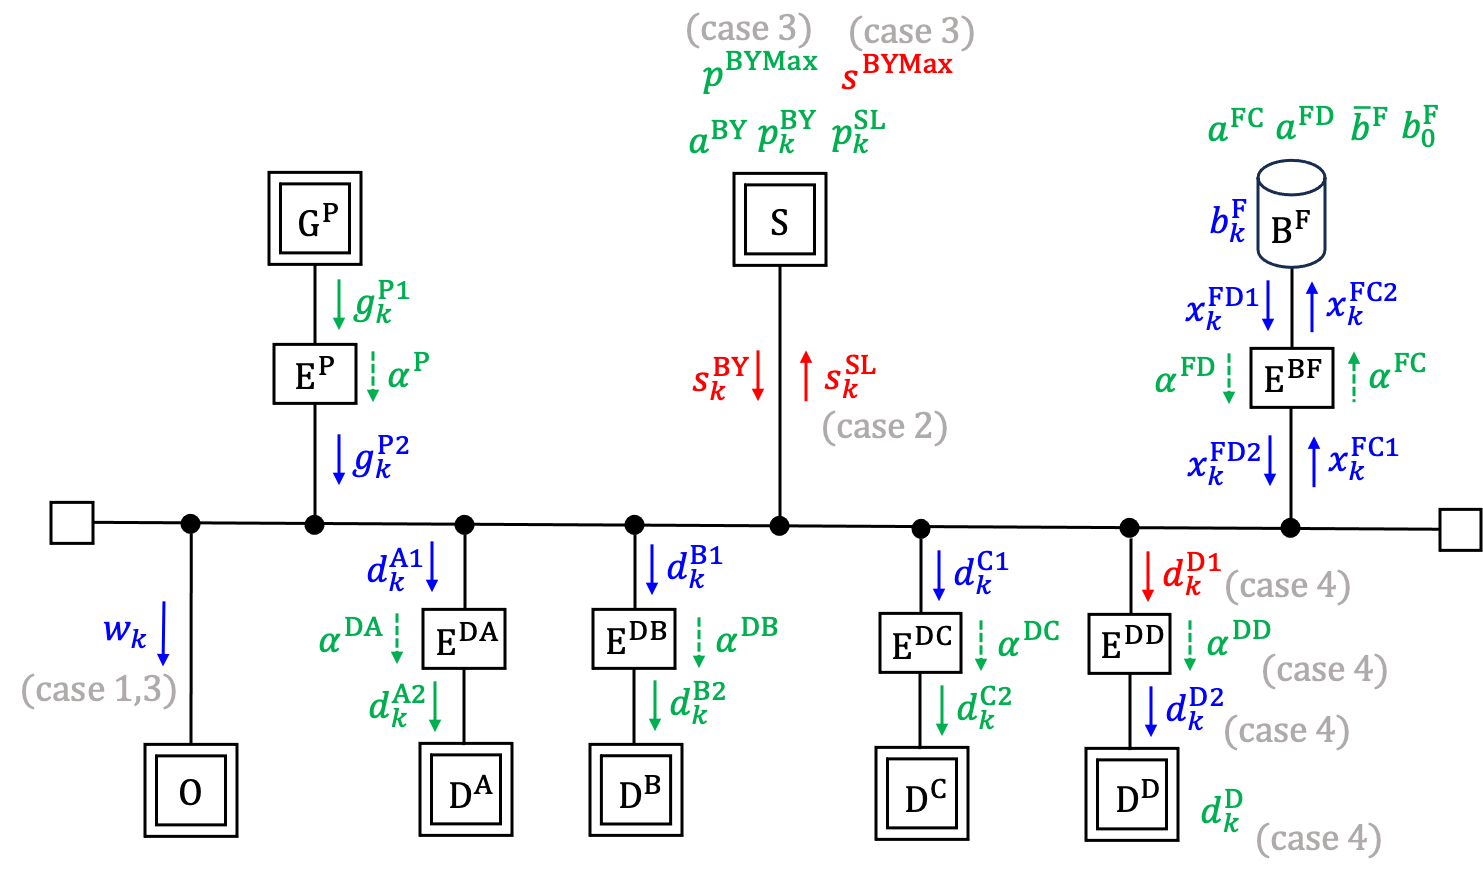
\includegraphics[width=140mm]{../figure/variables_lp.png}
 \caption{Configuration diagram of the target system(Linear Programming)}
 \label{fig:variables_lp}
\end{figure}

\section{目的関数}
最適化の目的は経済性の追求や環境価値の最大化など多岐にわたる．
ゆえに目的関数の定式化の方法は必ずしも一意に定まらない．
本研究では，対象となる工場の運用方針を考慮し以下の4つのケースを想定する．

買電コストを最小化するケース(以降「ケース1」とよぶ．)：
\begin{equation}
    \text{Minimize} \quad  \sum_{k=1}^{K}  ( p_k^{\rm{BY} } s_k^{\rm{BY}}  )．
 \label{eq:minimize_lp_1}
\end{equation}

余剰電力の売電を考慮し，金銭の正味の支出を最小化するケース(以降「ケース2」とよぶ．)：
\begin{equation}
    \text{Minimize} \quad  \sum_{k=1}^{K}  ( p_k^{\rm{BY} } s_k^{\rm{BY}} - p_k^{\rm{SL} } s_k^{\rm{SL}}  )．
 \label{eq:minimize_lp_2}
\end{equation}

基本料金を考慮し買電コストを最小化するケース（以降「ケース3」とよぶ．）：
 \begin{equation}
 	 \text{Minimize} \quad \sum_{k=1}^{K} ( p_k^{\rm{BY} } s_k^{\rm{BY}} + p^{\rm{BYMax} } s^{\rm{BYMax}} )．
 	 \label{eq:minimize_lp_3} 
\end{equation} 
なお，基本料金は契約電力に比例して決定される．実運用における契約電力は，当月を含む過去1年間の各月における最大需要電力
（30分間ごとの平均使用電力の最大値）のうち最も大きい値に基づいて決定されるが，
本研究では$K$期分における運用のみを評価対象とするため，
当該期間内における最大需要電力がそのまま契約電力を決定するものと仮定する．

支出を抑制しつつ，余剰電力の自己託送量をなるべく大きくするケース(以降「ケース4」とよぶ．)：
\begin{equation}
    \text{Minimize} \quad  \sum_{k=1}^{K}  ( p_k^{\rm{BY} } s_k^{\rm{BY}} - p^{\rm{D} } s_k^{\rm{D}}  )．
 \label{eq:minimize_lp_4}
\end{equation}


\section{制約条件}
\ref{sec:object_seiyaku}節で述べた事項を制約条件に書きかえたものを以下に列挙する．
ただし，特に断り書きがない場合，目的関数が(\ref{eq:minimize_lp_1})式〜(\ref{eq:minimize_lp_4})式のどのケースで表される場合について
も共通する制約条件である．また全ての変数は非負である．

\begin{itemize}
	\item 動線\\
		流入する電力と流出する電力の総和が等しいものとする(ケース1，ケース3の場合)
		\begin{equation}
			g^{\rm P2}_{k} + s^{\rm BY}_{k} 
 			- x^{\rm FC1}_{k} + x^{\rm FD2}_{k} 
 			- d^{\rm A1}_{k} - d^{\rm B1}_{k} - d^{\rm C1}_{k} - w_{k}= 0，
		 \quad
 		k=1,\dots,K
		~~
		\label{eq:line1}
		\end{equation}
		流入する電力と流出する電力の総和が等しいものとする(ケース2の場合)
		\begin{equation}
			g^{\rm P2}_{k} + s^{\rm BY}_{k} - s^{\rm SL}_{k}
 			- x^{\rm FC1}_{k} + x^{\rm FD2}_{k} 
 			- d^{\rm A1}_{k} - d^{\rm B1}_{k} - d^{\rm C1}_{k}  = 0，
		 \quad
 		k=1,\dots,K
		~~
		\label{eq:line23}
		\end{equation}
		流入する電力と流出する電力の総和が等しいものとする(ケース4の場合)
		\begin{equation}
			g^{\rm P2}_{k} + s^{\rm BY}_{k}
 			- x^{\rm FC1}_{k} + x^{\rm FD2}_{k} 
 			- d^{\rm A1}_{k} - d^{\rm B1}_{k} - d^{\rm C1}_{k}  = 0，
		 \quad
 		k=1,\dots,K
		~~
		\label{eq:line4}
		\end{equation}
	\item 蓄電池\\
		蓄電池の残量の推移についての関係式
		\begin{equation}
 			b_k^{\rm F} = \alpha^{\rm FT}b_{k-1}^{\rm F} + x_{k}^{\rm FC2} - x_{k}^{\rm FD1}
 			\quad
 			k=1,\ldots,K
			~~
			\label{eq:b_f}
		\end{equation}
		蓄電池の残量は常に定められた範囲内を外れないこと
		\begin{equation}
 			0 \le b^{\rm F}_{k} \le \overline{b}^{\rm F},
 			\quad
 			k=1,\ldots,K
			~~
			\label{eq:b_max}
		\end{equation}
		単位時間あたりの充放電電力は，最大出力を超過しないこと
		\begin{equation}
 			 x^{\rm FC2}_{k} \le a^{\rm FC},
 			\quad
 			k=1,\ldots,K
			~~
			\label{eq:x_fc}
		\end{equation}
		\begin{equation}
 			  x^{\rm FD1}_{k} \le a^{\rm FD},
 			\quad
 			k=1,\ldots,K
			~~
			\label{eq:x_fd}
		\end{equation}
	\item 商用電力系統\\
		任意の連続する30 分間の区間について，商用電力系統からの総買電力を一定量以下に制限すること
		(目的関数が\eqref{eq:minimize_lp_1},\eqref{eq:minimize_lp_2},\eqref{eq:minimize_lp_4}の場合)
		\begin{equation}
 			 \sum_{k'=30m}^{30m+29}s^{\rm BY}_{k'} \le  a^{\rm BY},
			 \quad
			 m=1,\ldots,\frac{K}{30}-1
			~~
			\label{eq:sMax}
		\end{equation}
		契約電力に関する関係式を満たすこと(ケース3の場合)
		\begin{equation}
 			\sum_{k'=30m}^{30m+29}s^{\rm BY}_{k'}   \le  s^{\rm BYMax},
 			\quad
 			m=1,\ldots,\frac{K}{30}-1
			~~
			\label{eq:sMax}
		\end{equation}
		
	\item 電力変換装置\\
		パワーコンディショナや変圧器などを介して電力を変換・送電する際，一定の変換効率に応じた電力損失が発生するものとする
		\begin{equation}
 			  g^{\rm P2}_{k} \le \alpha^{\rm P} g^{\rm P1}_{k} ,
 			\quad
 			k=1,\ldots,K
			~~
			\label{eq:gP1gP2}
		\end{equation}
		\begin{equation}
 			   d^{\rm A2}_{k} \le \alpha^{\rm DA} d^{\rm A1}_{k} ,
 			\quad
 			k=1,\ldots,K
			~~
			\label{eq:dA1A2}
		\end{equation}
		\begin{equation}
 			 d^{\rm B2}_{k} \le \alpha^{\rm DB} d^{\rm B1}_{k} ,
 			\quad
 			k=1,\ldots,K
			~~
			\label{eq:dB1B2}
		\end{equation}
		\begin{equation}
 			  d^{\rm C2}_{k} \le \alpha^{\rm DC} d^{\rm C1}_{k},
 			\quad
 			k=1,\ldots,K
			~~
			\label{eq:dC1C2}
		\end{equation}
		(ケース4式の場合)
		\begin{equation}
 			  d^{\rm D2}_{k} \le \alpha^{\rm DC} d^{\rm D1}_{k},
 			\quad
 			k=1,\ldots,K
			~~
			\label{eq:dD1D2}
		\end{equation}
	\item 自己託送先\\
		自己託送先の需要電力量を上回る送電を行わないこと(ケース4の場合)
		\begin{equation}
 			  d^{\rm D2}_{k} \le d^{\rm D}_{k},
 			\quad
 			k=1,\ldots,K
			~~
			\label{eq:dD1D2}
		\end{equation}
\end{itemize}

以上に示すように，電力グリッドの運用最適化問題は，目的関数および制約条件がすべて線形で記述された．よって本問題は
線形計画法によるアプローチで求解可能である．



%最適化
%!TEX root = ../main.tex

\chapter{動的計画モデル}
第3章で述べた線形計画法は厳密解を得る上で強力であるが，
計画期間が長期化した場合，変数および制約条件の数が膨大となり，計算負荷が増大する可能性がある．
一方で，本研究のような蓄電池運用問題は，ある時刻(期)の状態（蓄電池の残量）と行動（蓄電池の充放電量をいかほどにするか）が決まれば，
過去の履歴に関わらず次の期の状態が決定するという性質を有している．
このような問題においては，動的計画法の適用が有効である．動的計画法は，Bellmanの最適性の原理
に基づき，問題を時間ステップごとの部分問題に分割して再帰的に解く手法である．
本手法の最大の利点は，目的関数や制約条件が非線形・不連続であっても適用可能である点，
および計算時間が計画期間$K$に対して線形に増加するため，
長期間の計画に対しても計算時間の見通しが良い点にある．本章では，蓄電池状態を離散化することで動的計画モデルを構築し，
線形計画モデルとは異なるアプローチでのモデル化を行う．

\section{本モデルでの時間の扱い}
線形計画モデルと同様，計画対象となる期間の先頭の時刻を時刻0とし，当該期間を等間隔に$K$個の区間に分割する．図\ref{fig:time_dig_dp}は
図\ref{fig:time_dig_lp}を再掲したものである．
\begin{figure}[h]
	\centering
 	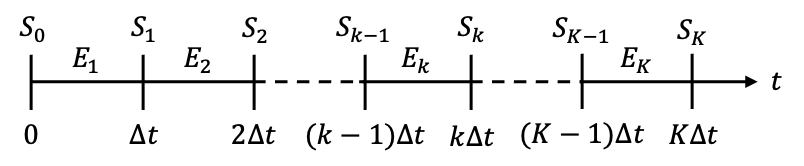
\includegraphics[width=155mm]{../figure/time_dig.png}
 	\caption{Period and measured time (aforementioned)}
 	\label{fig:time_dig_dp}
\end{figure}

\section{本モデルでの状態と行動，状態遷移関数の扱い}
	蓄電池の残量としてとりうる値を，0が最小値， $\overline{b}^{\rm F}$が最大値となるよう，等間隔に $B( \geq 2)$段階で離散化する．これにより， $k$期の末尾における	
	残量 $b_k^{\rm F}$は
	$0,\ \frac{1}{B-1}\overline{b}^{\rm F},\ \frac{2}{B-1}\overline{b}^{\rm F},\ \dots,\ \overline{b}^{\rm F}$のいずれかをとる．
	蓄電池の刻み幅$\Delta b^{\rm F}$を$\Delta b^{\rm F} = \frac{\overline{b}^{\rm F}}{B-1}$と定義する．この定義により蓄電池の残量としてとりうる値は
	$0,\Delta b^{\rm F},2\Delta b^{\rm F},\ \dots,(B-1)\Delta b^{\rm F}$
	と表される．
	また，集合$S_{0},S_{1},\ldots,S_{K}$を以下のように定義する：
	\begin{gather}
	S_k =  \{  s_0 \} ,\quad  k = 0 \\
	S_k = \{ 0, 1, \dots, B - 1 \} ,\quad  k  = 1, \ldots , K．
	 \label{eq:state}
	\end{gather}

	このもとで，集合$S_k$の要素である$s_k$は以下の条件を満たしているものと定義する：
	\begin{equation}
	b_k^{\rm F} = s_k \Delta b^{\rm F}  ,\quad  k  = 0, \ldots , K．
	\label{eq:B_K}
	\end{equation}
	以降，この整数値 $s_k$ を「蓄電池の残量の状態」と呼ぶ．

	電力運用は，各状態における意思決定と，それに伴う状態遷移の繰り返しにより構成される．
	本モデルにおいて，状態$s_{k-1}$で行う意思決定$a_k$を「行動」と呼ぶ．
	ある蓄電池の残量の状態からある行動を実行した際に，次の蓄電池の残量の状態へ遷移する関係を式\eqref{eq:state_transition}のように表し，関数$T$を「状態遷移関数」と呼ぶ．
	\begin{equation}
    		s_k = T(s_{k-1}, a_k) ，\quad  k  =1, \ldots , K
	\label{eq:state_transition}
	\end{equation}	
	本モデルにおける行動$a_k$は，「$k$期の末尾における残量（すなわち次の状態$s_k$）を選択すること」と定義する．
	したがって，$a_k$のとりうる値は蓄電池の残量の状態$s_k$と同様に$0, 1, \dots, B-1$のいずれかとなり，
	式\eqref{eq:state_transition}における状態遷移関数は単純に次のように表される：
	\begin{equation}
		T(s_{k-1}, a_k) = a_k，\quad  k  =1, \ldots , K.
    	\label{eq:state_transition_def}
	\end{equation}
	すなわち，本モデルでは行動$a_k$の決定がそのまま蓄電池の残量の状態$s_k$の決定となる．%この決定に伴い，両状態間の差分として充放電量が計算される．
	

\section{モデルの要素}
モデルの要素(\IS を付して記す)と定数(\IB を付して記す)，変数(\IC を付して表す)を列挙する．
第3章と異なる点として，
\begin{itemize}
	\item 線形計画モデルでは蓄電池の充電量と放電量をそれぞれ独立した非負の変数として定義していたが，
	本モデルではこれらを統合し，正負の値をとる単一の変数として扱っていること
	\item 商用電力系統買電力量が負の値もとりうること
	\item 蓄電池の残量は連続値ではなく，離散化された値をとること
	\item 蓄電池の残量を離散化したときの分割数という定数を導入していること
	\item 蓄電池の残量の状態を表す変数を導入していること
	\item 行動を表す変数を導入していること
\end{itemize}
が挙げられる．モデル中の定数・変数と電力グリッドとの関係を図\ref{fig:variables_dp}に示す．赤色の文字は決定変数，青色の文字は従属変数，緑色の文字は外生変数である．なお，
定数・変数の傍らに灰色で付記された文字は，その定数・変数が当該のケースを採用した場合にのみ現れることを表している．

\begin{itemize}
 	\item[\IS] 太陽光発電設備G
		\begin{itemize}
		 	\item[\IB] 太陽光発電電力量(変換前) $g^{\rm P1}_{k}$
  			\item[\IC] 太陽光発電電力量(変換後) $g^{\rm P2}_{k}$
		\end{itemize}	
	 \item[\IS] 電力消費機器D$^{\rm A}$
	 	\begin{itemize}
		 	\item[\IC] 電力需要量A (変換前) $d^{\rm A1}_{k}$
 			\item[\IB] 電力需要量A (変換後) $d^{\rm A2}_{k}$
		\end{itemize}
 	\item[\IS] 電力消費機器D$^{\rm B}$
	 	\begin{itemize}
		 	\item[\IC] 電力需要量B (変換前) $d^{\rm B1}_{k}$
 			\item[\IB] 電力需要量B (変換後) $d^{\rm B2}_{k}$
		\end{itemize}	
 	\item[\IS] 電力消費機器D$^{\rm C}$
	 	\begin{itemize}
		 	\item[\IC] 電力需要量C (変換前) $d^{\rm C1}_{k}$
 			\item[\IB] 電力需要量C (変換後) $d^{\rm C2}_{k}$
		\end{itemize}
 	\item[\IS] 電力消費機器（自己託送先）D$^{\rm D}$
 	\begin{itemize}
   		\item[\IB] 自己託送先が必要とする電力 $d^{\rm D}$
   		\item[\IB] 自己託送先へ託送することのインセンティブ係数 $p^{\rm D}$   
		\item[\IC] 自己託送先への託送量 (変換前) $d^{\rm D1}_{k}$
 		\item[\IC] 自己託送先への託送量(変換後) $d^{\rm D2}_{k}$
  	\end{itemize} 
 	\item[\IS] 蓄電池B$^{\rm F}$
  		\begin{itemize}
   			\item[\IB] 蓄電池の最大容量 $\overline{b}^{\rm F}$
			\item[\IB] 蓄電池の残量の初期状態$s_{0}$
			\item[\IC] 蓄電池の残量の状態$s_{k}$
			\item[\IC] 行動$a_{k}$
			\item[\IB] 蓄電池の残量を離散化したときの分割数$B$
			\item[\IB] 蓄電池の残量の初期状態$b^{\rm F}_{0}$
		  	\item[\IC] 蓄電池の(期末の)残量 $b^{\rm F}_{k}$
  			\item[\IC] 蓄電池の残量の状態$s_{k-1}$で行動$a_{k}$を行なった際の蓄電池の充電量(変換前) $x^{\rm FC1}_{k}(s_{k-1},a_{k})$\\
			ただし，$x^{\rm FC1}_{k}(s_{k-1},s_{k}) < 0$を満たしているときは$|x^{\rm FC1}_{k}(s_{k-1},a_{k})|$だけ放電を行っていると解釈する．
  			\item[\IC] 蓄電池の残量の状態$s_{k-1}$で行動$a_{k}$を行なった際の蓄電池の充電量(変換後) $x^{\rm FC2}_{k}(s_{k-1},a_{k})$\\
			ただし，$x^{\rm FC2}_{k}(s_{k-1},a_{k}) < 0$を満たしているときは$|x^{\rm FC2}_{k}(s_{k-1},a_{k})|$だけ放電を行っていると解釈する．
			 \item[\IB] 単位時間あたりの最大充電電量 $a^{\rm FC}$
  			\item[\IB] 単位時間あたりの最大充放電量 $a^{\rm FD}$
  		\end{itemize}
 	\item[\IS] 電力変換装置(太陽光) E$^{\rm P}$
  		\begin{itemize}
   			\item[\IB] 変換効率 $\alpha^{\rm P}$
  		\end{itemize}
 	\item[\IS] 電力変換装置(商用電力系統) E$^{\rm S}$
 	\item[\IS] 電力変換器(消費機器A) E$^{\rm DA}$
  		\begin{itemize}
   			\item[\IB] 変換効率 $\alpha^{\rm DA}$
 		\end{itemize}
 	\item[\IS] 電力変換器(消費機器B) E$^{\rm DB}$
  		\begin{itemize}
  	 		\item[\IB] 変換効率 $\alpha^{\rm DB}$
 	 	\end{itemize}
 	\item[\IS] 電力変換器(消費機器C) E$^{\rm DC}$
	  	\begin{itemize}
	   		\item[\IB] 変換効率 $\alpha^{\rm DC}$
	 	 \end{itemize}
  	\item[\IS] 電力変換器(消費機器D) E$^{\rm DD}$
  	\begin{itemize}
   		\item[\IB] 変換効率 $\alpha^{\rm DD}$
  	\end{itemize} 
	
 	%\item[\IS] 蓄電池の自己放電に相当する仮想的な変換器 Z$^{ -1}$
  		%\begin{itemize}
   			%\item[\IB] 期$k$の先頭から期$k$の末尾にかけての自己放電効率$\alpha^{\rm FT}$
  		%\end{itemize}
 	\item[\IS] 電力変換器(蓄電池)E$^{\rm BF}$
  		\begin{itemize}
   			\item[\IB] 充電効率 $\alpha^{\rm FC}$
   			\item[\IB] 放電効率 $\alpha^{\rm FD}$
  		\end{itemize}
 	\item[\IS] 商用電力系統S
   		\begin{itemize}
		  	\item[\IC] 蓄電池の残量の状態$s_{k-1}$で行動$a_{k}$を行なった際の商用電力系統買電力量$s^{\rm BY}_{k}(s_{k-1},a_{k})$\\
			ただし，$s^{\rm BY}_{k}(s_{k-1},a_{k}) < 0$を満たしているときは$|s^{\rm BY}_{k}(s_{k-1},a_{k})|$だけ系統に売電，あるいは
			自己託送先に託送を行なっている，あるいは無駄電力が生ずると解釈する．
   			\item[\IB] 系統電力量料金単価 $p^{\rm BY}_{k}$
   			\item[\IB] 系統基本料金単価 $p^{\rm BYMax}$
   			\item[\IB] 系統売電単価 $p^{\rm SL}_{k}$
   			%\item[\IB] 単位時間あたりの最大系統売電量 $a^{\rm SL}_{k}$
  		\end{itemize}
 	\item[\IS] 工場外の空間O
\end{itemize}

\begin{figure}[h]
 \centering
 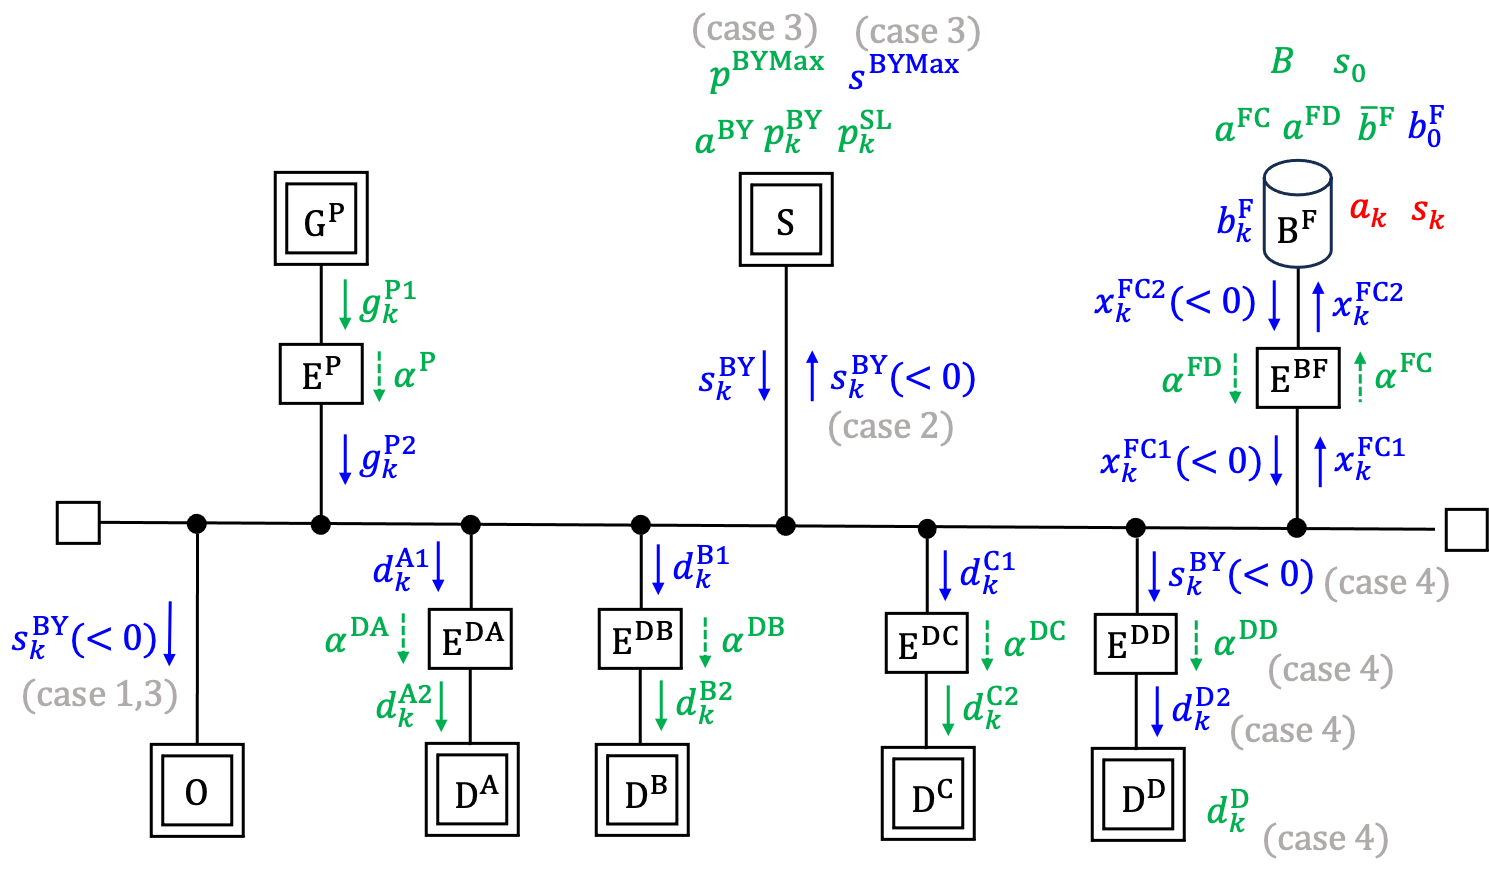
\includegraphics[width=140mm]{../figure/variables_dp.png}
 \caption{Configuration diagram of the target system(Dynamic Programming)}
 \label{fig:variables_dp}
\end{figure}

\section{定数・変数どうしの関係式}
\begin{itemize}
	\item 動線\\
		流入する電力と流出する電力の総和が等しいものとする．
		\begin{equation}
 			s_k^{\rm BY}(s_{k-1},a_{k})= 
	 		d_k^{\rm A1}+ d_k^{\rm B1} + d_k^{\rm C1}+  x_k^{\rm FC1}(s_{k-1},a_{k}) - g_k^{\rm P2},  \quad k=1,\ldots,K
 		 \label{eq:line_dp}
		\end{equation}
	\item 蓄電池\\
		蓄電池の残量は常に定められた範囲内を外れないこと，なおかつ，単位時間あたりの充放電電力は，最大出力を超過しないこと．
		\begin{equation}
       		 \label{eq:line_action_restrict}
        		\begin{split}
            		& a_k \in A_k(s_{k-1}), \\
            		& A_k(s_{k-1}) = \{ s_{k-1} + \Delta s_k^{\mathrm{Min}}(s_{k-1}),s_{k-1} + \Delta s_k^{\mathrm{Min}}(s_{k-1})+1, \dots, s_{k-1} + \Delta s_k^{\mathrm{Max}}(s_{k-1}) \},\\
            		& k=1,\dots,K
        		\end{split}
    		\end{equation}
    		ここで，$\Delta s_k^{\mathrm{Min}}(s_{k-1})$ および $\Delta s_k^{\mathrm{Max}}(s_{k-1})$ は，
		それぞれ状態 $s_{k-1}$ において許容される残量の最大放電量および最大最大充電量に相当する，添字を返す関数である．
		
		
	\item 電力変換装置\\
		パワーコンディショナや変圧器などを介して電力を変換・送電する際，一定の変換効率に応じた電力損失が発生するものとする．
		\begin{equation}
 			g^{\rm P2}_{k} = \alpha^{\rm P} g^{\rm P1}_{k} ,  \quad k=1,\ldots,K
		\label{eq:gP1gP2_dp}
		\end{equation}
		%
		\begin{equation}
 			d^{\rm A2}_{k} = \alpha^{\rm DA} d^{\rm A1}_{k} ,\quad k=1,\ldots,K
		 \label{eq:dA1A2_dp}
		\end{equation}
		%
		\begin{equation}
 			d^{\rm B2}_{k} = \alpha^{\rm DB} d^{\rm B1}_{k},\quad k=1,\ldots,K
 		\label{eq:dB1B2_dp}
		\end{equation}
		%
		\begin{equation}
 			d^{\rm C2}_{k} = \alpha^{\rm DC} d^{\rm C1}_{k},\quad k=1,\ldots,K
 		\label{eq:dC1C2_dp}
		\end{equation}
		%
		\begin{equation}
 			x^{\rm FC2}_{k}(s_{k-1},a_{k}) =\begin{cases}
  			\alpha^{\rm FC}x^{\rm FC1}_{k}(s_{k-1},a_{k})  \quad \text{if } a_k-s_{k-1} \ge 0 \\
 			 \frac{1}{\alpha^{\rm FD}}x^{\rm FC1}_{k}(s_{k-1},a_{k}) \quad \text{otherwise }
			 \end{cases},
  			\quad k=1,\ldots,K
 		\label{eq:xFC1FC2_dp}
		\end{equation}

		%
		ケース4において$s^{\rm BY}_{k} < 0$を満たす場合
		\begin{equation}
 			d^{\rm D2}_{k} = -\alpha^{\rm DC} s^{\rm BY}_{k}(s_{k-1},a_{k}),\quad k=1,\ldots,K
 		\label{eq:dD1D2_dp}
		\end{equation}
	
\end{itemize}

\section{評価関数と目的関数}
	第3章の目的関数と対応させるべく，本モデルにおける最適化の目的は，全期間を通じた電力運用コストを最小化することとする．
	これを動的計画法で扱うために，各期間ごとに発生するコストを「評価関数」として定義し，
	その総和を最小化する問題として定式化する．
	蓄電池の残量の状態 $s_{k-1}$において行動$a_{k}$を行なった際の評価関数を$R_k(s_{k-1},a_{k})$とする．
	この評価関数は，制約条件を満たす行動 $a_k \in A_{k}(s_{k-1})$ が選択されたときにのみ定義される．
	蓄電池の残量の状態や行動，状態遷移，評価関数の関係を可視化したものを図\ref{fig:network}に示す．
	このとき，目的関数は
	\begin{figure}[h]
 		\centering
 		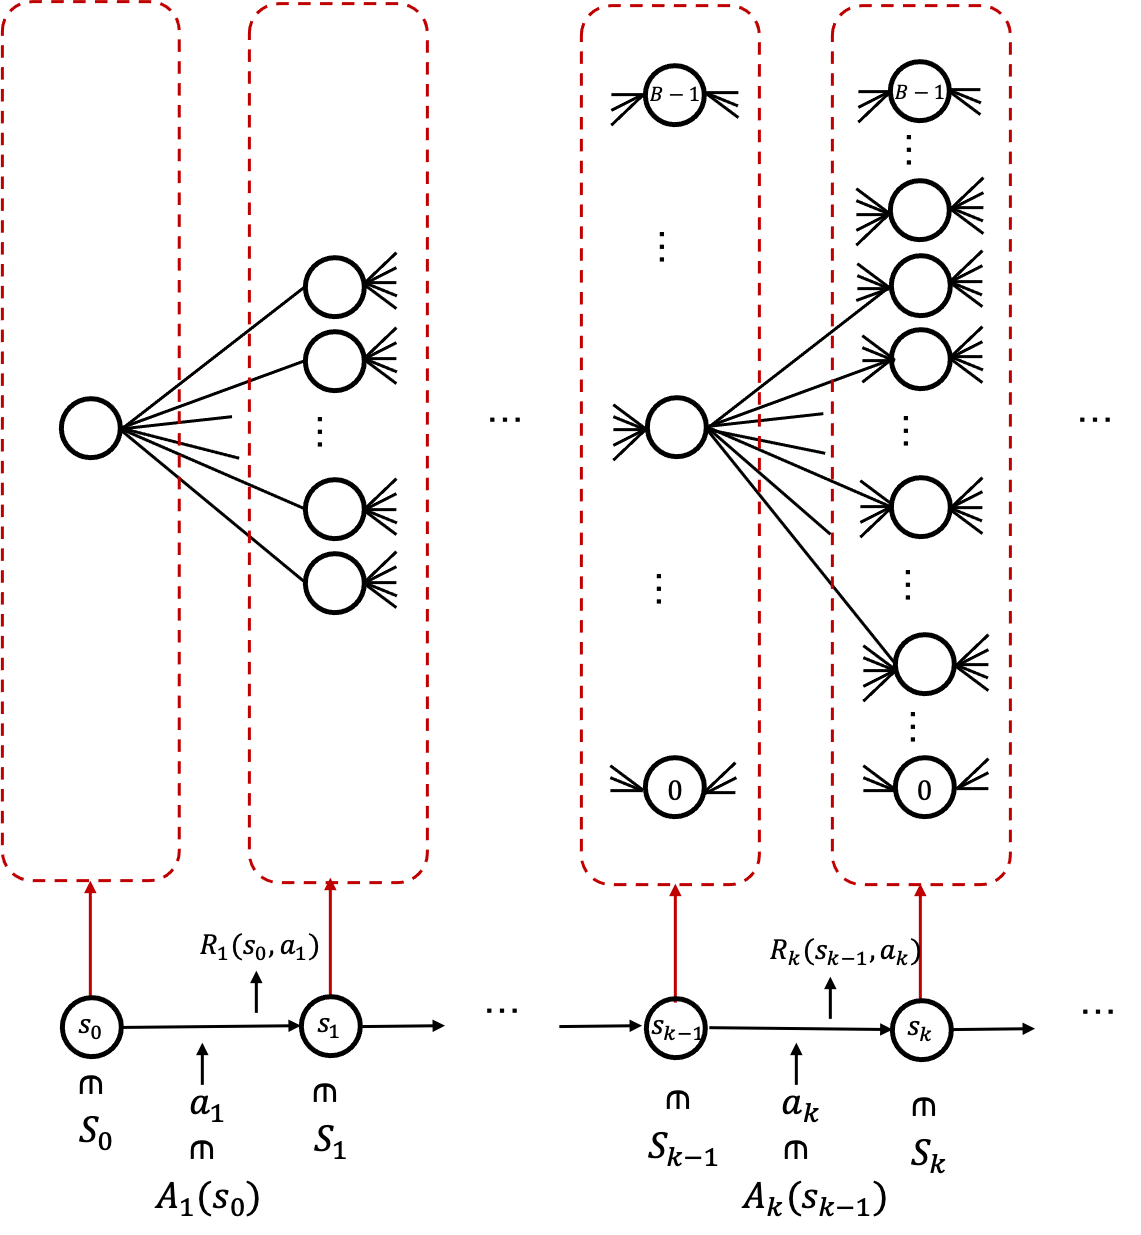
\includegraphics[width=145mm]{../figure/network.png}
 		\caption{image of state transition}
		 \label{fig:network}
	\end{figure}

	\begin{equation}
		\text{Minimize} \quad  \sum_{k=1}^{K-1} R_k(s_{k-1},a_{k}) \quad  a_{k}\in A_k({s_{k-1})}
 	\label{eq:minimize_dp}
	\end{equation}
	と表される．
	以下，評価関数の定式化の方法について述べる．評価関数の定義にはいくつかの方法が考えられるが，
	本節では3.3節で示した目的関数と対応させる形でケース1，ケース2，およびケース4の評価関数を定式化する．
	なおケース3については，0期から現在の期までの買電量の最大値を記憶しておかなければならず，最適性の原理を満足する形で定式化を行う際は
	状態空間の次元を拡張する必要があり，時間的計算量が膨大になる．よってこのケースについては本研究の対象外とするが，
	ケース3の時間的計算量についての考察は付録に記載する．

\subsection{ケース1の場合}\label{sec:R}
	$s^{\rm BY}_{k}(s_{k-1},a_{k}) < 0$を満たしているときは$|s^{\rm BY}_{k}(s_{k-1},a_{k})|$だけ無駄電力が生ずるとする
	点に注意すると，評価関数は以下のように表される：

	\begin{equation}
		R_k(s_{k-1},a_{k}) = p_k^{\rm BY} \max (s_k^{\rm BY}(s_{k-1},a_{k}) , 0).
 		\label{eq:R_1}
	\end{equation}	
	このケースでは売電を考慮しないため$s_k^{\rm BY}(s_{k-1},a_{k})$が負となる場合，
	$\max (s_k^{\rm BY}(s_{k-1},a_{k}) , 0)$の値は0となる．
	
	ここで，式\eqref{eq:line_dp}より，式\eqref{eq:R_1}は次のように書き換えられる：
	\begin{equation}
		R_k(s_{k-1},a_{k}) = p_k^{\rm BY} \max (d_k^{\rm A1}+ d_k^{\rm B1} + d_k^{\rm C1}+  x_k^{\rm FC1}(s_{k-1},a_{k}) - g_k^{\rm P2} , 0).
 		\label{eq:R_1_2}
	\end{equation}	
	また，式\eqref{eq:xFC1FC2_dp}より式\eqref{eq:R_1_2}は次のように表される．
	\begin{equation}
		R_k(s_{k-1},a_{k}) = p_k^{\rm BY} \max (d_k^{\rm A1}+ d_k^{\rm B1} + d_k^{\rm C1}+  \frac{x_k^{\rm FC2}(s_{k-1},a_{k})}{\alpha^{\rm FC}} - g_k^{\rm P2} , 0).
 		\label{eq:R_1_3}
	\end{equation}	
	ところで，式\eqref{eq:B_K}より$x_k^{\rm FC2}(s_{k-1},a_{k})$は
	\begin{equation}
		x_k^{\rm FC2}(s_{k-1},a_{k}) = (a_{k} - s_{k-1})\Delta b^{\rm F}
		\label{eq:FC2_state}
	\end{equation}
	と表され，この式\eqref{eq:FC2_state}を用いることで式\eqref{eq:R_1_3}は次のように表される：
	\begin{equation}
		R_k(s_{k-1},a_{k}) = p_k^{\rm BY} \max (d_k^{\rm A1}+ d_k^{\rm B1} + d_k^{\rm C1}+  \frac{(a_{k} - s_{k-1})\Delta b^{\rm F}}{\alpha^{\rm FC}} - g_k^{\rm P2} , 0).
 		\label{eq:R_1_4}
	\end{equation}		
	\eqref{eq:R_1_4}の右辺に含まれる $p_k^{\rm BY},d_k^{\rm B1},d_k^{\rm C1},\Delta b^{\rm F},\alpha^{\rm FC},g_k^{\rm P2}$は
	外生変数なので，遷移可能な全ての状態遷移について評価関数を設定することができる．
	
\subsection{ケース2の場合}
$s^{\rm BY}_{k}(s_{k-1},a_{k}) < 0$を満たしているときは$|s^{\rm BY}_{k}(s_{k-1},a_{k})|$だけ系統に売電するとする点に注意すると，
評価関数は以下のように表される：

\begin{equation}
  %w_{k-1}(s_{i},s_{j}) = p_k^{\rm BY/SL} \left[ \frac{j - i}{n-1} \cdot \overline{b} - \{ g_k^{\rm P2} - (d_k^{\rm A2} + d_k^{\rm B2} + d_k^{\rm C2}) \} \right]．
  %s_k^{\rm{BYMinIDX}} \le j-i \le s_k^{\rm{BYMaxIDX}}
  R_{k}(s_{k-1},a_{k}) = \begin{cases}
   p_k^{\rm BY}s_k^{\rm BY}(s_{k-1},a_{k}),\quad   \text{if } s_k^{\rm BY}(s_{k-1},a_{k}) \ge 0\\
   -p_k^{\rm SL}s_k^{\rm BY}(s_{k-1},a_{k}),\quad \text{otherwise}．
   \end{cases}
 \label{eq:R_2}
\end{equation}

この式\eqref{eq:R_2}に対して\ref{sec:R}節と同様の方法で変形を施すと次のようになる：
\begin{equation}
	R_{k}(s_{k-1},a_{k}) = \begin{cases}
	  p_k^{\text{BY}} \{d_k^{\text{A1}}+ d_k^{\text{B1}} + d_k^{\text{C1}}+  \frac{(a_{k} - s_{k-1})\Delta b^{\text{F}}}{\alpha^{\text{FC}}} - g_k^{\text{P2}} \} \\
	  \hfill \text{if } d_k^{\text{A1}}+ d_k^{\text{B1}} + d_k^{\text{C1}}+  \frac{(a_{k} - s_{k-1})\Delta b^{\text{F}}}{\alpha^{\text{FC}}} - g_k^{\text{P2}}  \ge 0 \\[1ex]
	  -p_k^{\text{SL}} \{d_k^{\text{A1}}+ d_k^{\text{B1}} + d_k^{\text{C1}}+  \alpha^{\text{FD}}(a_{k} - s_{k-1})\Delta b^{\text{F}} - g_k^{\text{P2}} \} \\
	  \hfill \text{otherwise.}
	\end{cases}
\label{eq:R_2_1}
\end{equation}
\eqref{eq:R_2_1}の右辺に含まれる $p_k^{\rm BY},d_k^{\rm B1},d_k^{\rm C1},\Delta b^{\rm F},\alpha^{\rm FC},\alpha^{\rm FD},g_k^{\rm P2}$は
	外生変数なので，遷移可能な全ての状態遷移について評価関数を設定することができる．
	
\subsection{ケース4の場合}
$s^{\rm BY}_{k}(s_{k-1},a_{k}) < 0$を満たしているときは$|s^{\rm BY}_{k}(s_{k-1},a_{k})|$だけ自己託送をするとする点に注意すると，
評価関数は以下のように表される．
\begin{equation}
  %w_{k-1}(s_{i},s_{j}) = p_k^{\rm BY/SL} \left[ \frac{j - i}{n-1} \cdot \overline{b} - \{ g_k^{\rm P2} - (d_k^{\rm A2} + d_k^{\rm B2} + d_k^{\rm C2}) \} \right]．
  %s_k^{\rm{BYMinIDX}} \le j-i \le s_k^{\rm{BYMaxIDX}}
  	R_{k}(s_{k-1},a_{k}) = \begin{cases}
   		p_k^{\rm BY}s_k^{\rm BY}(s_{k-1},a_{k}),\quad   \text{if } s_k^{\rm BY}(s_{k-1},a_{k}) \ge 0\\
   		-p_k^{\rm D}d_k^{\rm D2} ，\text{otherwise}．
  	\end{cases}
 \label{eq:R_3}
\end{equation}
式\eqref{eq:dD1D2_dp}より式\eqref{eq:R_3}は次のように書き換えられる：
\begin{equation}
  %w_{k-1}(s_{i},s_{j}) = p_k^{\rm BY/SL} \left[ \frac{j - i}{n-1} \cdot \overline{b} - \{ g_k^{\rm P2} - (d_k^{\rm A2} + d_k^{\rm B2} + d_k^{\rm C2}) \} \right]．
  %s_k^{\rm{BYMinIDX}} \le j-i \le s_k^{\rm{BYMaxIDX}}
  	R_{k}(s_{k-1},a_{k}) = \begin{cases}
   		p_k^{\rm BY}s_k^{\rm BY}(s_{k-1},a_{k}),\quad   \text{if } s_k^{\rm BY}(s_{k-1},a_{k}) \ge 0\\
   		-p_k^{\rm D}(-\alpha^{\rm DD} s^{\rm BY}_{k}(s_{k-1},a_{k})) ，\text{otherwise}．
  	\end{cases}
 \label{eq:R_3_1}
\end{equation}
この式\eqref{eq:R_3_1}に対して\ref{sec:R}と同様の方法で変形を施すと次のようになる：
\begin{equation}
R_{k}(s_{k-1},a_{k}) = \begin{cases}
    p_k^{\mathrm{BY}} \{d_k^{\text{A1}}+ d_k^{\text{B1}} + d_k^{\text{C1}}+  \frac{(a_{k} - s_{k-1})\Delta b^{\text{F}}}{\alpha^{\text{FC}}} - g_k^{\text{P2}} \} \\
    \hfill \text{if } d_k^{\text{A1}}+ d_k^{\text{B1}} + d_k^{\text{C1}}+  \frac{(a_{k} - s_{k-1})\Delta b^{\text{F}}}{\alpha^{\text{FC}}} - g_k^{\text{P2}}  \ge 0 \\[2ex]
    -p_k^{\mathrm{D}} [-\alpha^{\mathrm{DD}} \{d_k^{\text{A1}}+ d_k^{\text{B1}} + d_k^{\text{C1}}+  \alpha^{\text{FD}}(a_{k} - s_{k-1})\Delta b^{\text{F}} - g_k^{\text{P2}} \}] \\
    \hfill \text{otherwise.}
\end{cases}
\label{eq:R_3_2}
\end{equation}
\eqref{eq:R_3_2}の右辺に含まれる $p_k^{\rm BY},d_k^{\rm B1},d_k^{\rm C1},\Delta b^{\rm F},\alpha^{\rm FC},\alpha^{\rm FD},\alpha^{\rm DD},g_k^{\rm P2}$は
	外生変数なので，遷移可能な全ての状態遷移について評価関数を設定することができる．


\section{最適性の原理}
	問題を動的計画法で解くためには，目的関数が分離可能性と単調性を満たせばよい\cite{h}．
	分離可能性とは，$i$番目から$n$番目までの引数のみに依存する目的関数を$F_i(r_i,\dots,r_n)$
	としたときに，その目的関数が
	\begin{equation}
		F_i(r_i,\dots,r_n) = F_i(r_i,f_{i+1}(r_{i+1},\dots,r_n))
		\label{eq:dp_bunri}
	\end{equation}
	と表されることを指す．単調性とは，$F_i(r_i,F_{i+1})$が$F_{i+1}$に関して単調であることを表す．
	
	以下，本問題がこれらの性質を満たすことを示す．
	 本問題における目的関数を，評価関数の引数を省略して$F_{0}(R_0,R_1,\dots,R_{K})$と表すことにする．
	このとき，この目的関数の部分和である，$i$期から$K$期までの評価関数の累積和を$F_{i}(R_i,R_{i+1},\dots,R_{K})$と表すことにすると，
	\begin{equation}
		F_{i}(R_i,R_{i+1},\dots,R_{K}) = R_i+ R_{i+1}+\dots+R_{K}
		\label{eq:F_i}
	\end{equation}
	となる．式\eqref{eq:F_i}は
	\begin{equation}
		F_{i}(R_i,R_{i+1},\dots,R_{K}) = R_{i} + F_{i+1}(R_{i+1},R_{i+2},\dots,R_{K})
		\label{eq:F_i2}
	\end{equation}	
	と書き換えられる．式\eqref{eq:F_i2}の右辺の形から本問題の目的関数は分離可能性を満たす．
	次に単調性について確認する．式\eqref{eq:F_i2}において，$F_{i+1}$の係数は正の定数である．
	したがって，$F_{i+1}$の値が増加すれば$F_i$の値も増加する．
	すなわち，$F_i$は$F_{i+1}$に関して単調非減少であるため，単調性を満たす．
	以上より，本問題は分離可能性と単調性を満たしており，最適性の原理が成立するため，動的計画法により解くことができる．
	
\section{Bellman方程式}
	$F_{k}^{*}(s_k)$ を，$k$期の末尾において蓄電池の残量の状態が $s_k$ であるとき，それ以降の期（$k+1$ 期から $K$ 期まで）に
	発生する評価値の累積和の最小値と定義する．すなわち，
	\begin{equation}
		F_{k}^{*}(s_{k}) = \min \sum_{l=k+1}^{K} R_l(s_{l-1}, a_{l}) \quad a_l \in A_l(s_{l-1})
	\end{equation}
	と表される．このとき，最適性の原理に基づき，$F_{k-1}^{*}(s_{k-1})$ は，
	以下のBellman方程式によって再帰的に求めることができる．
	\begin{equation}
		F_{k-1}^{*}(s_{k-1}) = \min_{a_k \in A_k(s_{k-1})} { R_k(s_{k-1}, a_k) + F_{k}^{*}(a_k) }
		\label{eq:bellman_backward}
	\end{equation}
	ただし$K$期の末尾における評価値は次のように与えられる．
	\begin{equation}
		F_{K}^{*}(s_{K}) = 0,\quad \forall s_K \in S_K
	\end{equation}
	式 \eqref{eq:bellman_backward} において，行動 $a_k$ の決定は式 \eqref{eq:state_transition_def} より蓄電池の残量の次の状態 $s_k$ の決定と等価であるため，
	右辺第2項の $F_k^{*}$ の引数は $a_k$ となっている．この方程式を $k=K$ から $1$ へと逆方向に順次適用することで，
	各時刻・蓄電池の残量の各状態における最適な行動選択と最小コストを算出できる．最終的に，初期状態 $s_0$ に対する $F_0^*(s_0)$ を求めることで，
	全期間における最小の評価値の総和が得られる．



%計算例
%!TEX root = ../main.tex

\chapter{計算例}
本章では，例題を用いて計算を行った結果を示し，本研究で作成した2つの数理モデルの妥当性や有用性について検討する.
なお，求解には最適化ソルバーとしてpySCIPOptを用いた\cite{x}．

\section{問題設定}
高知県内の某工場を対象に電力運用最適化モデルを導入し，2025 年7月3日木曜日0時00分から7月9日水曜日23時59分までの1週間についての運用計画を考えるケースを想定する．
各々の期の刻み幅$\Delta t$は1分とする．
このとき，$K = 60 \times 24 \times 7 = 10080$となる．
本例題では，工場側から「余剰電力の売電を考慮し，正味の支出を最小化したい」という要求があるものとし，
ケース2に基づいて検討を行う．

\subsection{太陽光発電設備}
1週間先までの太陽光発電量の予測値が，1分刻みの時系列データとして与えられているものとし，
これを$g_k^{\rm P1}$に代入する．
本計算例における$g_k^{\rm P1}$の値を図\ref{fig:lp_gP1}に示す．
なお，以降の折れ線グラフにおいて，赤色は決定変数，青色は従属変数，緑色は外生変数を表すものとする．
\begin{figure}[h]
	\centering
 	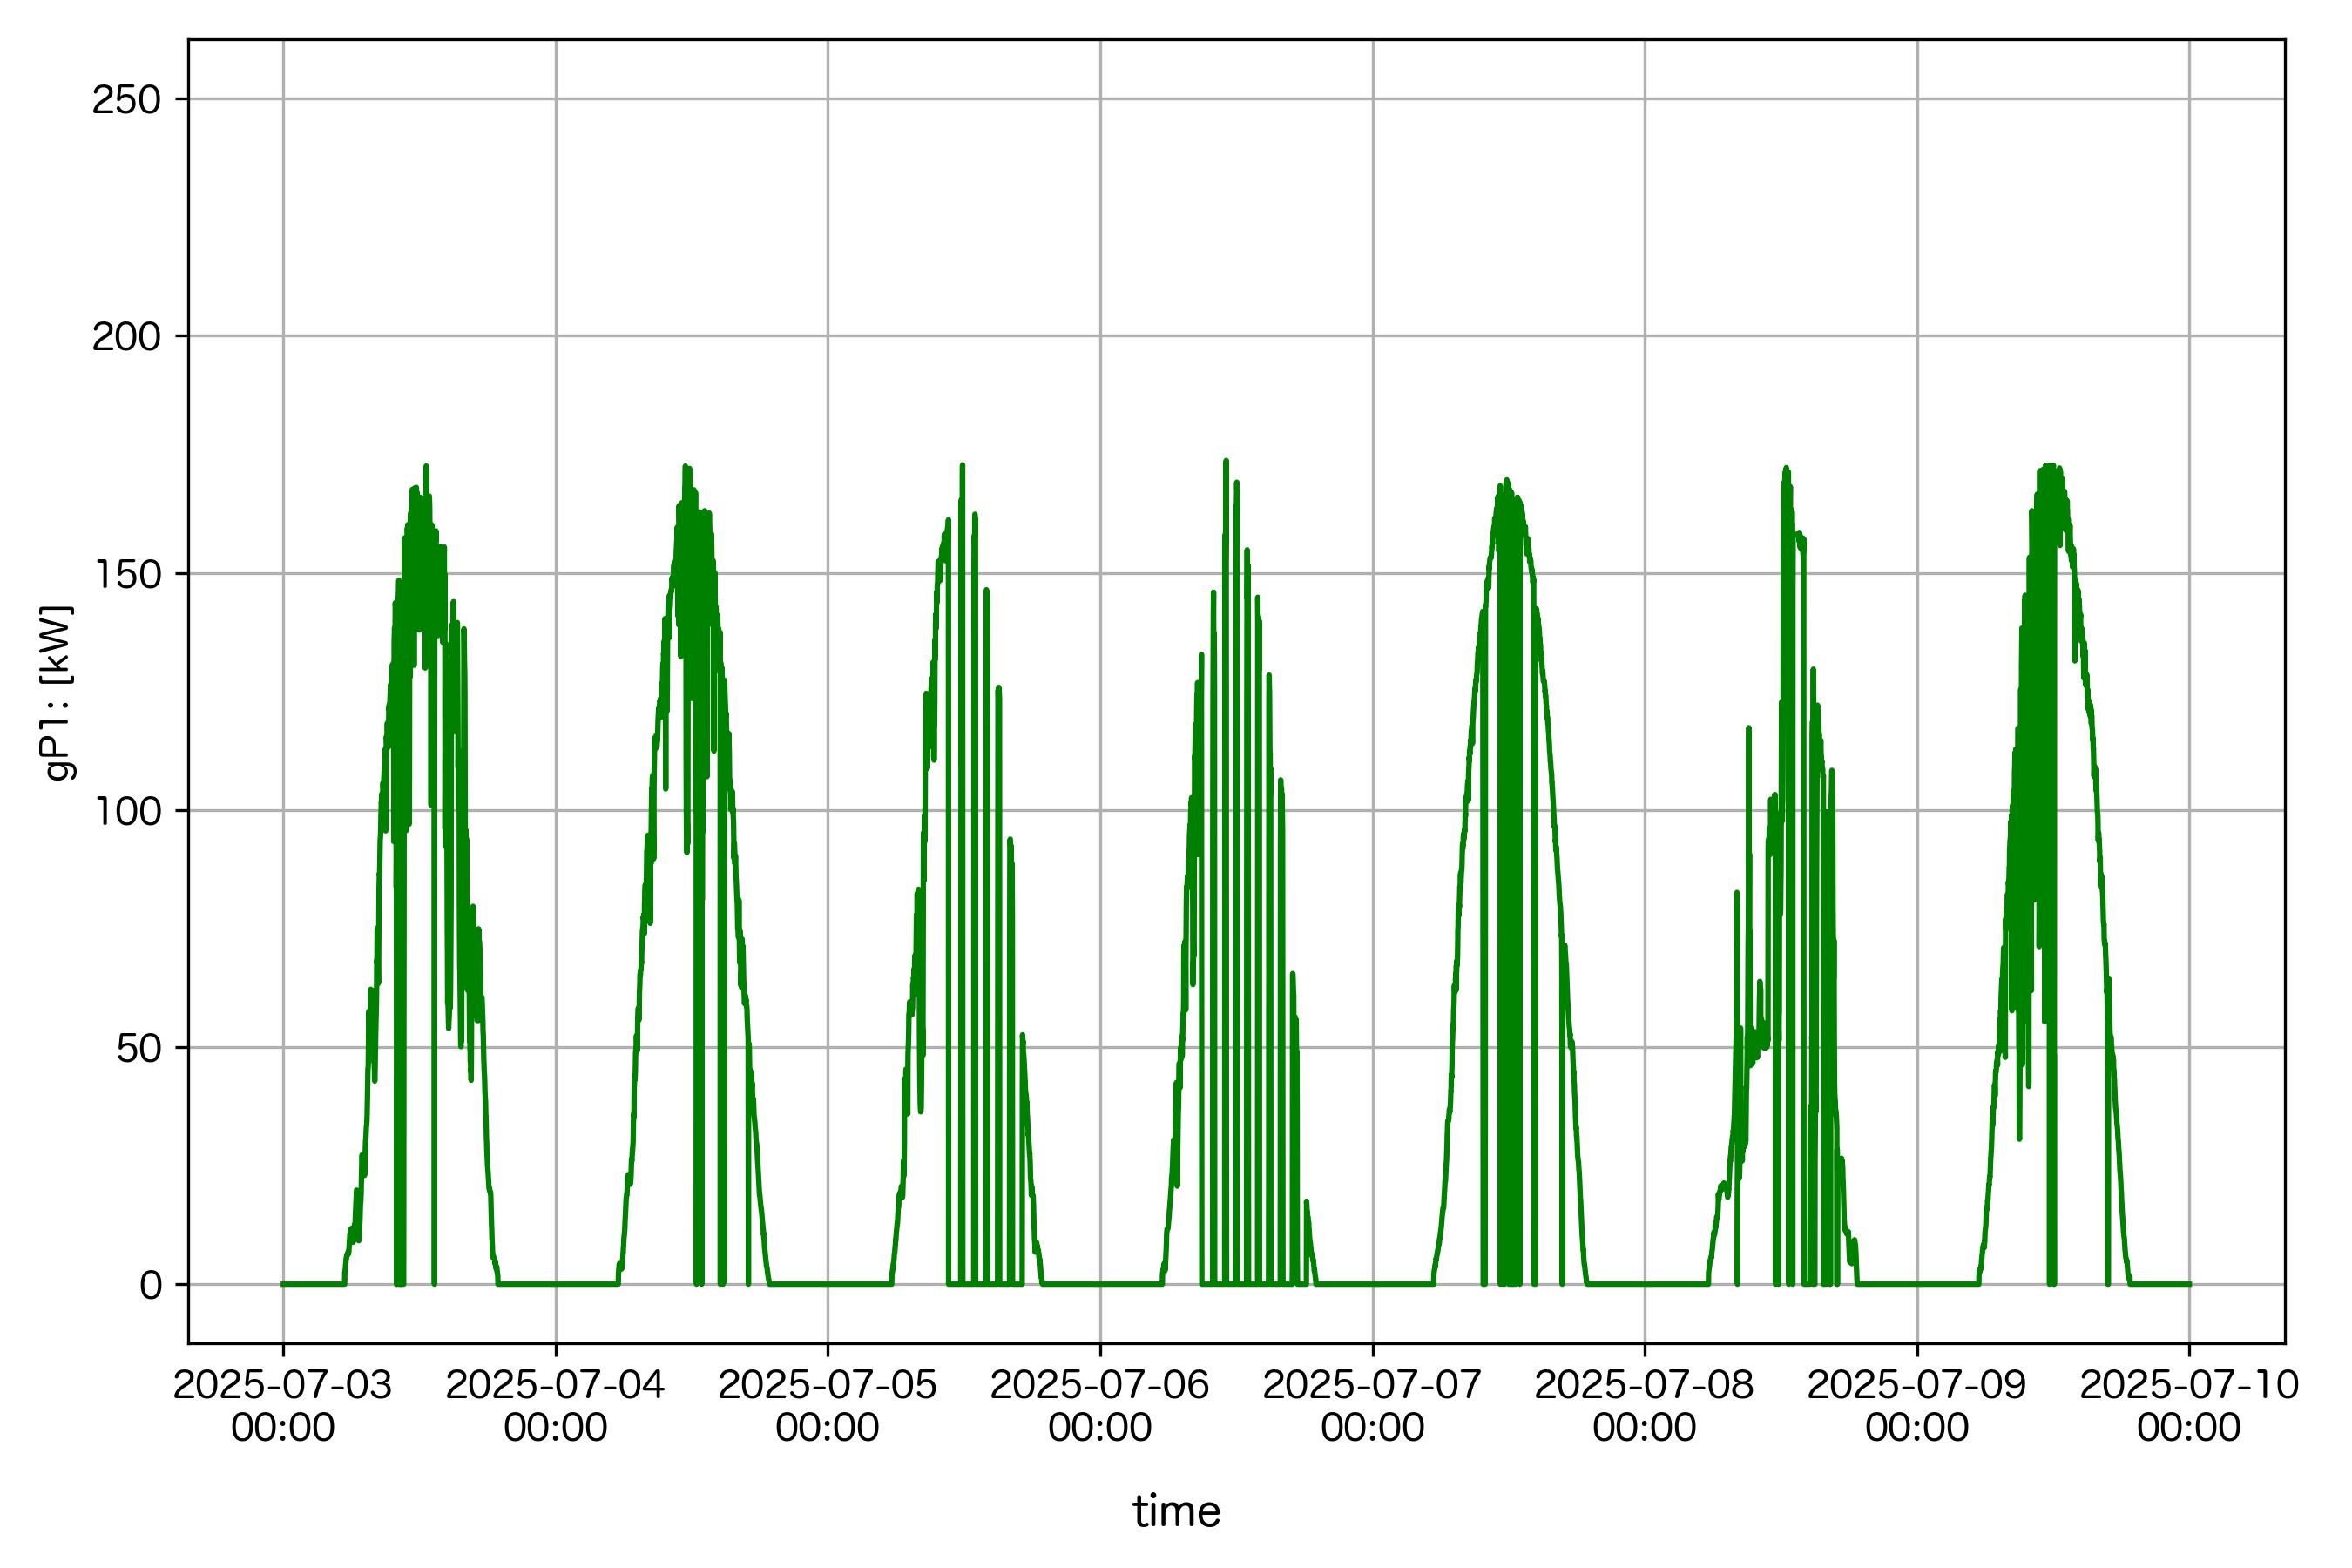
\includegraphics[width=120mm]{../figure/lp/gP1.png}
 	\caption{Solar PV Generation (Before Conversion)}
 	\label{fig:lp_gP1}
\end{figure}

\subsection{電力消費機器}
1週間先までの電力消費機器の電力消費量の予測値が，1分刻みの時系列データとして与えられているものとし，
これを$d_k^{\rm DA},d_k^{\rm DB},d_k^{\rm DC}$に代入する．
本計算例における$d_k^{\rm DA},d_k^{\rm DB},d_k^{\rm DC}$の値を図\ref{fig:lp_dA2}〜図\ref{fig:lp_dC2}に示す．
\begin{figure}[h]
	\centering
 	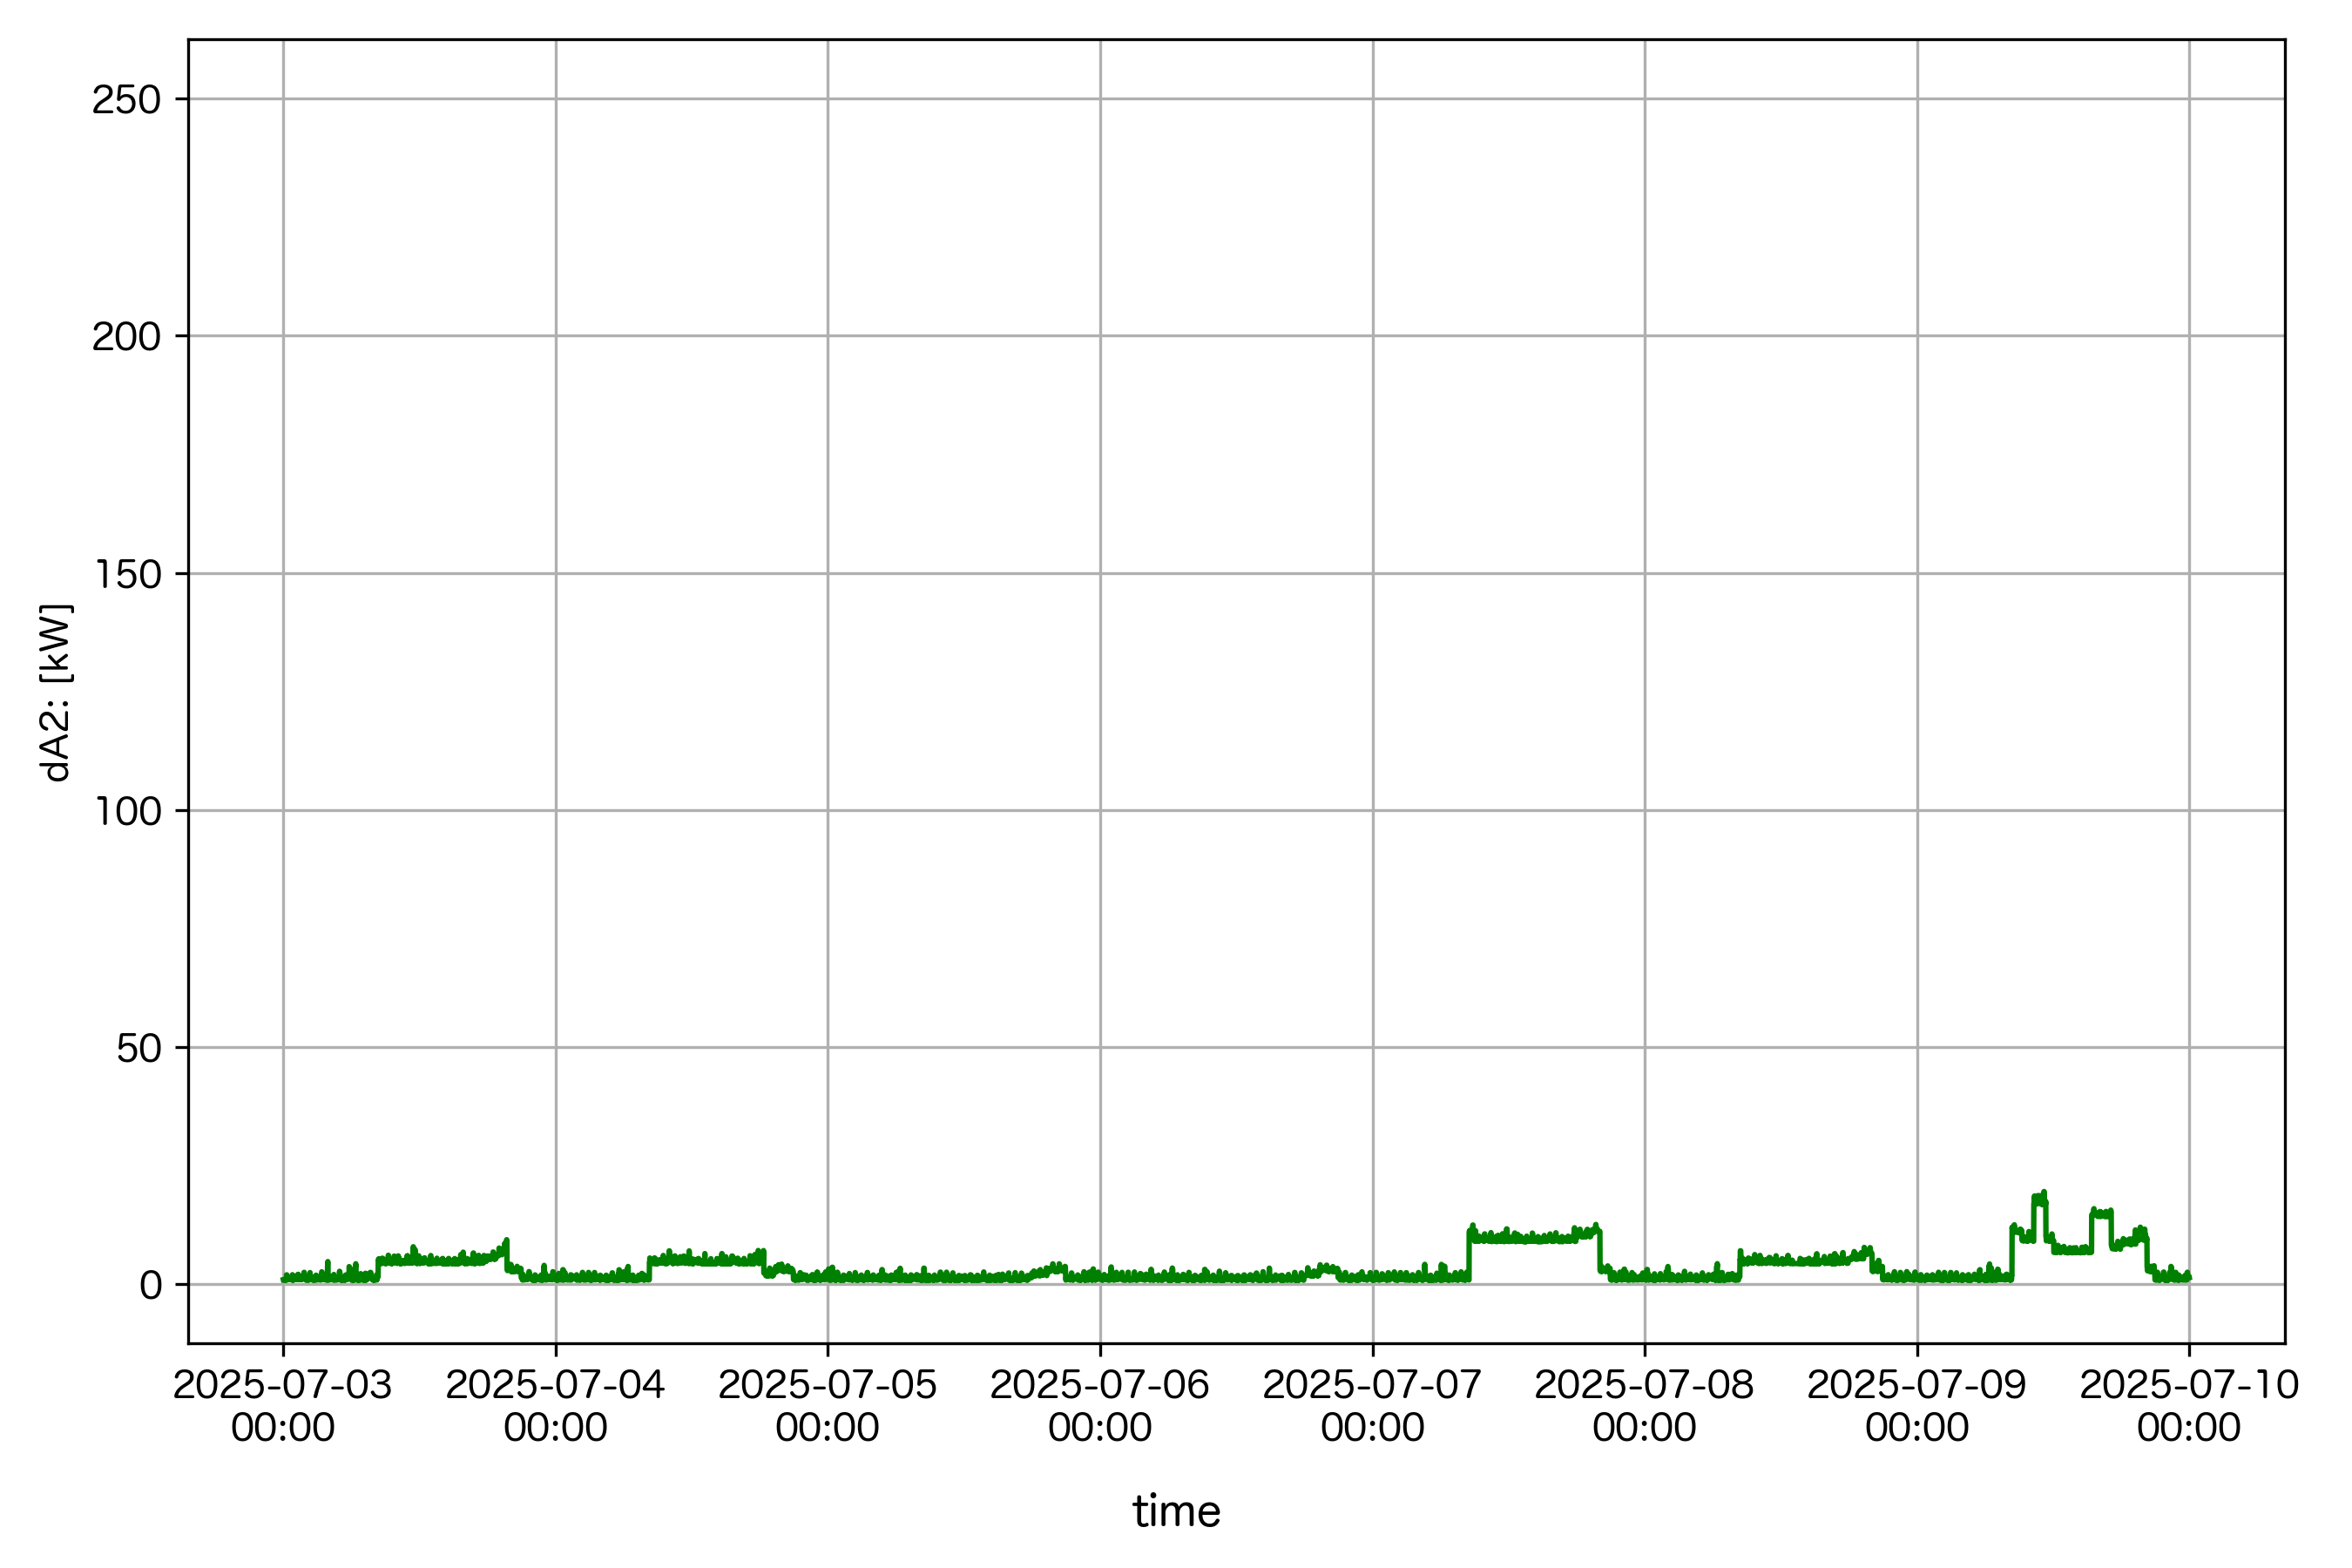
\includegraphics[width=120mm]{../figure/lp/dA2.png}
 	\caption{Power Consumption A (After Conversion)}
 	\label{fig:lp_dA2}
\end{figure}
\begin{figure}[h]
	\centering
 	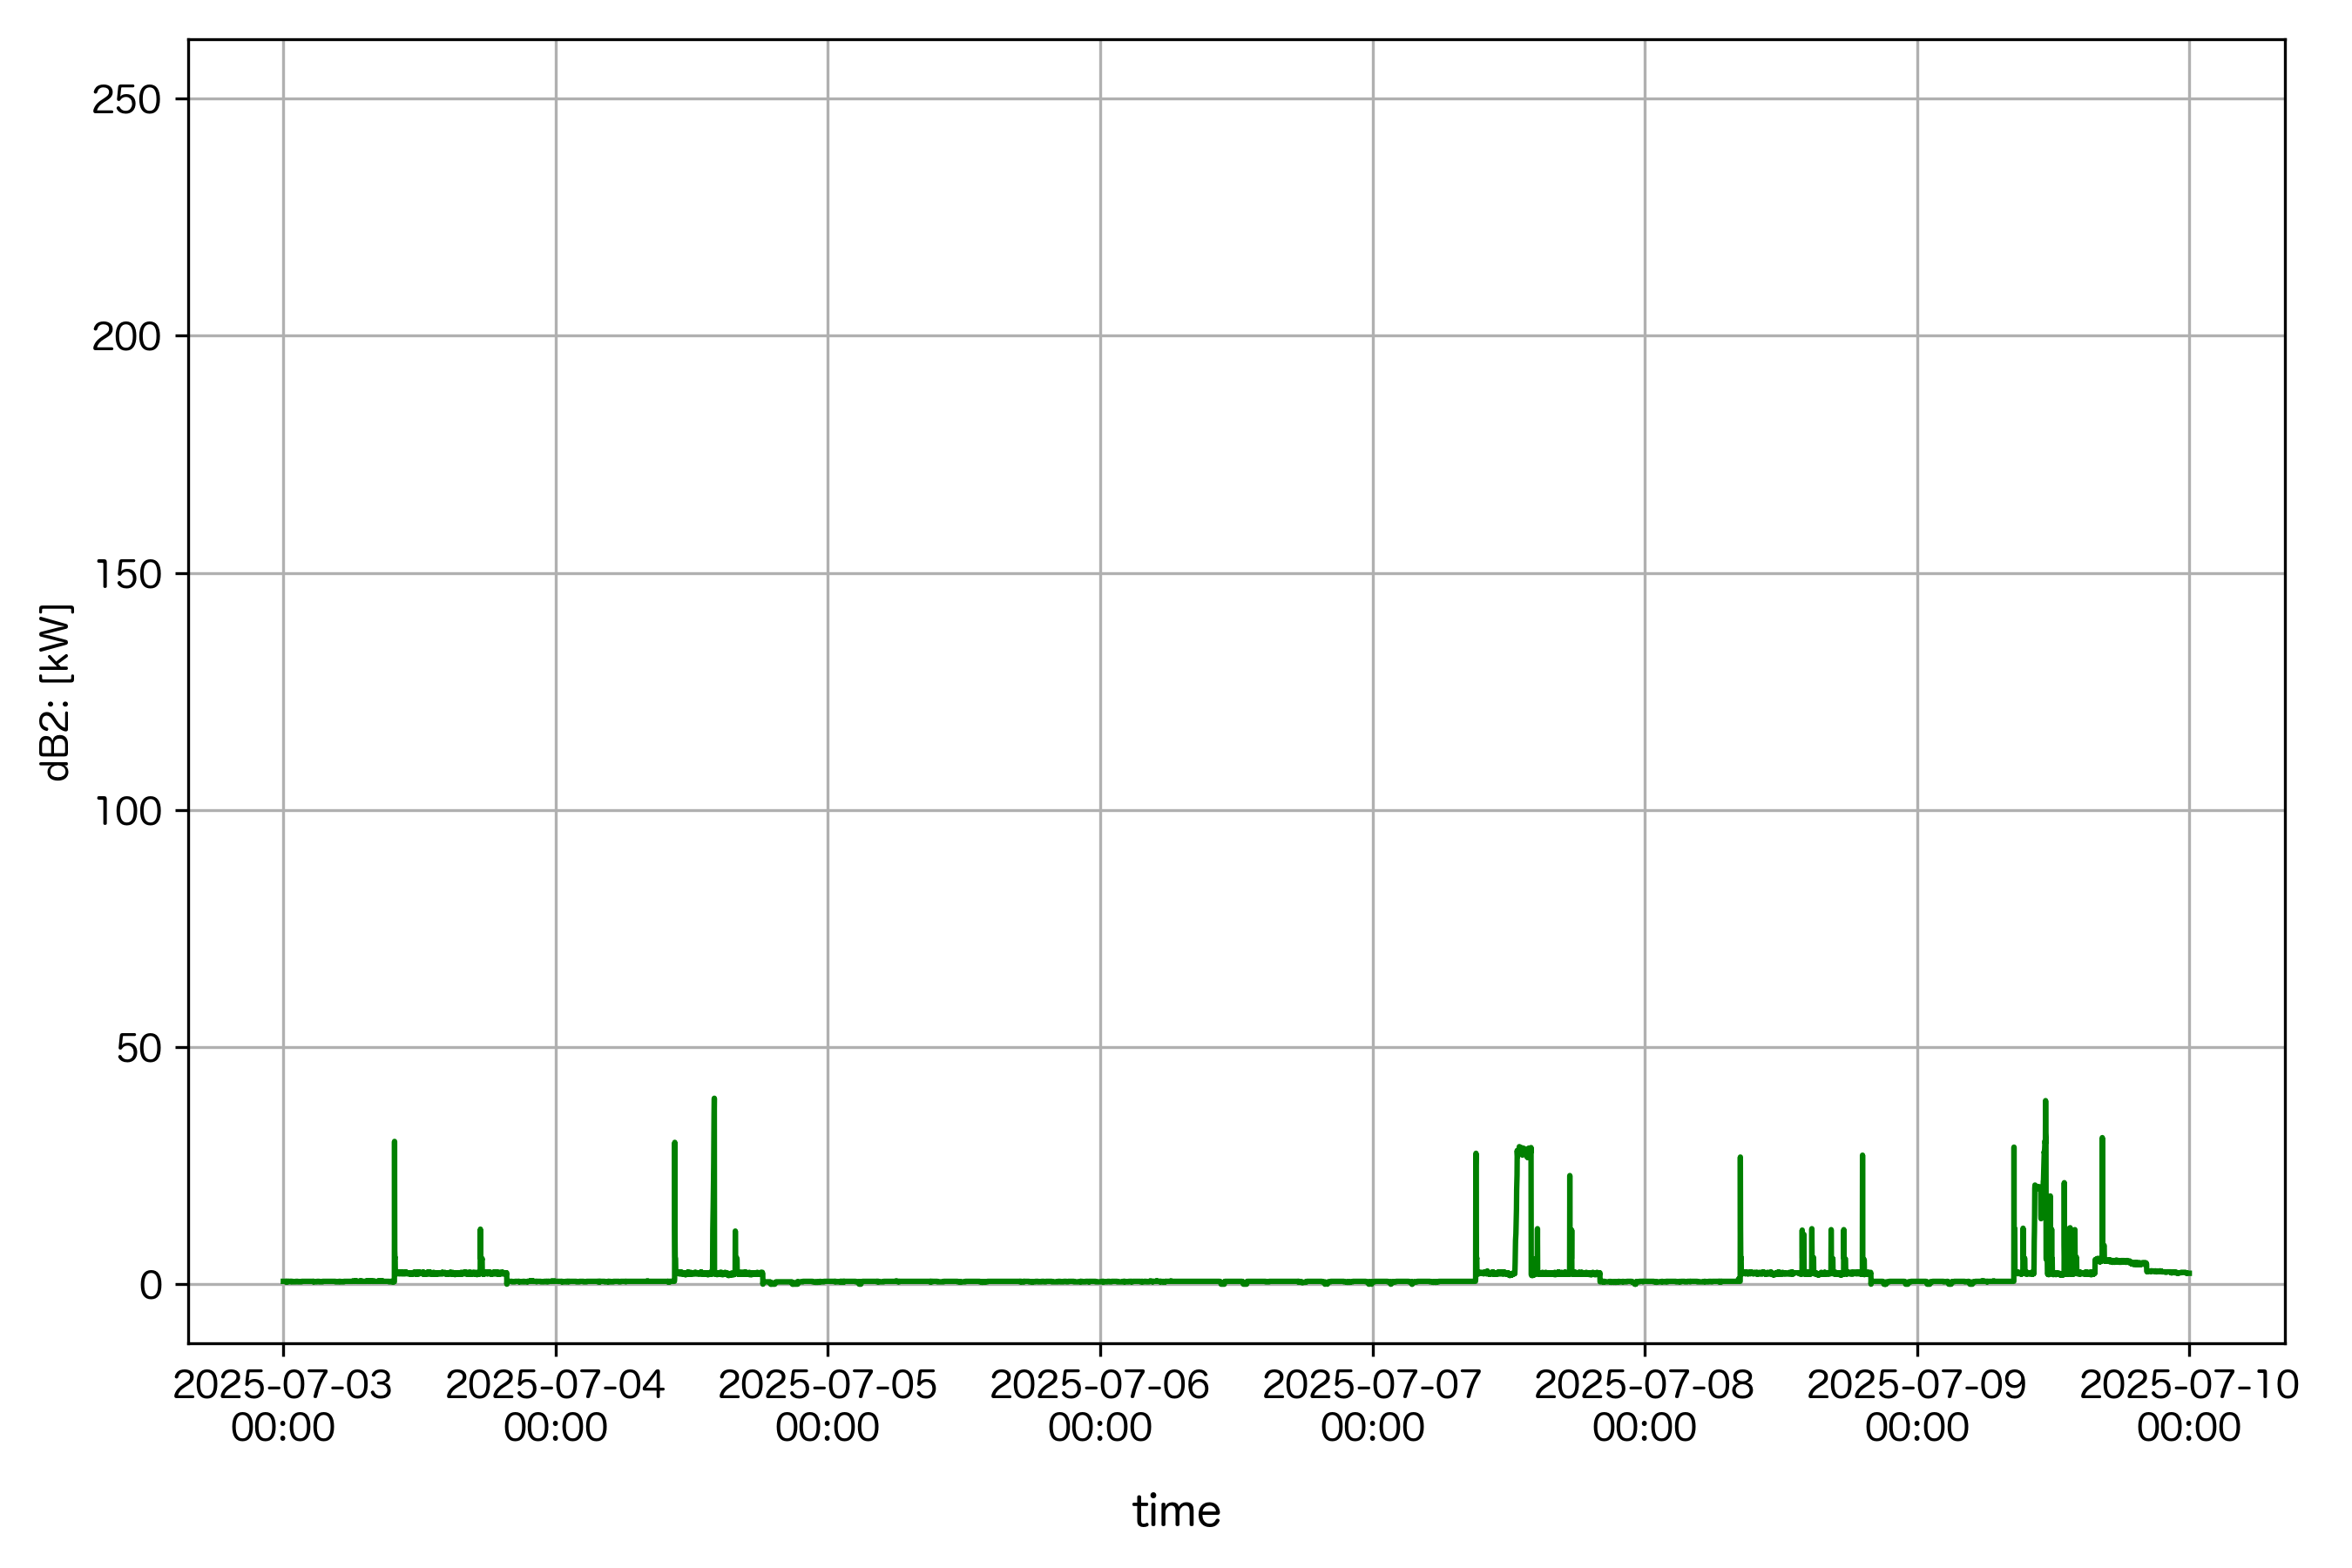
\includegraphics[width=120mm]{../figure/lp/dB2.png}
 	\caption{Power Consumption B (After Conversion)}
 	\label{fig:lp_dB2}
\end{figure}
\begin{figure}[h]
	\centering
 	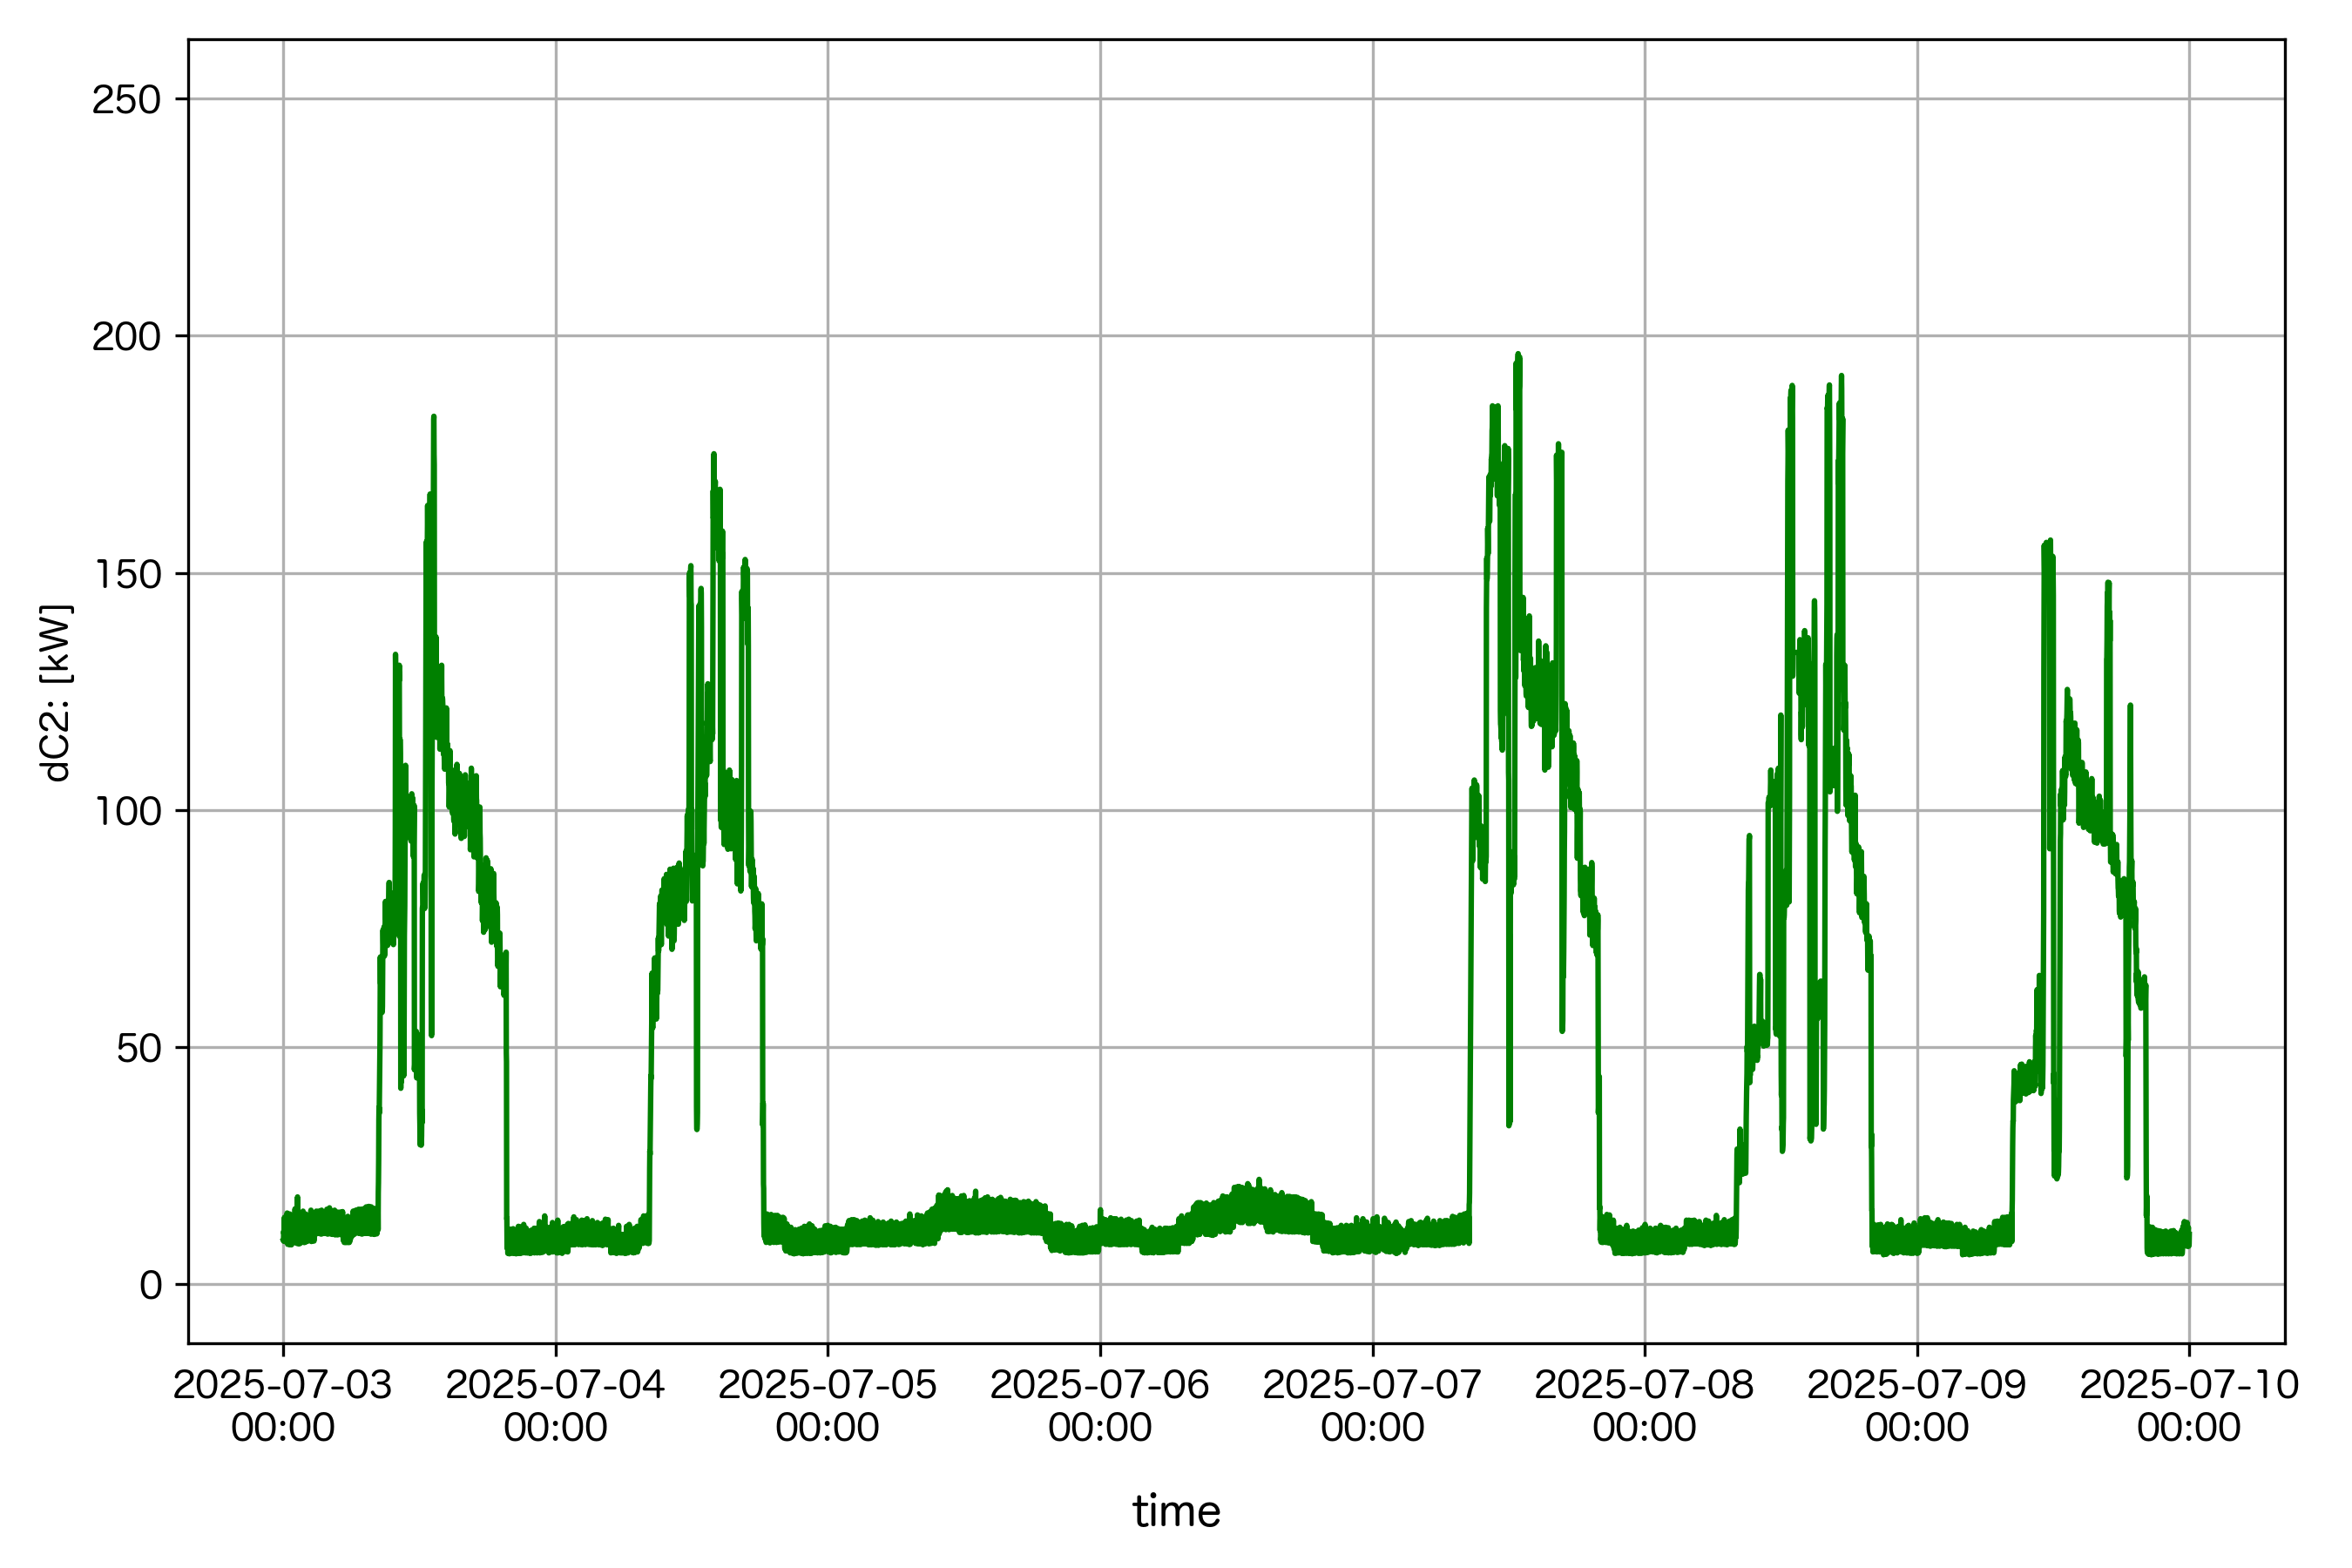
\includegraphics[width=120mm]{../figure/lp/dC2.png}
 	\caption{Power Consumption C (After Conversion)}
 	\label{fig:lp_dC2}
\end{figure}

\subsection{電力変換効率}
本研究の対象システムにおける電力変換効率を決定するため，実測データに基づく分析を行った．
図\ref{fig:efficency_g}は，電力変換器での変換前の太陽光発電量$g_k^{\rm P1}$を横軸，変換後の太陽光発電量$g_k^{\rm P2}$を縦軸にとった散布図である．

本研究では待機電力等を無視しており，変換器の物理的特性上，入力電力が0であれば出力電力も0となることから，
切片が0である一次関数で近似するのが妥当であると考えた．
最小二乗法を用いて回帰分析を行った結果，回帰直線の傾きとして$0.9449$が得られた．

本研究においては，他の電力変換器に関する詳細な入出力データが不在である．
しかしながら，一般的なパワーエレクトロニクス機器の変換効率は概ね同程度の水準にあると考えられることから，
システム全体のモデル化における代表値として上記の結果を採用し，
全ての変換効率パラメータ（$\alpha^{\rm P},\alpha^{\rm DA},\dots,\alpha^{\rm FD}$）を一律に$0.9449$と設定する．

\begin{figure}[h]
	\centering
 	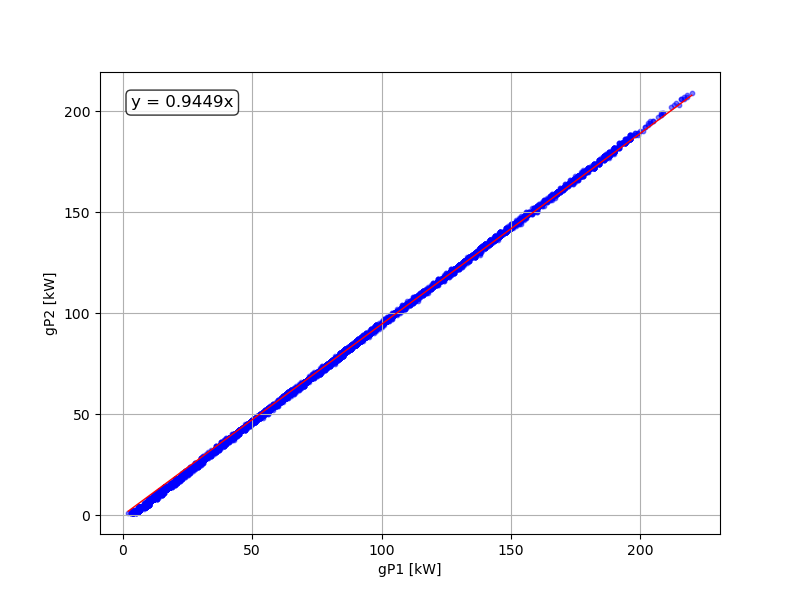
\includegraphics[width=120mm]{../figure/efficiency_g.png}
 	\caption{Correlation between input and output power in PV inverter}
 	\label{fig:efficency_g}
\end{figure}

\subsection{蓄電池}
本研究の対象に合わせ，$\overline{b}^{\rm F}$は2742 kWhとした．
なお，$b_{0}^{\rm F}$については，2025年7月3日0時00分時点における，本研究の対象の蓄電池の残量を参照し，$0.69\overline{b}^{\rm F}$ kWhとした．
また，蓄電池の最大充放電出力は450 kWであるとする．
本研究では期の刻み幅を1分としているので，$a^{\rm FC},a^{\rm FD}$は本モデルの計算ステップに合わせ$\frac{450}{60}=7.5$ kWhとした．

\subsection{商用電力系統}
1週間先までの系統電力量料金単価と系統売電単価の予測値が，1分刻みの時系列データとして与えられているものとする．
その予測値として，日本卸電力取引所（JEPX）のスポット市場における約定価格データを用いた．
JEPXの約定価格は30分単位で公開されるため，本研究では
各30分間の価格を対応する30個の期($k=30m, \dots,30m+29，m \in \{0,1,\ldots,\frac{K}{30}-1\}$）に対して一律に代入する形で入力データを作成した．
本計算例における$p_k^{\rm BY}$の値を図\ref{fig:lp_pSL}に示す．
\begin{figure}[h]
	\centering
 	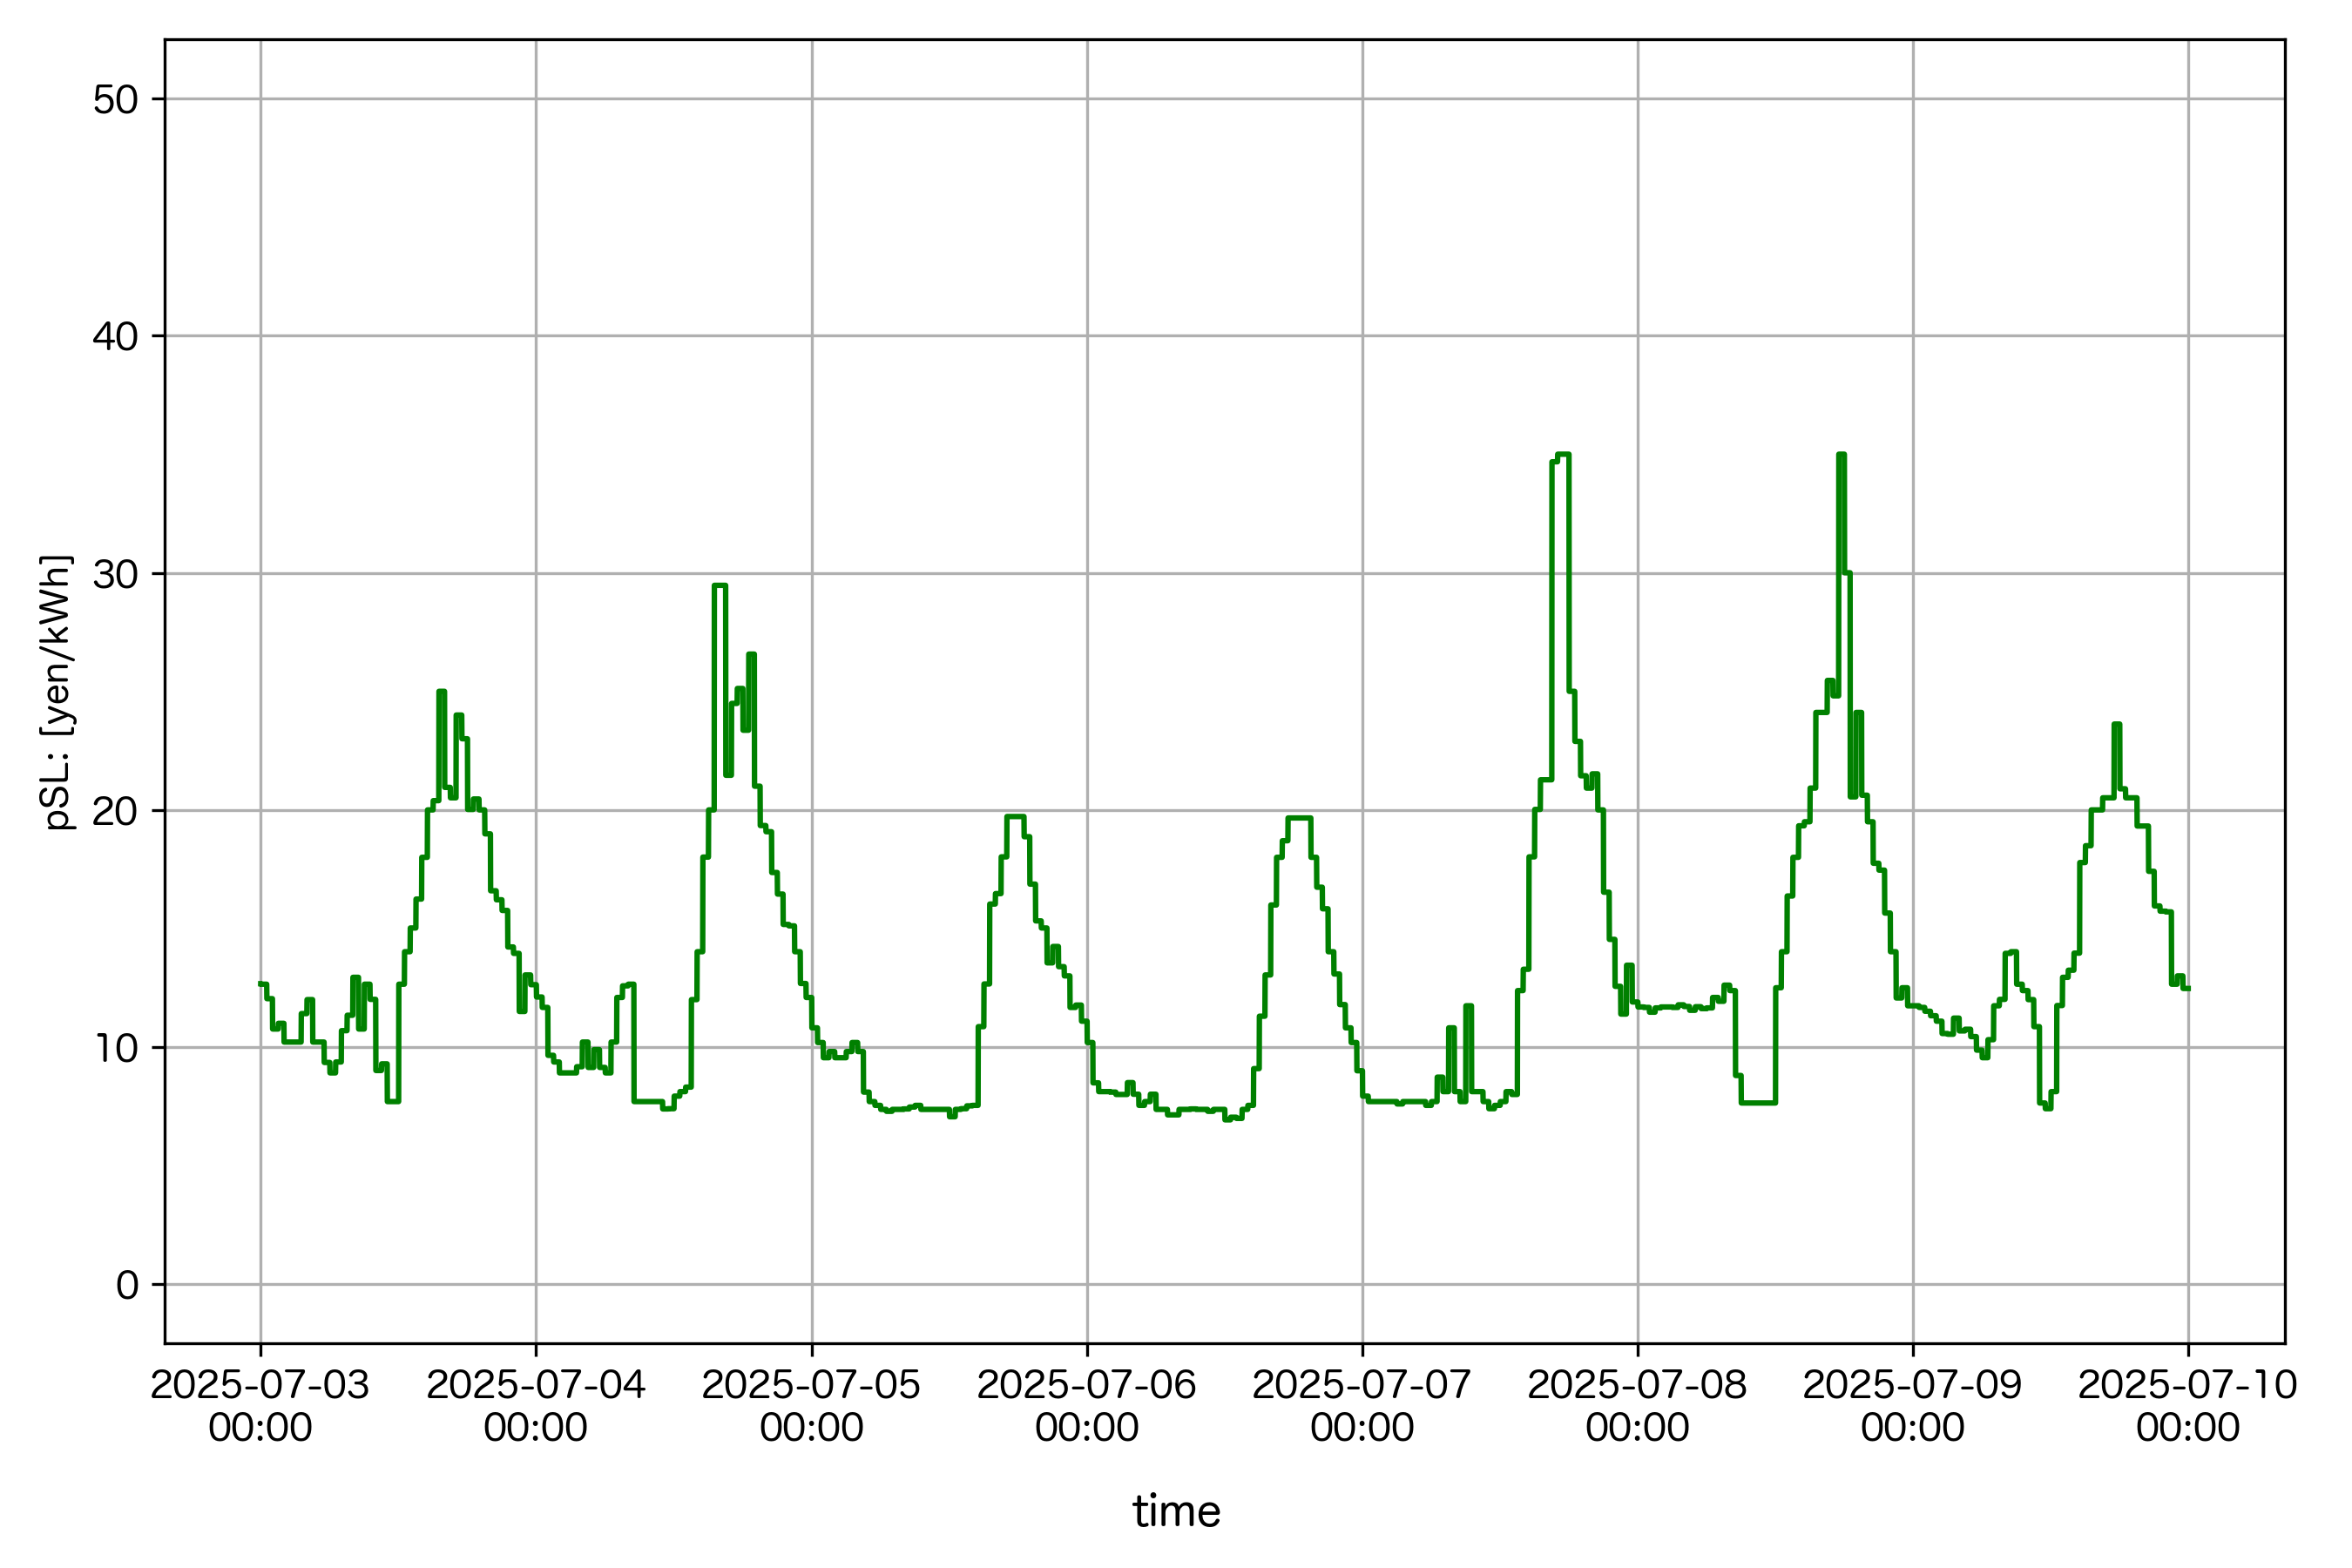
\includegraphics[width=120mm]{../figure/lp/pSL.png}
 	\caption{Electricity Purchase Unit Price}
 	\label{fig:lp_pSL}
\end{figure}

本研究で想定する市場連動型料金プランでは本来，系統買電単価と系統売電単価は同一価格となる．しかし本研究の線形計画モデルでの定式化において
$p_k^{\rm BY} = p_k^{\rm SL} $と設定した場合，同一の期に買電と売電を同時に行っても，
その収支が等しければ目的関数値に影響を与えない．その結果，最適解として同一の期に買電と売電が混在する挙動が許容される可能性がある．
このような実運用上起こり得ない現象が含まれる解を導出してしまうことを回避するために，本モデルでは系統売電単価に対して微小な負の項を導入し，
$p_k^{\rm SL}=p_k^{\rm BY} - 10^{-8}$
と定義した．こうすることにより，買電と売電を同一の期に同時に行うよりも，
いずれか一方のみを行う方が経済的に有利となる環境を数理的に構築し，同一期において買電と売電が排他的になる状態を担保することが可能となる．

また，工場からの具体的な要望として「契約電力料金の観点から，任意の連続する30分間の区間について，商用電力系統からの総買電力を 50 kW 以下に制限すること」という制約があったと仮定する．
よって，$a^{\rm BY}$は$\frac{50}{2}=25$ kWhとなる．
ところが，この制約を動的計画法の問題に反映させようとすると，
 異なる期同士が影響し合うため，過去の買電量の履歴を保持する必要があり，状態空間の増大を招くことになる．
 そのため，議論を単純にするために，この制約を元の制約より緩い制約にならないように気をつけながらより簡単な制約にしなければならない．
そこで，動的計画モデルの本計算例では「すべての期について商用電力系統から買う電力量が$\frac{50}{60}$ kWh以下でなければならない」という，期をまたがないような制約に改めた．


\section{動的計画モデルにおける，時間的計算量に関連する定数の設定}
本問題の求解にかかる時間的計算量は，更新式に則って評価値を更新する部分がボトルネックとなり，$O(B\{ \frac{(B-1)(\Delta s_k^{\mathrm{Max}}(s_{k-1}) - \Delta s_k^{\mathrm{Min}}(s_{k-1}) )}{\overline{b}} +1\} K)$となる．$\frac{\overline{b}}{B-1}$は残量の隣り合う段階の間隔であるから，
 $\frac{(B-1)(\Delta s_k^{\mathrm{Max}}(s_{k-1}) - \Delta s_k^{\mathrm{Min}}(s_{k-1}) )}{\overline{b}} +1$はある状態$s_k$について高々遷移可能な状態遷移の数を表す．
 
$K$については1週間についての運用計画を考えることが決まっていることから値を自由に変更することができない．
また，$\Delta s_k^{\mathrm{Max}}(s_{k-1})$は蓄電池の最大放電量に依存し，$\Delta s_k^{\mathrm{Min}}(s_{k-1}) $は蓄電池の最大充電量と系統からの最大買電量のうちの大きくない方に依存する値であるため，値を自由に設定することはできない．
十分高速に解を得るためには，$B$の値をどの程度の大きさに設定するのかを
考える必要がある． 

$B$に関連する制約として，「すべての期について商用電力系統から買う電力量が$\frac{50}{60}$ kWh以下でなければならない」という制約がある．
この制約をもとに$B$の値を決定することを考えるが，まず，$B$の値が小さすぎる場合，
 買電を行う状態遷移のうち，系統から買う電力量が$\frac{50}{60}$ kWh以下になるようなものが存在しなくなってしまい，
 実質的に「買電をしてはいけない」という制約になってしまう．また，残量の隣り合う段階の間隔が大きくなるため誤差が大きくなってしまうというデメリットも伴う．
 逆に，$B$の値が大きすぎる場合，遷移可能な状態遷移が多くなりすぎてしまい求解に時間を要することになる．これらを考慮して，残量の隣り合う段階の間隔が$0.2$ kWh，
 すなわち，12 kW刻みの電力となるように$B$を設定した．
蓄電池容量は$\overline{b}=2742$ kWhであるため，このとき$B$の値は13710となる．この$B$の値であれば各々の状態について，
買電を行う状態遷移が少なくとも4つ現れることになり，時間的計算量を抑えつつも，実用上十分な粒度で状態遷移を表現できる．

\section{線形計画モデルによる計算結果}
線形計画モデルでの計算結果を以下に示す．
まず，全期間の系統買電力を図\ref{fig:lp_sBY_sSL}に示す．
なお，図中の負の値は商用電力系統への売電を表している．
図\ref{fig:lp_sBY_sSL}より，7月6日を除くの6日間について，各日の午後の短い期間に集中して売電を行っていることが確認できる．
ここで，同時期の系統売電単価（図\ref{fig:lp_pSL}）を参照すると，
売電単価が高騰する期と売電の期が一致している．
このことから，本モデルは売電収益を最大化するために，単価が高い時間帯を的確に捉えた運用を実現しているといえる．

次に，全期間の系統買電力のうち特に7月3日の0時00分から11時59分までの12時間分の結果を図\ref{fig:lp_sBY_sSL_first_12h}に示す．
図\ref{fig:lp_sBY_sSL}では50 kWを超える買電が散見されるが，これは本モデルの制約が「30分間の平均電力」を対象としていることに起因すると考えられる．
具体的に図\ref{fig:lp_sBY_sSL_first_12h}を観察すると，大量に買電を行う期間と，買電を極力抑える期間が周期的に現れている．
これは，30分という時間枠の中で瞬時的に電力を購入しつつ，枠内の残りの時間で調整を行うことで，
30分平均の最大需要電力を規定値以下に抑制しようとする挙動である．
ここで，30分間の枠内では売電単価が一定であるにもかかわらず，特定の期に買電が集中している．
この要因として，式\eqref{eq:b_f}における蓄電池の自己放電が関連していると考えられる．
蓄電池は残量に比例してわずかな目減りが発生するため，モデルは損失を最小化しようと働く．
すなわち，売電を行う直前まで蓄電池の残量を低く維持し，売電の直前で集中的に買電を行うことで，蓄電期間中のエネルギー損失を抑制する運用が選択されたと考えられる．

最後に，期ごとの蓄電池残量の推移を図\ref{fig:lp_bF}に示す．図より，最終期に蓄電池の残量が0となっていることがわかる．
これは，目的関数値を最小化するために，溜まっている蓄電池の電力を全て使い切る形で売電してしまおうとしているためである．
しかし，実世界での運用は$K$期以降も連続的に継続するものである． 
したがって，実用化に際しては，翌期以降の電力需要を考慮し，期間終了時の蓄電残量に一定の下限値を設けるなどの対応が必要であると考えられる．
\begin{figure}[h]
	\centering
 	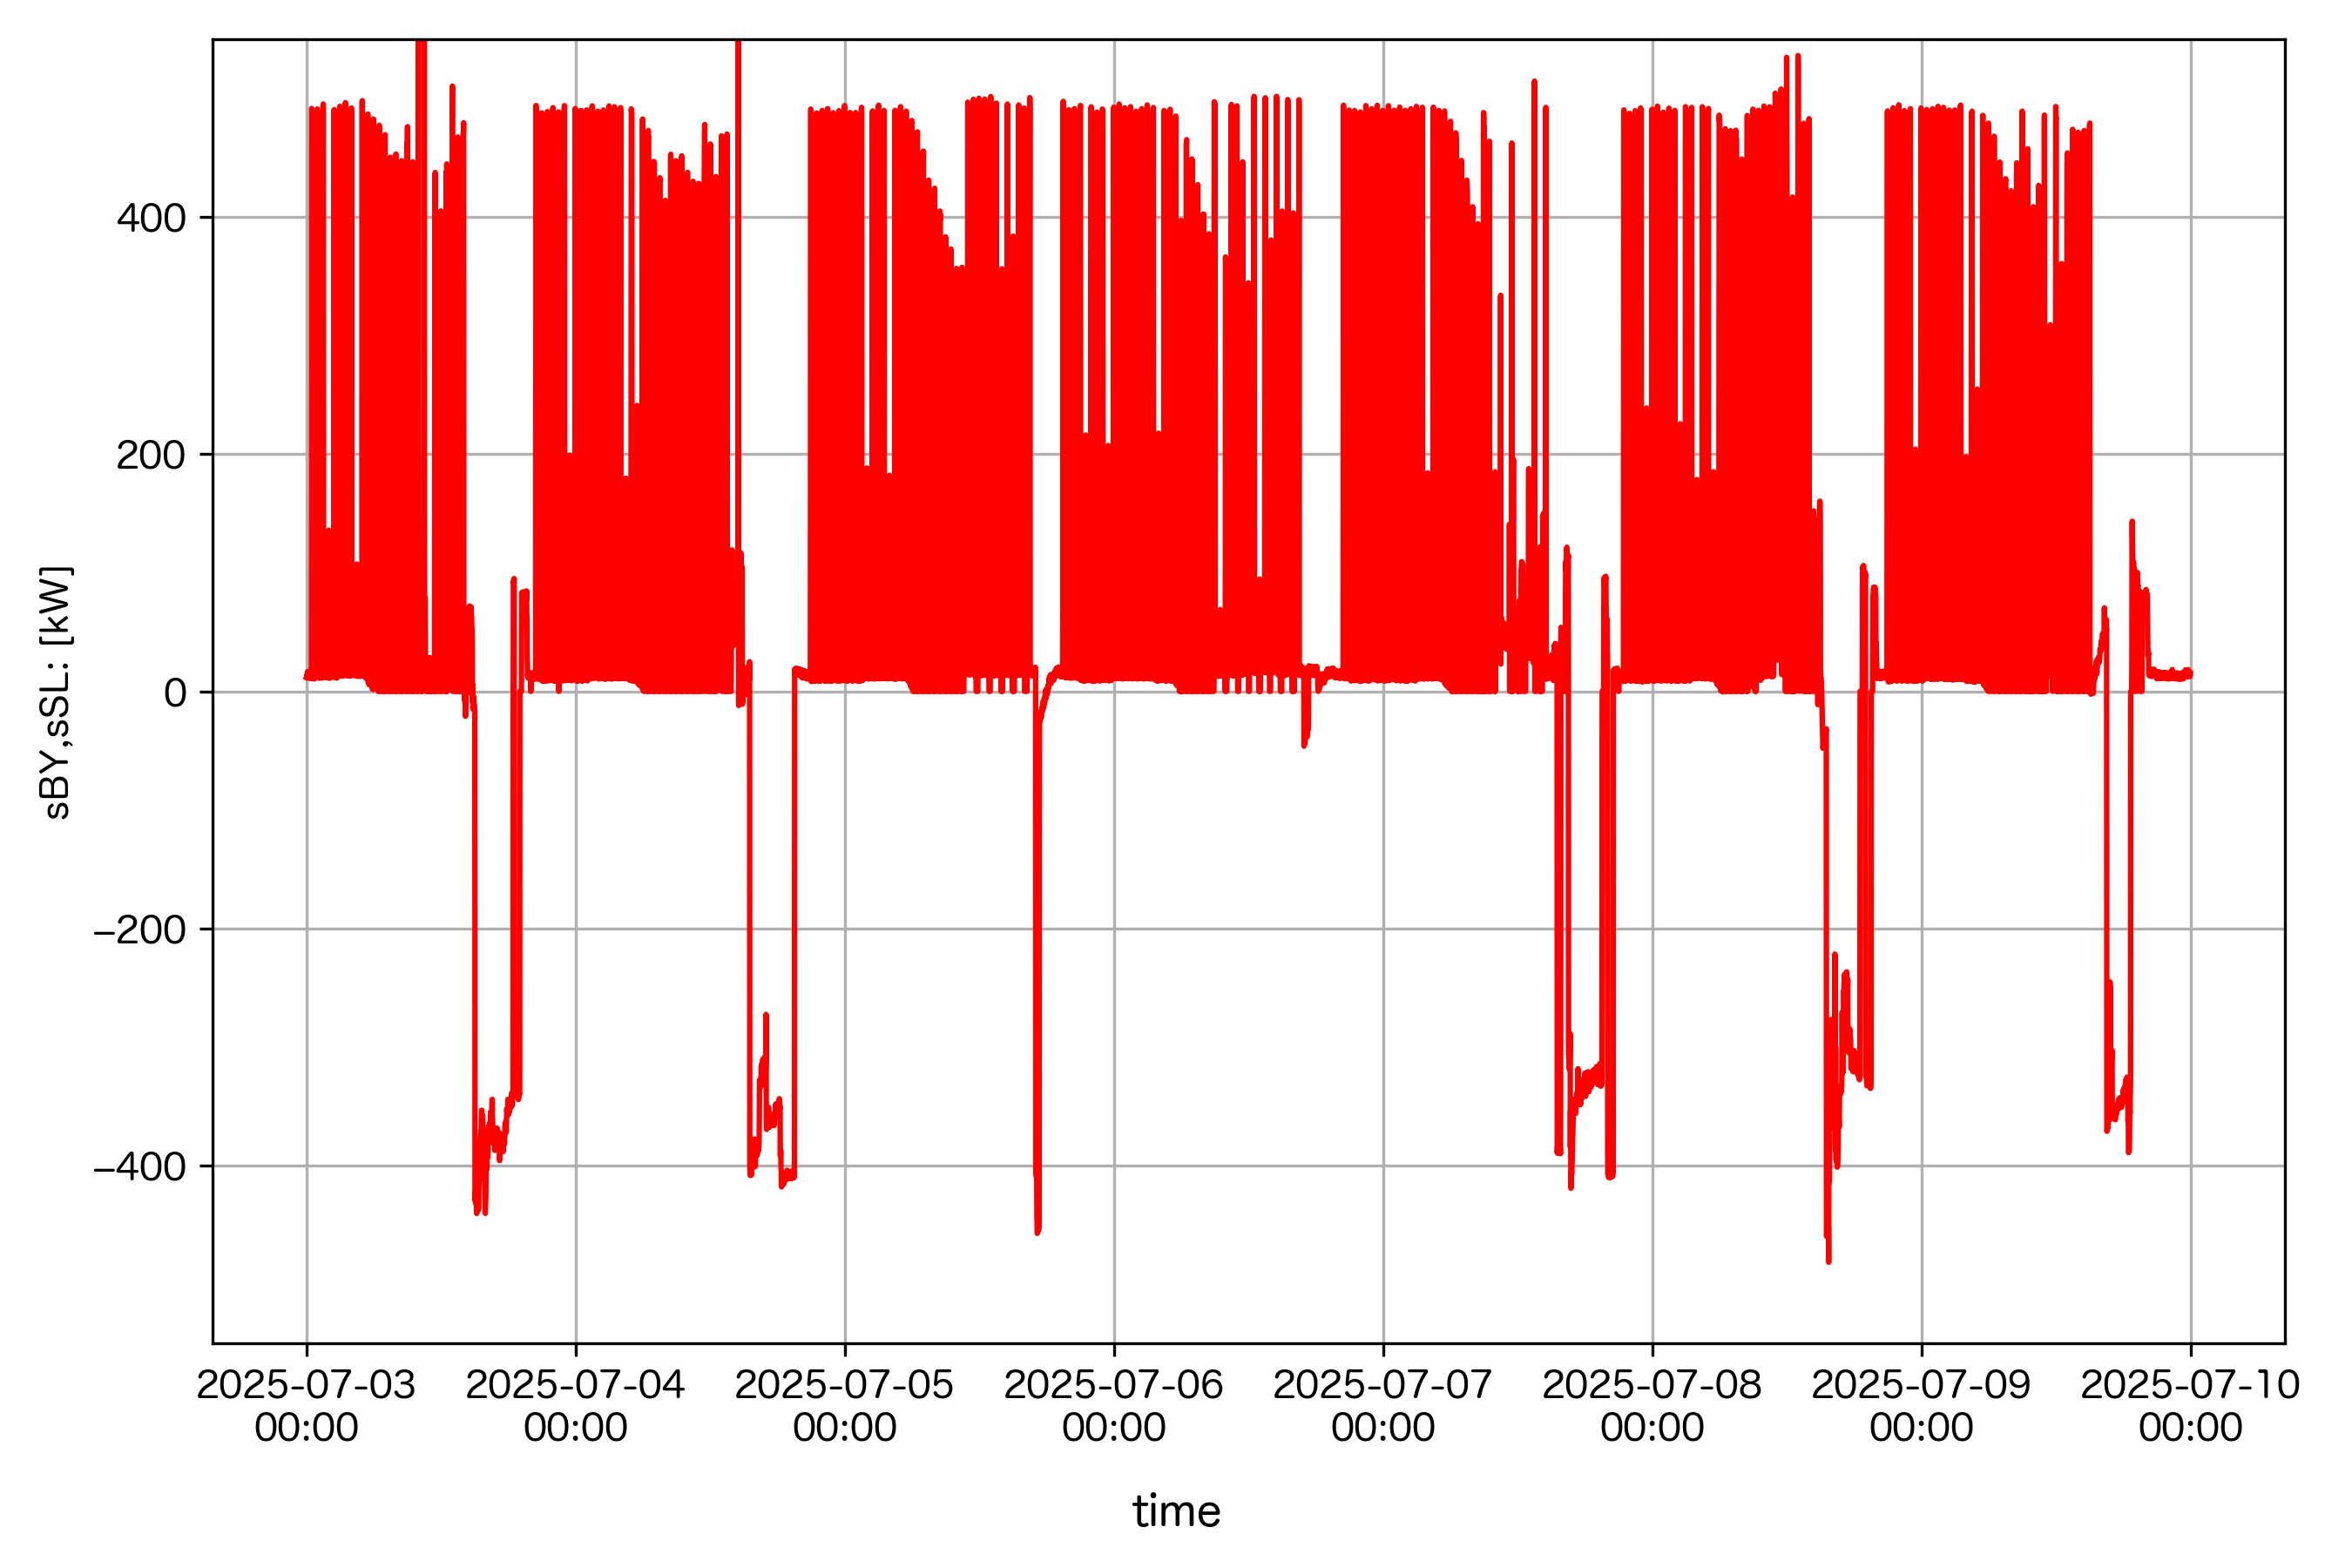
\includegraphics[width=120mm]{../figure/lp/sBY_sSL.png}
 	\caption{Grid Power Purchase}
 	\label{fig:lp_sBY_sSL}
\end{figure}

\begin{figure}[h]
	\centering
 	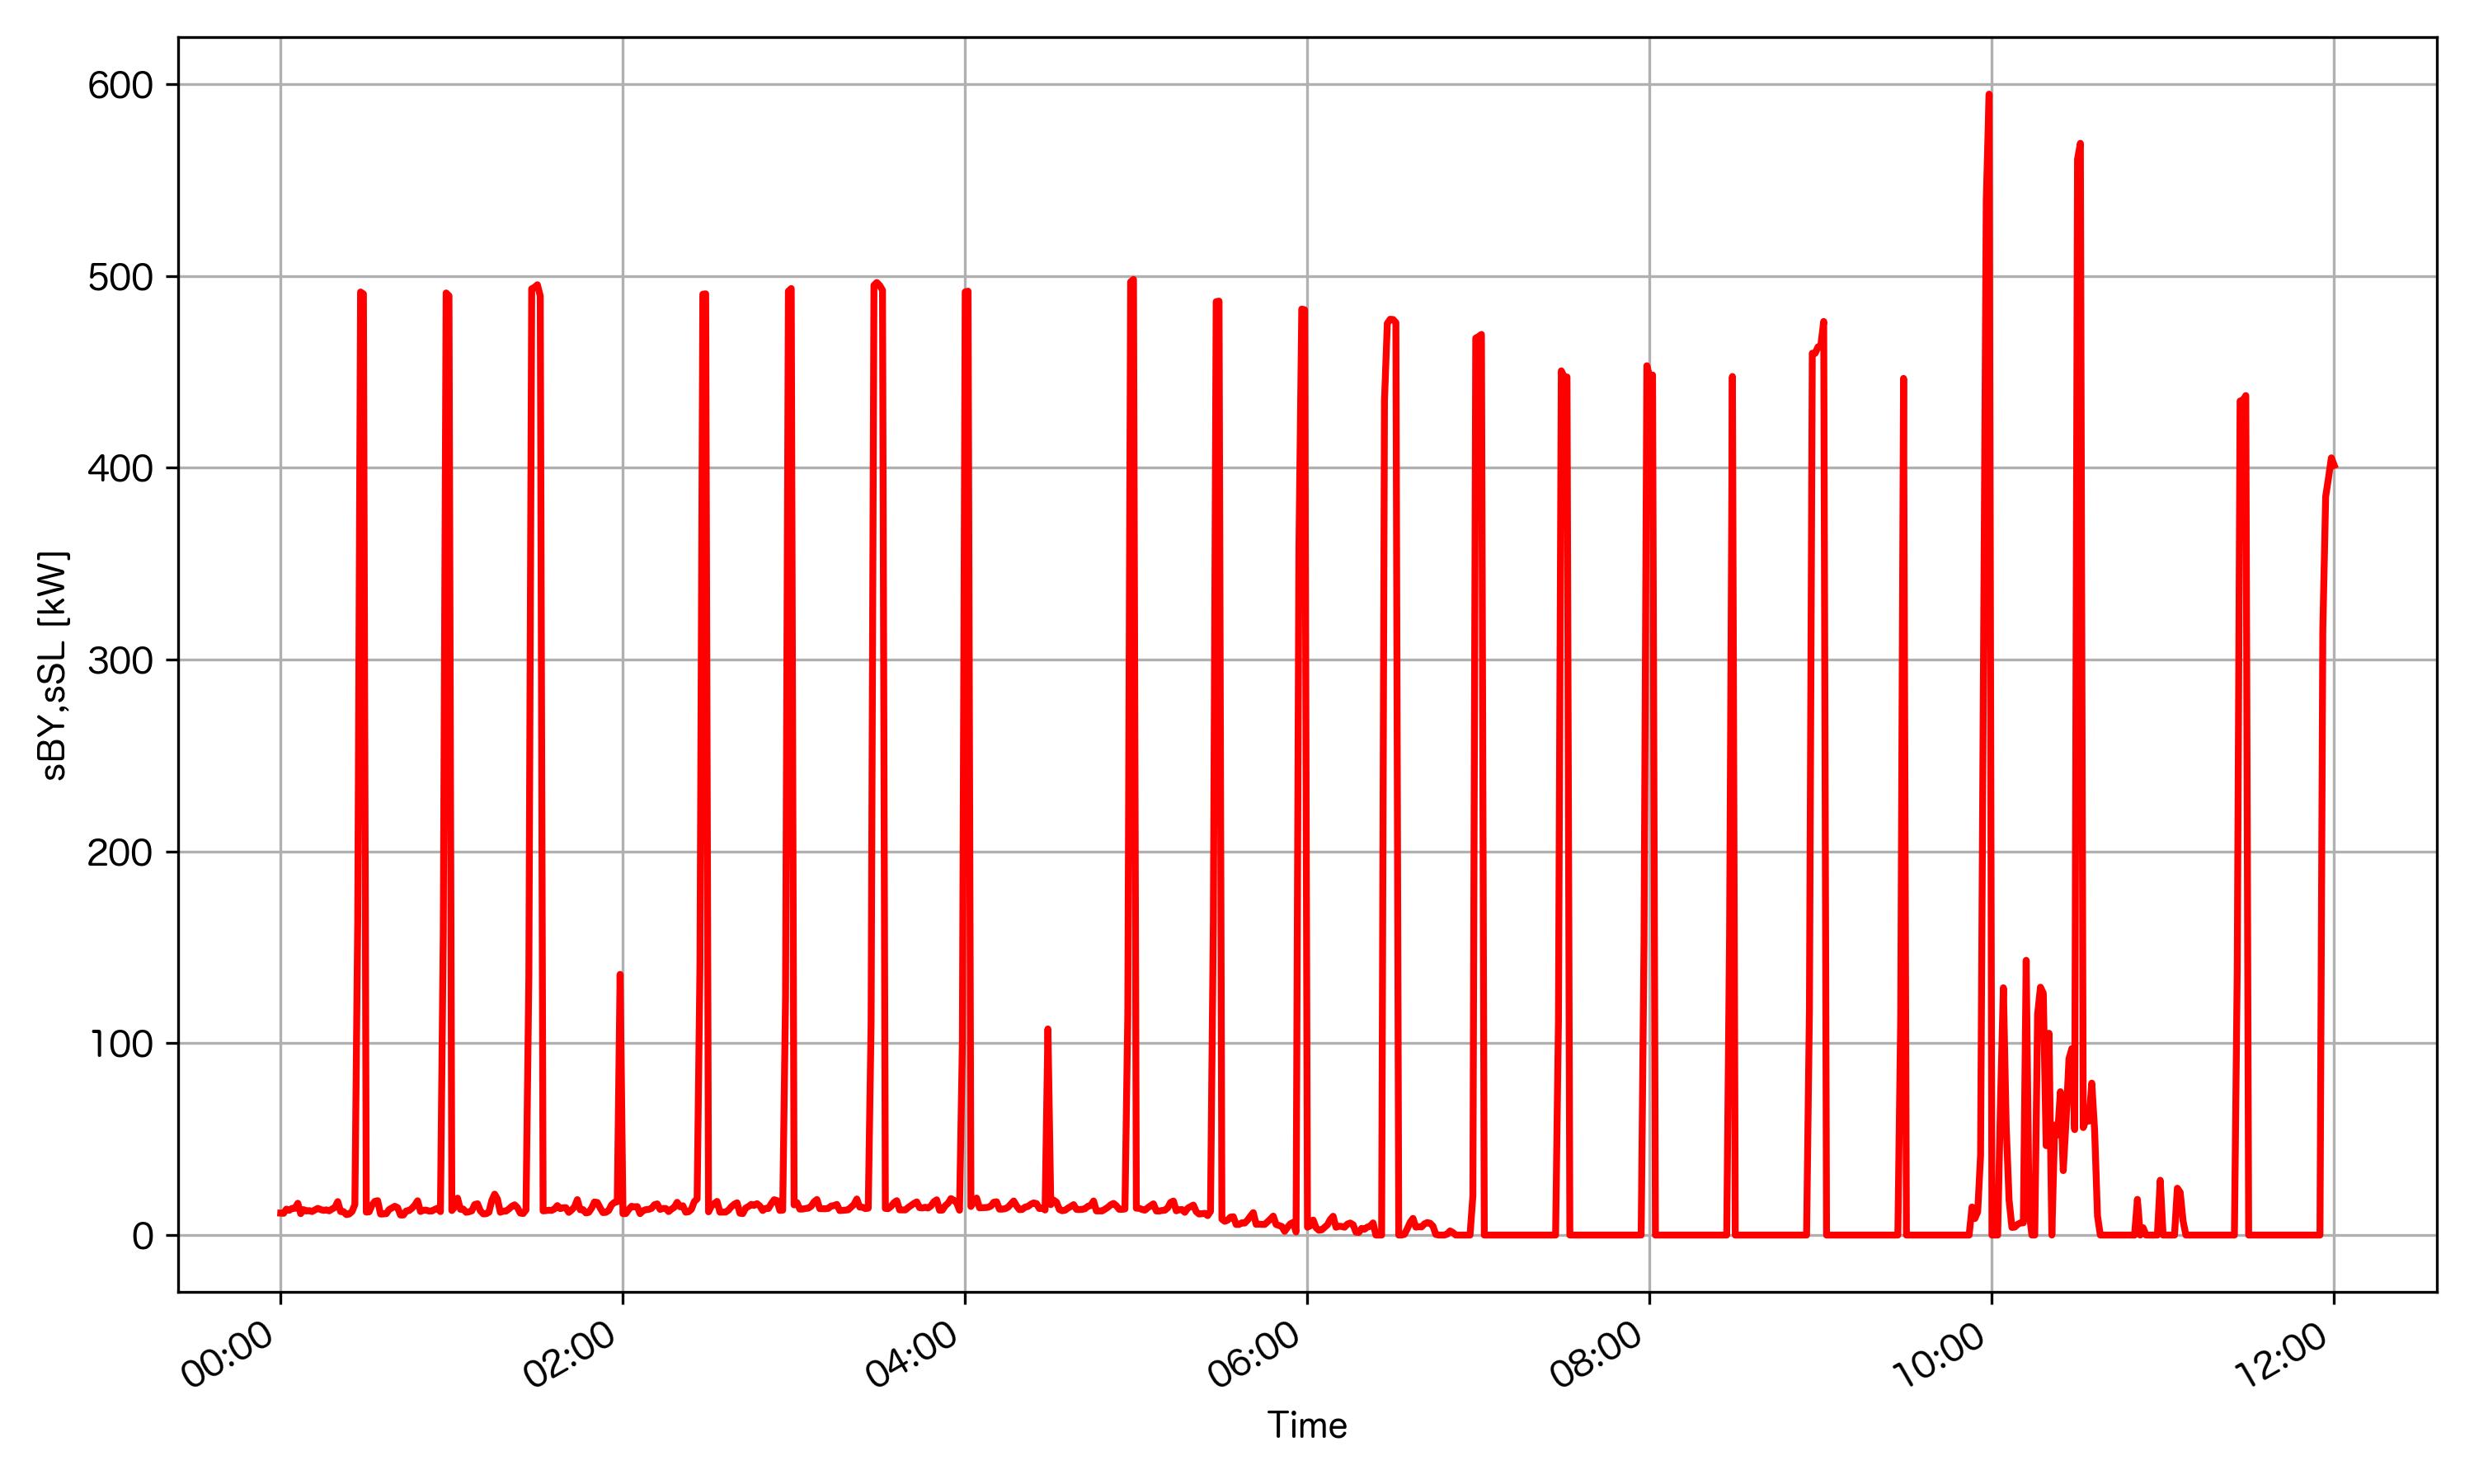
\includegraphics[width=120mm]{../figure/lp/sBY_sSL_first_12h.png}
 	\caption{Grid Power Purchase(First 12 Hours)}
 	\label{fig:lp_sBY_sSL_first_12h}
\end{figure}

\begin{figure}[h]
	\centering
 	
\includegraphics[width=120mm]{../figure/lp/bF.png}
 	\caption{Battery State of Charge}
 	\label{fig:lp_bF}
\end{figure}

\section{動的計画モデルによる計算結果}
同様の問題を動的計画モデルで解いたものを図\ref{fig:dp_sBY_sSL}，\ref{fig:dp_bF}に示す．
計算結果を確認すると，線形計画モデルと同様の期で，瞬間的に売電を行っており，
最終期の末に蓄電池の容量を使い果たすように蓄電池の電力を使用していることがわかる．
また，線形計画モデルとの顕著な相違点として，系統からの買電量が50 kWを超えている期が存在しない点が挙げられる．
線形計画モデルでは「任意の連続する30分間の区間について，商用電力系統からの総買電力を 50 kW 以下に制限すること」という制約を採用しているため，
 30分枠内で瞬間的に50 kWを超過する挙動が許容されていた．
一方，動的計画モデルにおいて同様の制約を課すためには，過去の買電量の履歴を保持する必要があり，状態空間の増大を招く．
そのため本モデルでは，状態空間の次元を抑えるために，本来30分間での制約であるものを，
1分あたりの買電力量が $\frac{50}{60}$ kWh以下であるという，より厳しい制約に置き換えて適用している．
図\ref{fig:dp_sBY_sSL}において買電量のピークが低く抑えられているのは，この制約条件の違いによるものである．
しかしながら，図\ref{fig:dp_bF}に示す蓄電池残量の推移は線形計画モデルの結果と概ね一致している．

\begin{figure}[h]
	\centering
 	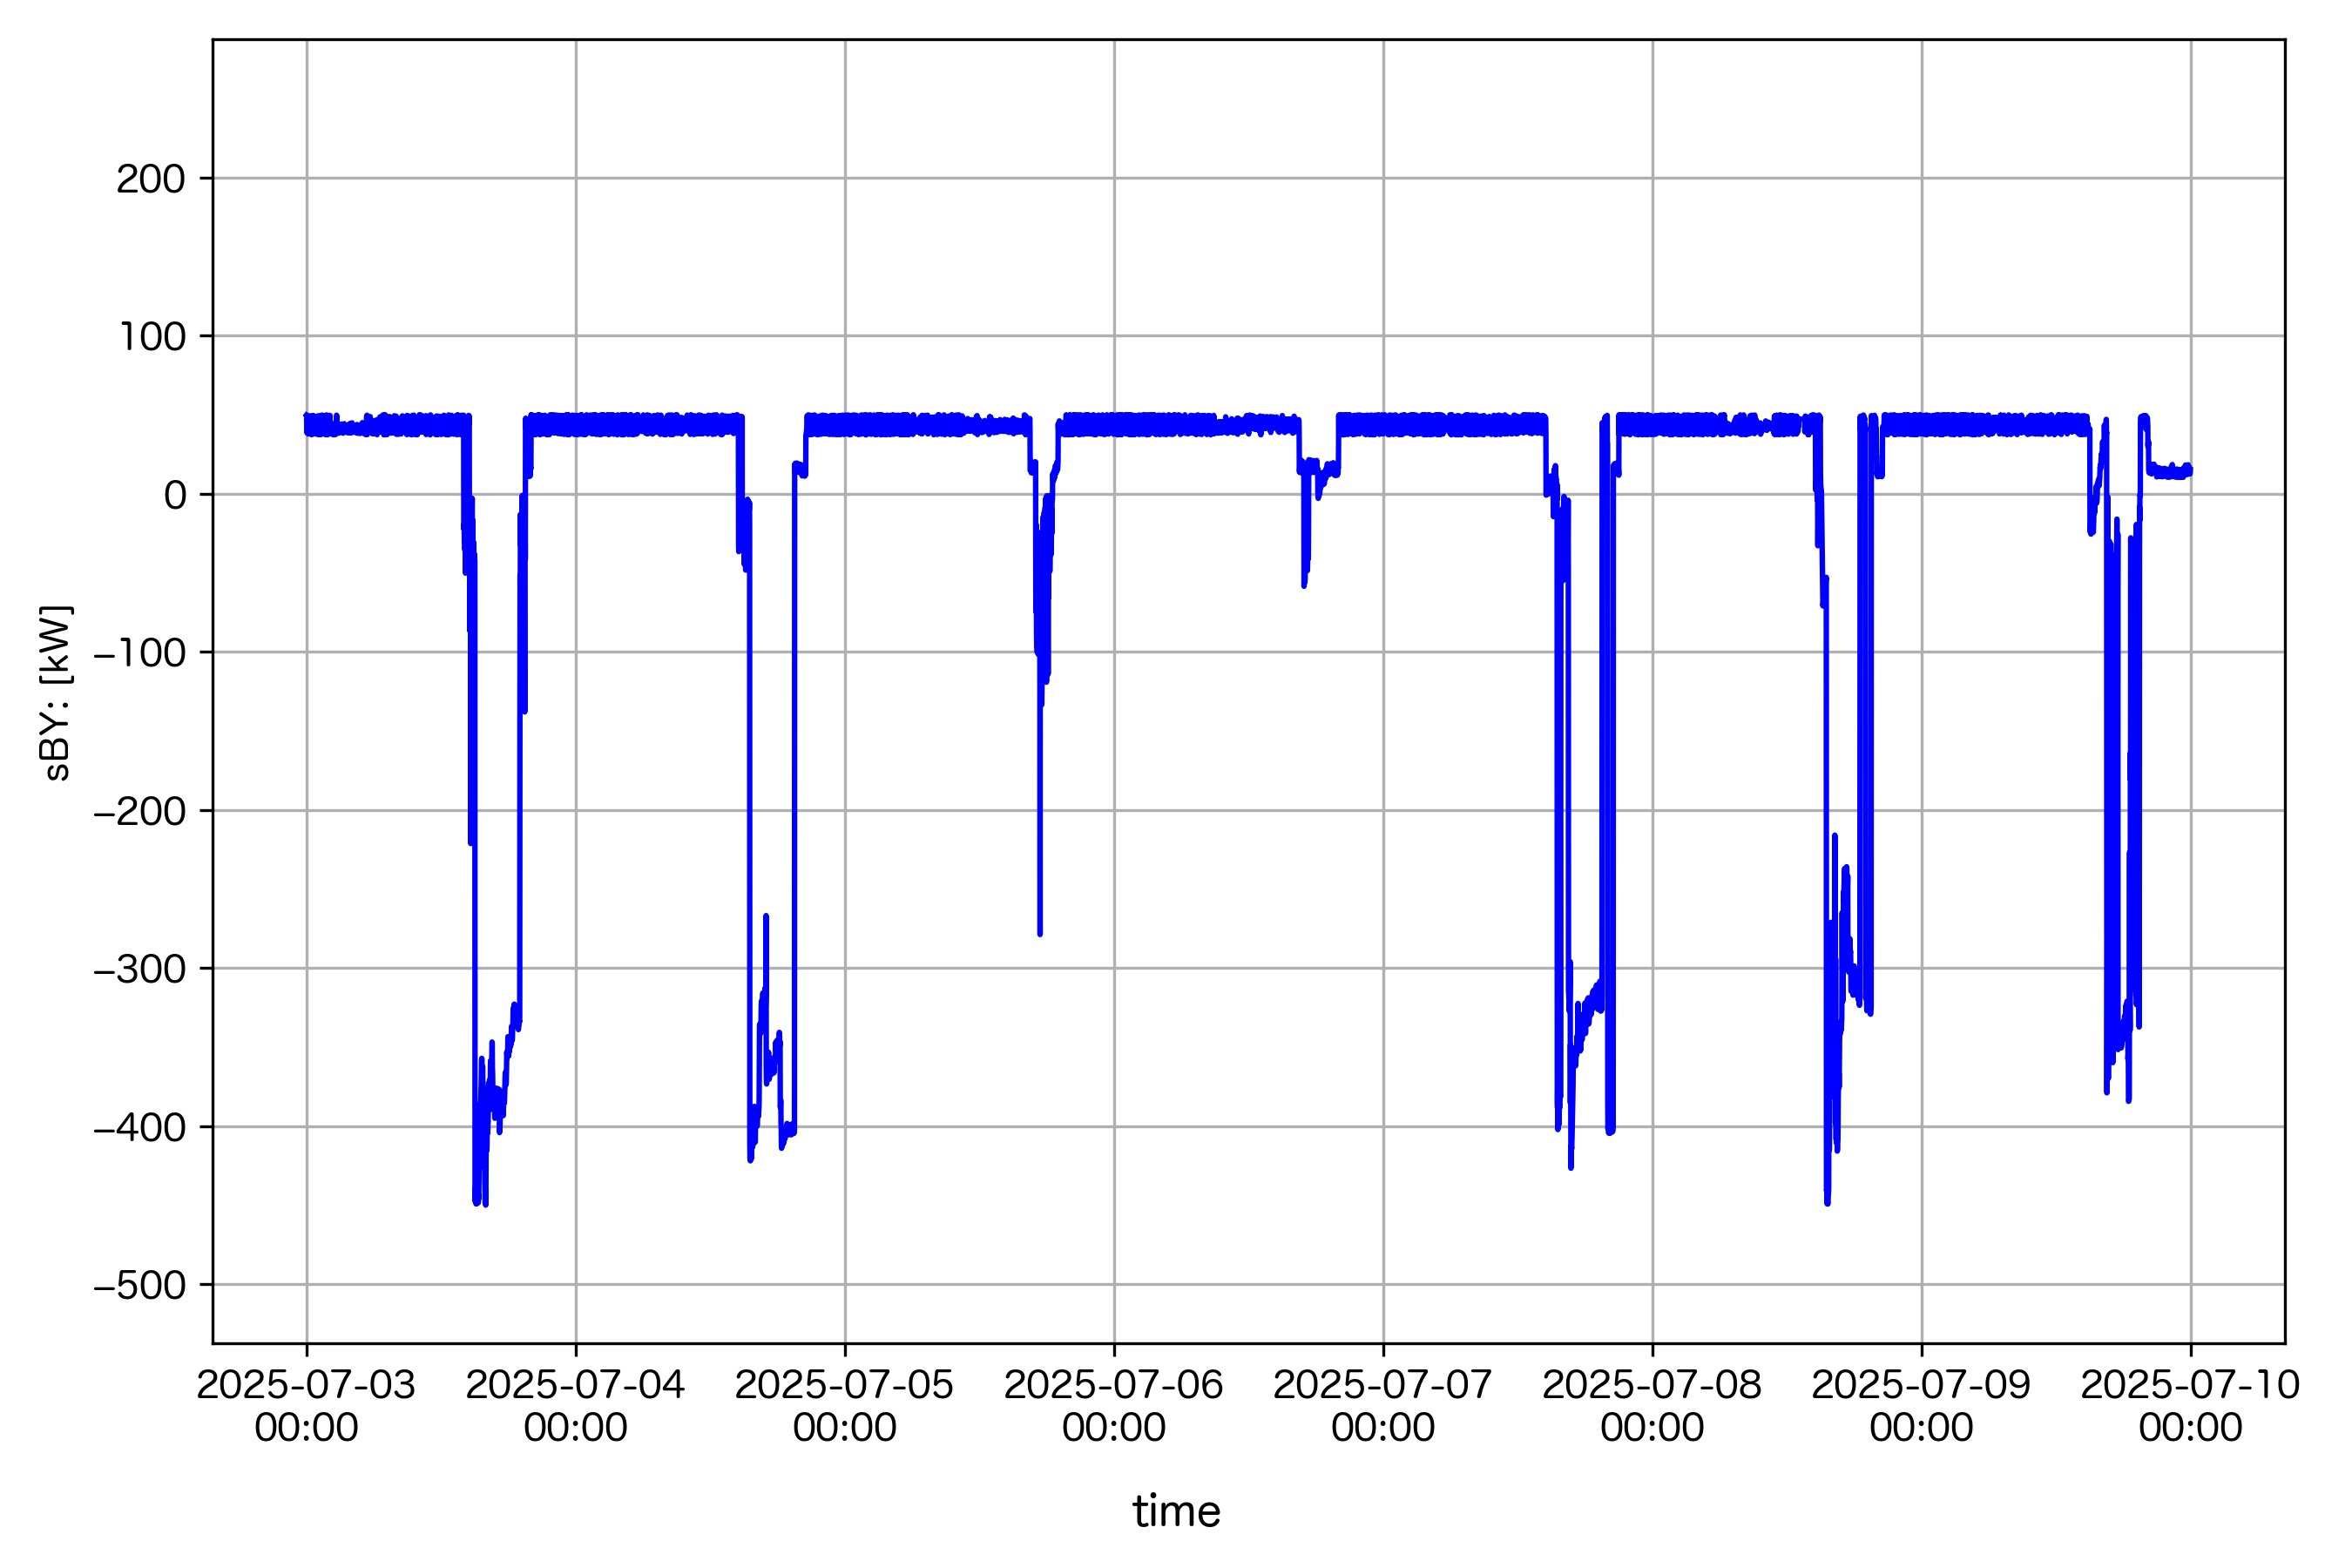
\includegraphics[width=120mm]{../figure/dp/sBY.png}
 	\caption{Grid Power Purchase}
 	\label{fig:dp_sBY_sSL}
\end{figure}

\begin{figure}[h]
	\centering
 	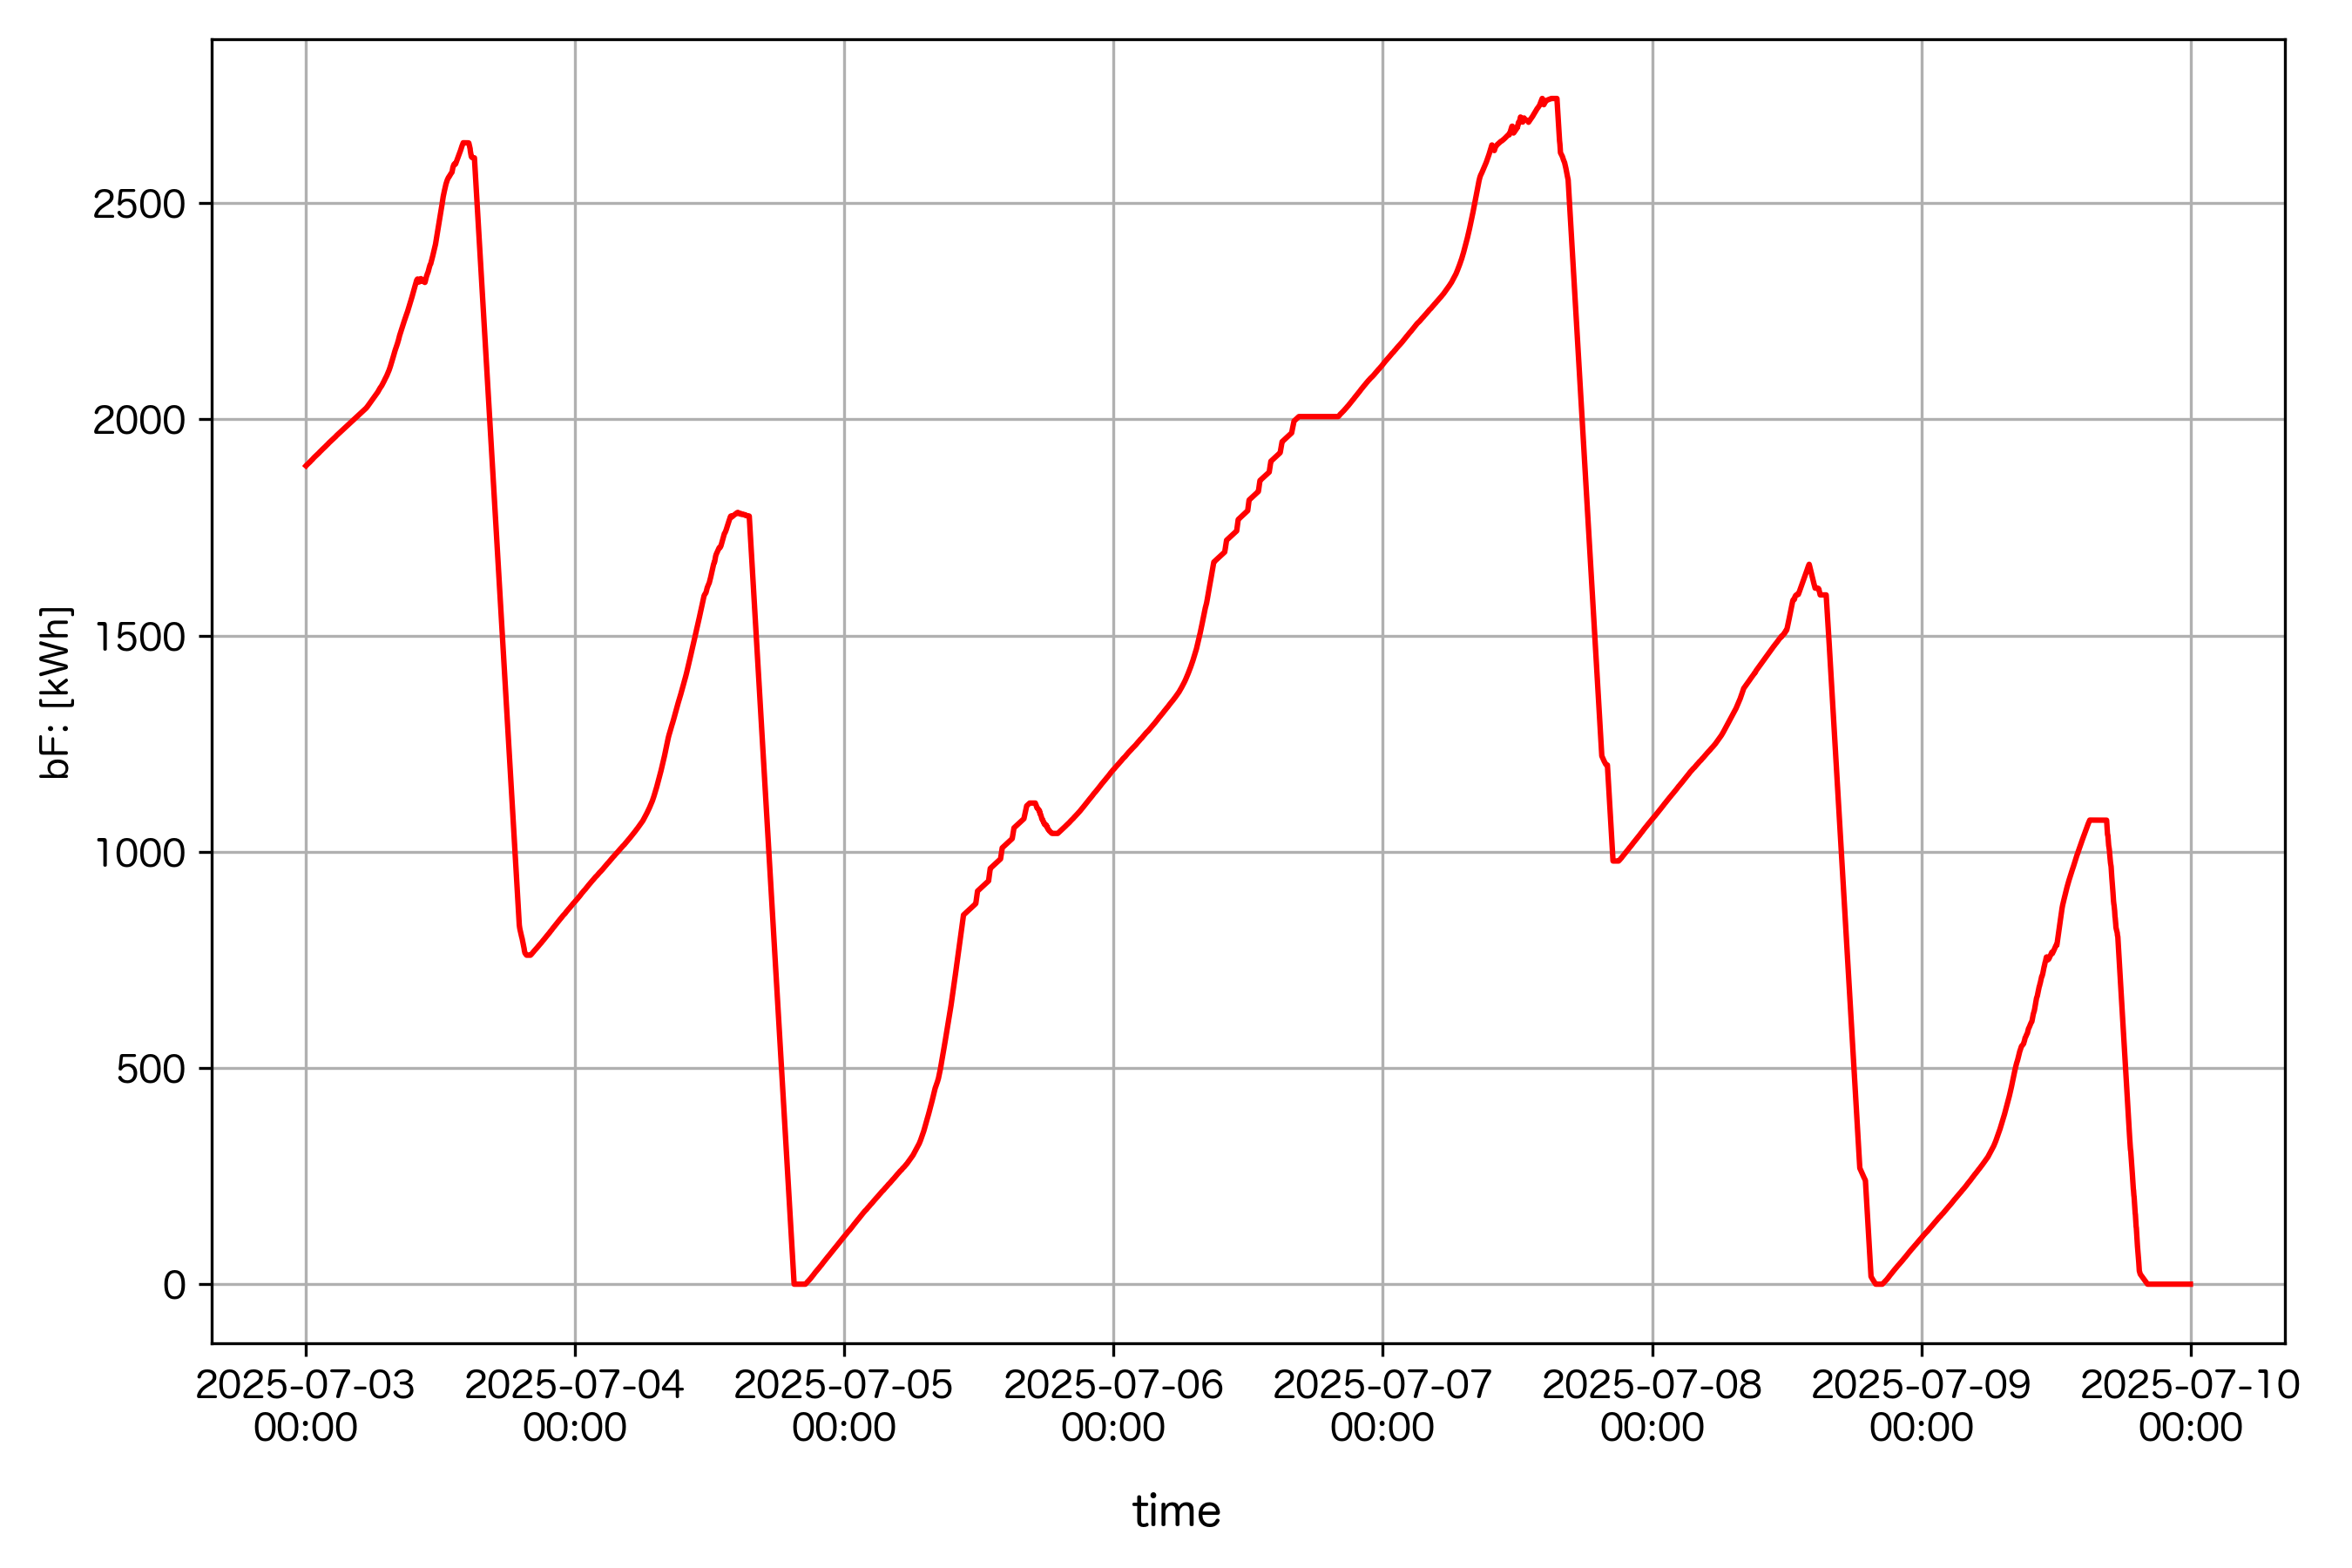
\includegraphics[width=120mm]{../figure/dp/bF.png}
 	\caption{Battery State of Charge}
 	\label{fig:dp_bF}
\end{figure}

\section{線形計画モデルと動的計画モデルの目的関数値の比較}
本節では，両モデルによって導出された最適目的関数値を比較し，動的計画モデルの解の質について評価を行う．
また，動的計画モデルにおける蓄電池残量の分割数$B$が解の精度に与える影響についても検証する．
表\ref{table:objective_comparison}に，各モデルにおける最適目的関数値を示す．
ここで，動的計画モデルについては，分割数$B$を本例題と同様である10080と，本例題の2倍とした20160，および本例題の1/2倍とした5040の
3つのケースにおける結果を示した．
なお，目的関数値は正味の支出を表しており負の値は利益，すなわち，売電収益が買電コストを上回った状態を意味する．

\begin{table}[htbp]
  \centering
  \caption{Comparison of Optimal Objective Function Values}
  \label{table:objective_comparison}
  \begin{tabular}{lcc}
    \hline
    Model & Objective Value\\
    \hline \hline
    Linear Programming & -101134.17\\
    Dynamic Programming(B=5040)& -86401.59\\
    Dynamic Programming(B=10080)& -93021.65\\
    Dynamic Programming(B=20160)& -96462.09\\
    \hline
  \end{tabular}
\end{table}

線形計画モデルは，変数が連続値をとるため離散化誤差を含まず，かつ制約条件においても「任意の連続する30分間の区間について，
商用電力系統からの総買電力を 50 kW以下に制限すること」という本来の制約を適用できている．
したがって，線形計画モデルによる解は，本問題における理論的な最大利益であるベンチマークとみなすことができる．
そこで，線形計画モデルの目的関数値を基準とした際の，動的計画モデルの相対誤差$E^{\rm gap}$を式\eqref{eq:gap}により定義し，評価を行う．

\begin{equation}
E^{\rm gap} = \frac{| J_{\rm DP}^*- J_{\rm LP}^* |}{| J_{\rm LP}^* |} \times 100
\label{eq:gap}
\end{equation}
ここで，$J_{\rm LP}^* $，$J_{\rm DP}^*$はそれぞれ線形計画モデルと動的計画モデルの最適目的関数値を表す．
式\eqref{eq:gap}に基づいて，各分割数$B$における相対誤差を計算した結果について検討する．
まず，本例題の設定である分割数 $B=10080$ の場合，相対誤差は約$8.02 \%$ となった．
これは線形計画モデルによる理論的な最大利益の約92\%を確保できていることを意味する．次に，離散化の粒度が解の精度に与える影響を確認するために，分割数$B$を変更した場合の結果を比較する．
分割数$B$を本例題の2倍である20160に設定し，状態空間の密度を高めた場合，目的関数値は-96462.09となり，相対誤差は$4.62 \%$ まで改善した．
一方で，分割数$B$を本例題の1/2倍である5040とし，状態空間を粗くした場合，目的関数値は-86401.59となり，相対誤差は$14.57 \%$ まで拡大した．

この結果から，分割数$B$を大きくし状態空間を密にするほど，動的計画モデルの解が線形計画モデルによる厳密解に漸近していくといえる．

\section{線形計画モデルと動的計画法モデルの計算時間の比較}
本節では，線形計画法および動的計画法を用いた際の計算時間を比較し，
各手法の特性について考察する．実験に使用した環境を表\ref{table:environment}に示す．
本検証では，前述のケース2を対象として，プログラムの開始から最適解の導出に至るまでの実行時間を計測した．
計算時間についてはプログラムの開始から最適解を導出するまでの時間である実行時間を計測した．
実行時間は，外部入力に伴う時間であるI/O時間と，ソルバーによる最適化を行う時間であるCPU時間に分類し，
各条件で5回計測した平均値を採用している．期の数$K$を5040，10080，15120，20160（それぞれの値は1期あたり1分とした場合，0.5週間，1週間，1.5週間，2週間に相当する）と，蓄電池の段階数$B$を6855，13710，27420(それぞれの値は蓄電池の最大容量を2742 kWhとした場合，蓄電池の刻み幅が0.4 kWh，0.2 kWh，0.1kWhである状態に相当する)と変化させながら線形計画法と動的計画法のそれぞれについて計算時間を求めたものを表\ref{table:time_lp}，表\ref{table:time_dp}に示す．

\subsection{期の数に関する考察}
まずは，期の数$K$が計算時間に与える影響を考察する．表\ref{table:time_lp}より，本問題に対して線形計画法を用いた場合，CPU時間はおおよそ$K$に比例，あるいはそれ以上の次数で増加していることがわかる．ところで，求解アルゴリズムの内ではシンプレックス法が用いられているが，シンプレックス法の時間的計算量について，Dantzigらによると典型的な反復回数は制約条件の数に比例して増大し(その比例係数は3/2〜3程度)，変数の数に関してはきわめてゆっくりと増大するといった理論的解釈が提案されている\cite{h}\cite{l}．しかしながら，最悪の場合の反復回数は問題の規模に対して指数関数的に増加することも知られている．
指数関数的に反復回数が増加する線形計画問題の例として，KleeとMintyは
\begin{equation}
	\text{max} \quad \sum_{j=1}^n 10^{n-j}x_j
	\label{eq:Klee_Minty_max}
\end{equation}
\begin{equation}
	\text{sub. to} \quad 2\sum_{j=1}^{i-j} 10^{i-j}x_j + x_i \leq 100^{i-1} \quad (i=1,\ldots, n)
	\label{eq:Klee_Minty_sub1}
\end{equation}
\begin{equation}
	 \quad  x_{j} \geq 0 \quad (j=1,\ldots, n)
	\label{eq:Klee_Minty_sub2}
\end{equation}
を解く過程でシンプレックス法の反復回数が$2^n-1$回になることを示している\cite{k}．
ただし，このようなケースは「病的」ともいわれるほどに特殊なケースであり，現実的な問題のほとんど全てに対してDantzigらによる反復回数の見積もりが有効である\cite{h}．
本実験結果においても，CPU時間がおよそ $K$ に比例して増加する挙動が確認された．

一方，動的計画法を用いた結果を示す表\ref{table:time_dp}においても，CPU時間は $K$ に比例して増加している．本モデルに対する動的計画法の時間的計算量は\\
 $O(B\{ \frac{(B-1)(\Delta s_k^{\mathrm{Max}}(s_{k-1}) - \Delta s_k^{\mathrm{Min}}(s_{k-1}) )}{\overline{b}} +1\} K)$ であり，本実験結果においてもCPU時間がおよそ$K$に
比例して増加する挙動が確認された．$K$ の増加に対する影響に注目すると，ある規模までは線形計画法が高速であるが，ステップ数がさらに増大する場合には，
計算量の増加量が小さい，動的計画法が有利になるといえる．

\subsection{蓄電池の残量の分割数に関する考察}
次に，蓄電池の残量の分割数$B$ が計算時間に与える影響を考察する．表\ref{table:time_dp}より，$B$ を2倍に拡張すると，CPU時間はおおよそ4倍に増大していることが確認できる．これは前述した時間的計算量における $B$ の2乗の寄与を裏付けるものであり，
$B$の値が比較的小さい条件下では動的計画法が線形計画法を上回る速度で最適解を導出可能である．
\begin{table}[htbp]
  \centering
  \caption{System specifications}
  \label{table:environment}
  \begin{tabular}{ll}
    \hline
    Item & Specifications \\
    \hline \hline
    CPU & Intel Core i5 1.4 GHz Quad-Core \\
    RAM & 16 GB (2133 MHz) \\
    OS & macOS Ventura 13.7.8 \\
    Programming Language & Python 3.9.12 \\
    Libraries (Common) & Pandas, NumPy, Matplotlib, os, unicodedata \\ 
    Library (LP) & PySCIPOpt \\
    Library (DP) & Numba \\
    \hline
  \end{tabular}
\end{table}

\begin{table}[htbp]
  \centering
  \caption{computation time (linear programming)}
  \label{table:time_lp}
  \begin{tabular}{ccc}
    \hline
    $K$ & I/O Time [s] & CPU Time [s] \\ 
    \hline \hline
    5040  & 2.59  & 7.96  \\
    10080 & 4.15  & 25.25 \\
    15120 & 7.97  & 44.40 \\
    20160 & 10.14 & 70.60 \\
    \hline
  \end{tabular}
\end{table}

\begin{table}[htbp]
  \centering
  \caption{computation time (dynamic programming)}
  \label{table:time_dp}
  \begin{tabular}{cccc}
    \hline
    $K$ & $B$ & I/O Time [s] & CPU Time [s] \\
    \hline \hline
    5040  & \multirow{4}{*}{6,855}  & 2.50 & 5.65  \\
    10080 &                         & 4.29 & 10.83 \\
    15120 &                         & 6.48 & 14.15 \\
    20160 &                         & 8.86 & 18.95 \\
    \hline
    5040  & \multirow{4}{*}{13,710} & 2.67 & 18.43 \\
    10080 &                         & 4.42 & 34.68 \\
    15120 &                         & 6.92 & 49.33 \\
    20160 &                         & 9.00 & 67.57 \\
    \hline
    5040  & \multirow{4}{*}{27,420} & 2.60 & 62.64  \\
    10080 &                         & 4.13 & 125.03 \\
    15120 &                         & 6.79 & 180.09 \\
    20160 &                         & 8.90 & 245.12 \\
    \hline
  \end{tabular}
\end{table}

\section{線形計画モデルと動的計画モデルの特徴のまとめ}
本節では，本章における計算結果および考察に基づき，電力運用最適化問題における線形計画モデルと動的計画モデルの特性を総括する．

線形計画モデルの利点は，解の厳密性と複数の期にまたがる制約条件に対する柔軟性にある．このモデルでは変数を連続値として扱うため離散化誤差が発生せず，
本計算例で示した通り理論的な最適解を得ることができる．また，30分間の平均電力を制限するといった期を跨ぐ制約条件が存在した場合においても，
計算時間を大きく増やすことなく求解が可能である．対して欠点として，期の数が多い場合，計算時間が大きく増加するという点がある．

一方で動的計画モデルの利点は，計算時間のスケーラビリティにある．計算時間は期の数に対して厳密に線形に増加するため，
長期間の運用計画を策定する場合でも所要時間の見積もりが容易である．
しかし，離散化誤差と制約条件の扱いに課題が残る．解の精度を向上させるために分割数を増やすと計算時間が大幅に増大するため，
精度と計算時間の間に強いトレードオフが発生する．加えて，期間を跨ぐ制約条件を導入する場合，状態空間の拡張が必要となり計算量が爆発的に増加するため，
より厳しい制約への置き換えを余儀なくされる場合がある．これが探索空間を狭め，解の質を低下させる要因となる．

結論として，高い精度や複数の期にまたがる複雑な制約条件への対応が求められる場合には線形計画モデルが適しており，
長期間のシミュレーションにおいて計算時間の見通しを重視するといったように多くの期を必要とする場合については動的計画モデルが適しているといえる．






%まとめ
%!TEX root = ../main.tex

\chapter{結論}
本研究では，連続値を扱い高精度な解が得られる線形計画モデルと，期の数の増大に対して計算負荷の伸びが安定している動的計画モデルを構築した．そして，高知県内の工場を対象とした現実的な設定に基づく計算例を通して，各モデルの特徴について以下の点が明らかとなった．
\begin{itemize}
    \item 線形計画モデルおよび動的計画モデルの双方が，売電単価が高い時間帯での売電や計画期間末の蓄電池の使い切りなど，電力運用の最適化という目的に適した合理的な挙動を示すこと．
    \item 動的計画モデルは，計算時間が期の数に対して線形に増加する特性を持ち，長期間の運用計画作成においてスケーラビリティの面でメリットを有すること．
    \item 一方で動的計画モデルは離散化に伴う誤差が懸念されるが，蓄電池の残量の状態の数を適切に設定することで，実用的な時間内で線形計画モデルと遜色のない運用案を導出可能であること．
    \item 線形計画モデルでは，契約電力料金のような複数の期にまたがる制約条件に対しても柔軟に対応可能であるが，動的計画モデルでは，状態空間の次元が増大し計算が困難になるという課題があること．
\end{itemize}

本研究で構築した2つの数理モデルは，太陽光発電量，消費電力量，売買価格などの入力データを差し替えることで，
対象とした特定の工場に限らず，太陽光発電設備と蓄電池を有する他の工場や商業施設などに対しても広く適用可能である．
また，本モデルは運用計画の策定のみならず，設備の導入計画におけるシミュレータとしての応用も期待できる．
例えば，蓄電池容量をパラメータとして変化させながら本モデルによる運用コスト評価を繰り返し行うことで，
導入コストと運用削減効果のバランスを考慮した最適な蓄電池容量の決定といった，設計フェーズの意思決定支援にも寄与し得る．

なお，本研究では太陽光発電量や電力消費機器での消費電力量の予測値が既知であると仮定したが，
実運用においては予測誤差が生じ得る．したがって，発電量や需要の予測値の不確実性を考慮した頑強なモデルを構築することが今後の課題として挙げられる．

\newpage

%謝辞
%!TEX root = ../main.tex

\addcontentsline{toc}{chapter}{謝辞}
\chapter*{謝辞}
本論文を執筆するにあたり，日頃より多大なるご指導，ご鞭撻を賜りました，神戸大学大学院システム情報学研究科システム情報学専攻 玉置久教授に厚く御礼申し上げます．
研究の進め方や論文の構成，数理的なアプローチの考え方など，多くの場面で真摯にご教示いただきましたことに深く感謝いたします．

併せて，本研究の審査にあたり，貴重で有益なご意見を頂きました副査の神戸大学大学院システム情報学研究科システム情報学専攻 浦久保孝光教授に深く感謝の意を表します．

また，日々のミーティングを通じて建設的なご助言をいただきました神戸大学大学院システム情報学研究科システム情報学専攻 森田紘平特命助教に深く感謝申し上げます．
研究面のみならず，日頃の相談や食事の場においても温かく接してくださり，精神的な支えとなりました．ここに記して心より感謝申し上げます．

さらに，研究の相談に対して常に親身になってくださり，貴重な知見を授けていただきました，富山県立大学情報工学部 榊原一紀教授，中村正樹教授，
松本卓也准教授に厚く御礼申し上げます．お忙しい中にも関わらず，常に真摯に議論に応じてくださりありがとうございました．

本研究において，重要な知見や貴重なデータを貸与いただきました，フードテクノエンジニアリング株式会社 藤田竣也様をはじめとする，関係者の皆様に心からの謝意を表します．
ミーティングの際，遠方より足をお運びいただいたことに重ねて御礼申し上げます．

加えて，システム情報学研究科システム情報学専攻創発計算分野玉置研究室の諸先輩方，同回生および後輩の皆様には研究のみならず日常生活においても多大なるお力添えをいただきました．明るく個性的な皆様との時間は，研究に行き詰まった際の大きな心の拠り所でした．深く感謝するとともに，皆様の今後のご活躍をお祈り申し上げます．

最後に，日頃から研究生活を様々な面で支えてくれた家族に深い感謝の意を捧げます．
\newpage


 
%%%%謝辞

%参考文献
%!TEX root = ../main.tex

\addcontentsline{toc}{chapter}{参考文献}
\begin{thebibliography}{99}

\bibitem{x}
Zuse Institute Berlin, “PySCIPOpt Documentation,” \url{https://pyscipopt.readthedocs.io/en/latest/} (2026.2.1 閲覧).

\bibitem{a1}
経済産業省資源エネルギー庁，
``令和6年度エネルギーに関する年次報告,''
\url{https://www.enecho.meti.go.jp/about/whitepaper/2025/pdf/whitepaper2025_all.pdf}，
pp. 1-79(2026.1.20 閲覧)．

\bibitem{m}
四国電力，
``契約電力の決定方法,''
\url{https://www.yonden.co.jp/business/price/determine.html}(2026.2.2 閲覧).

\bibitem{a3}
岩瀬勇毅，
``分散型エネルギーグリッドシステムの定量的評価のための数理計画モデル,''
神戸大学工学部情報知能工学科卒業論文(2017)．

\bibitem{a4}
秋山翔太，
``直流マイクログリッド構成・運用最適化のための数理計画モデルの一構成法,''
神戸大学工学部情報知能工学科卒業論文(2013)．

\bibitem{a5}
三浦博之，
``直流マイクログリッドシステムのシミュレーションモデルと定量的評価,''
神戸大学工学部情報知能工学科卒業論文(2015)．

\bibitem{a2}
日本卸売電力取引所，
``市場情報,''
\url{https://www.jepx.jp/electricpower/market-data/spot/}
(2026.1.20 閲覧)．

\bibitem{h}
玉置久, ``システム最適化," オーム社(2018), pp. 1-23,81-92．

\bibitem{i}
George B. Dantzig and Mukund N. Thapa, ``Linear Programming 1: Introduction," Springer(1997), pp. 96-98.

\bibitem{j}
Richard Bellman, ``Dynamic Programming," Princeton University Press(1957).

\bibitem{k}
V. Klee and G. J. Minty, “How Good Is the Simplex Algorithm?,” \textit{Inequalities III}, pp. 159-175 (1972).

\bibitem{l}
G. B. Dantzig, "Linear Programming and Extensions," Princeton University Press (1963), p. 160.

\end{thebibliography}

\newpage%%%参考文献
\begin{appendix}
%付録
%!TEX root = ../main.tex

\addcontentsline{toc}{chapter}{付録}
\chapter*{付録}

\section*{基本料金を考慮し買電コストを最小化するケースにおける動的計画モデルによる定式化}
本研究の第4章で扱った動的計画モデルでは基本料金を考慮するケースである，ケース3を対象外とした．
本節ではケース3について動的計画モデルで定式化を行い，時間的計算量について考察する．

\subsection*{状態変数の拡張}
式\eqref{eq:minimize_lp_3}で表される，ケース3の目的関数には全期間を通じた最大需要電力 $s^{\rm BYMax}$ に依存する項が含まれている．
\begin{equation}
    \text{Minimize} \quad  \sum_{k=1}^{K}  ( p_k^{\rm{BY} } s_k^{\rm{BY}} +  p^{\rm{BYMax} } s^{\rm{BYMax}}  )．
 \label{eq:minimize_lp_3_1}
\end{equation}
ここで，$s^{\rm BYMax} $は30分の平均買電力量の最大値であるが，ここでは議論を単純化するために各期の買電力量の最大値とする．
すなわち，$s^{\rm BYMax}= \max (s_1^{\rm BY},s_2^{\rm BY}, \ldots, s_k^{\rm BY})$ とする．
通常の動的計画法において，各期の決定は「現在の状態」のみに依存するという性質が成立している必要がある．
しかし，基本料金は過去の買電の履歴に依存するため，第4章で定義した蓄電池残量の状態 $s_k$ だけでは，
その時点で基本料金が確定せず，最適な行動を決定できない．

したがって，ケース3を動的計画モデルで扱うためには，状態空間を拡張し，
第 $k$ 期までの最大需要電力を保持する新たな状態変数 $h_k$ を導入する必要がある．
拡張された状態 $\tilde{s}_k$ を以下のように定義する．
\begin{equation}
    \tilde{s}_k = (s_k, h_k)．
\end{equation}
ここで，$s_k \in \{0, \dots, B-1\}$ は蓄電池残量の状態，$h_k$ は第 $k$ 期までの最大買電力量を表す離散化された状態である．

\subsection*{状態遷移関数とBellman方程式}
拡張された状態における状態遷移について考える．
第4章では状態遷移関数 $T$ を $s_k = T(s_{k-1}, a_k)$ と定義したが，本付録では拡張された状態 $\tilde{s}_k$ に対する状態遷移関数 $\tilde{T}$ を導入する．
蓄電池残量の遷移は第4章と同様であり，最大買電力量の状態 $h_k$ はこれまでの最大値 $h_{k-1}$と現在の期の買電量のうち小さくない方に更新される．
したがって，状態遷移関数 $\tilde{T}$ は以下のように定義される．

\begin{equation}
    \tilde{s}_k = \tilde{T}(\tilde{s}_{k-1}, a_k) = (T(s_{k-1}, a_k), \max\{h_{k-1}, s_k^{\mathrm{BY}}(s_{k-1}, a_k)\})
\end{equation}

これに伴い，Bellman方程式は，拡張された状態 $\tilde{s}_{k-1} = (s_{k-1}, h_{k-1})$ を用いて次のように書き換えられる．
\begin{equation}
    F_{k-1}^{*}(\tilde{s}_{k-1}) = \min_{a_k \in A_{k}(s_{k-1})} \{ R_k(\tilde{s}_{k-1}, a_k) + F_{k}^{*}(T'(\tilde{s}_{k-1}, a_k)) \}
\end{equation}


\subsection*{計算量の増大に関する考察}
ここで，最大買電力量 $h_k$の離散化数を$H$と定義する．このとき，本モデルにおける時間的計算量は $O(B\{ \frac{(B-1)(\Delta s_k^{\mathrm{Max}}(s_{k-1}) - \Delta s_k^{\mathrm{Min}}(s_{k-1}) )}{\overline{b}} +1\} KH)$ となり，ケース1，2，4と比較すると約$H$倍計算に時間がかかることが想定される．
よって，本研究の動的計画モデルにおいてケース3を扱うことは，時間的計算量の観点から現実的ではない．
\end{appendix}



\end{document}